% LaTeX source for ``Think DSP: Digital Signal Processing for Programmers''
% Copyright 2014  Allen B. Downey.

% License: Creative Commons Attribution-NonCommercial 3.0 Unported License.
% http://creativecommons.org/licenses/by-nc/3.0/
%

\documentclass[12pt]{book}
\usepackage[width=5.5in,height=8.5in,
  hmarginratio=3:2,vmarginratio=1:1]{geometry}

% for some of these packages, you might have to install
% texlive-latex-extra (in Ubuntu)

\usepackage[T1]{fontenc}
\usepackage{textcomp}
\usepackage{mathpazo}
\usepackage{url}
\usepackage{graphicx}
\usepackage{subfig}
\usepackage{amsmath}
\usepackage{amsthm}
\usepackage{makeidx}
\usepackage{setspace}
\usepackage{hevea}                           
\usepackage{upquote}
\usepackage{fancyhdr}
\usepackage[bookmarks]{hyperref}

\title{Think DSP}
\author{Allen B. Downey}

\newcommand{\thetitle}{Think DSP: Digital Signal Processing in Python}
\newcommand{\theversion}{0.10.4}

% these styles get translated in CSS for the HTML version
\newstyle{a:link}{color:black;}
\newstyle{p+p}{margin-top:1em;margin-bottom:1em}
\newstyle{img}{border:0px}

% change the arrows in the HTML version
\setlinkstext
  {\imgsrc[ALT="Previous"]{back.png}}
  {\imgsrc[ALT="Up"]{up.png}}
  {\imgsrc[ALT="Next"]{next.png}} 

\makeindex

\newif\ifplastex
\plastexfalse

\begin{document}

\frontmatter

\ifplastex

\else
\fi

\ifplastex
    \usepackage{localdef}
    \maketitle

\else

\newtheoremstyle{exercise}% name of the style to be used
  {\topsep}% measure of space to leave above the theorem. E.g.: 3pt
  {\topsep}% measure of space to leave below the theorem. E.g.: 3pt
  {}% name of font to use in the body of the theorem
  {0pt}% measure of space to indent
  {\bfseries}% name of head font
  {}% punctuation between head and body
  { }% space after theorem head; " " = normal interword space
  {}% Manually specify head

\theoremstyle{exercise}
\newtheorem{exercise}{Exercise}[chapter]

\input{latexonly}

\begin{latexonly}

\renewcommand{\blankpage}{\thispagestyle{empty} \quad \newpage}

% TITLE PAGES FOR LATEX VERSION

%-half title--------------------------------------------------
\thispagestyle{empty}

\begin{flushright}
\vspace*{2.0in}

\begin{spacing}{3}
{\huge Think DSP}\\
{\Large Digital Signal Processing in Python}
\end{spacing}

\vspace{0.25in}

Version \theversion

\vfill

\end{flushright}

%--verso------------------------------------------------------

\blankpage
\blankpage

%--title page--------------------------------------------------
\pagebreak
\thispagestyle{empty}

\begin{flushright}
\vspace*{2.0in}

\begin{spacing}{3}
{\huge Think DSP}\\
{\Large Digital Signal Processing in Python}
\end{spacing}

\vspace{0.25in}

Version \theversion

\vspace{1in}


{\Large
Allen B. Downey\\
}


\vspace{0.5in}

{\Large Green Tea Press}

{\small Needham, Massachusetts}

\vfill

\end{flushright}


%--copyright--------------------------------------------------
\pagebreak
\thispagestyle{empty}

Copyright \copyright ~2014 Allen B. Downey.


\vspace{0.2in}

\begin{flushleft}
Green Tea Press       \\
9 Washburn Ave \\
Needham MA 02492
\end{flushleft}

Permission is granted to copy, distribute, and/or modify this document
under the terms of the Creative Commons Attribution-NonCommercial 3.0 Unported
License, which is available at \url{http://creativecommons.org/licenses/by-nc/3.0/}.

\vspace{0.2in}

\end{latexonly}


% HTMLONLY

\begin{htmlonly}

% TITLE PAGE FOR HTML VERSION

{\Large \thetitle}

{\large Allen B. Downey}

Version \theversion

\vspace{0.25in}

Copyright 2012 Allen B. Downey

\vspace{0.25in}

Permission is granted to copy, distribute, and/or modify this document
under the terms of the Creative Commons Attribution-NonCommercial 3.0
Unported License, which is available at
\url{http://creativecommons.org/licenses/by-nc/3.0/}.

\setcounter{chapter}{-1}

\end{htmlonly}

\fi
% END OF THE PART WE SKIP FOR PLASTEX

\chapter{Preface}
\label{preface}

Signal processing is one of my favorite topics.  It is useful
in many areas of science and engineering, and if you understand
the fundamental ideas, it provides insight into many things
we see in the world, and especially the things we hear.

But unless you studied electrical or mechanical engineering, you
probably haven't had a chance to learn about signal processing.  The
problem is that most books (and the classes that use them) present the
material bottom-up, starting with mathematical abstractions like
phasors.  And they tend to be theoretical, with few applications and
little apparent relevance.

The premise of this book is that if you know how to program, you
can use that skill to learn other things, and have fun doing it.

With a programming-based approach, I can present the most important
ideas right away.  By the end of the first chapter, you can analyze
sound recordings and other signals, and generate new sounds.  Each
chapter introduces a new technique and an application you can
apply to real signals.  At each step you learn how to use a
technique first, and then how it works.

This approach is more practical and, I hope you'll agree, more fun.


\section{Who is this book for?}

The examples and supporting code for this book are in Python.  You
should know core Python and you should be
familiar with object-oriented features, at least using objects if not
defining your own.

If you are not already familiar with Python, you might want to start
with my other book, {\it Think Python}, which is an introduction to
Python for people who have never programmed, or Mark
Lutz's {\it Learning Python}, which might be better for people with
programming experience.

I use NumPy and SciPy extensively.  If you are familiar with them
already, that's great, but I will also explain the functions
and data structures I use.

I assume that the reader knows basic mathematics, including complex
numbers.  You don't need much calculus; if you understand the concepts
of integration and differentiation, that will do.
I use some linear algebra, but I will explain it as we
go along.


\section{Using the code}
\label{code}

The code and sound samples used in this book are available from
\url{https://github.com/AllenDowney/ThinkDSP}.  Git is a version
control system that allows you to keep track of the files that
make up a project.  A collection of files under Git's control is
called a {\bf repository}.  GitHub is a hosting service that provides
storage for Git repositories and a convenient web interface.
\index{repository}
\index{Git}
\index{GitHub}

The GitHub homepage for my repository provides several ways to
work with the code:

\begin{itemize}

\item You can create a copy of my repository
on GitHub by pressing the {\sf Fork} button.  If you don't already
have a GitHub account, you'll need to create one.  After forking, you'll
have your own repository on GitHub that you can use to keep track
of code you write while working on this book.  Then you can
clone the repo, which means that you copy the files
to your computer.
\index{fork}

\item Or you could clone
my repository.  You don't need a GitHub account to do this, but you
won't be able to write your changes back to GitHub.
\index{clone}

\item If you don't want to use Git at all, you can download the files
in a Zip file using the button in the lower-right corner of the
GitHub page.

\end{itemize}

All of the code is written to work in both Python 2 and Python 3
with no translation.

I developed this book using Anaconda from
Continuum Analytics, which is a free Python distribution that includes
all the packages you'll need to run the code (and lots more).
I found Anaconda easy to install.  By default it does a user-level
installation, not system-level, so you don't need administrative
privileges.  And it supports both Python 2 and Python 3.  You can
download Anaconda from \url{http://continuum.io/downloads}.
\index{Anaconda}

If you don't want to use Anaconda, you will need the following
packages:

\begin{itemize}

\item NumPy for basic numerical computation, \url{http://www.numpy.org/};
\index{NumPy}

\item SciPy for scientific computation,
  \url{http://www.scipy.org/};
\index{SciPy}

\item matplotlib for visualization, \url{http://matplotlib.org/}.
\index{matplotlib}

\end{itemize}

Although these are commonly used packages, they are not included with
all Python installations, and they can be hard to install in some
environments.  If you have trouble installing them, I
recommend using Anaconda or one of the other Python distributions
that include these packages.
\index{installation}

Most exercises use Python scripts, but some also use the IPython
notebook.  If you have not used IPython notebook before, I suggest
you start with the documentation at
\url{http://ipython.org/ipython-doc/stable/notebook/notebook.html}.
\index{IPython}

Good luck, and have fun!



\section*{Contributor List}

If you have a suggestion or correction, please send email to 
{\tt downey@allendowney.com}.  If I make a change based on your
feedback, I will add you to the contributor list
(unless you ask to be omitted).
\index{contributors}

If you include at least part of the sentence the
error appears in, that makes it easy for me to search.  Page and
section numbers are fine, too, but not as easy to work with.
Thanks!

\small

\begin{itemize}

\item Before I started writing, my thoughts about this book
benefited from conversations with Boulos Harb at Google and
Aurelio Ramos, formerly at Harmonix Music Systems.

\item During the Fall 2013 semester, Nathan Lintz and Ian Daniher
worked with me on an independent study project and helped me with
the first draft of this book.

\item On Reddit's DSP forum, the anonymous user RamjetSoundwave
helped me fix a problem with my implementation of Brownian Noise.
And andodli found a typo.

\item In Spring 2015 I had the pleasure of teaching this material
along with Prof. Oscar Mur-Miranda and Prof. Siddhartan Govindasamy.
Both made many suggestions and corrections.

\item Silas Gyger corrected an arithmetic error.

% ENDCONTRIB

\end{itemize}

\normalsize

\clearemptydoublepage

% TABLE OF CONTENTS
\begin{latexonly}

\tableofcontents

\clearemptydoublepage

\end{latexonly}

% START THE BOOK
\mainmatter


\chapter{Sounds and signals}
\label{sounds}

A {\bf signal} represents a quantity that varies in time,
or space, or both.  That definition is pretty abstract, so let's start
with a concrete example: sound.  Sound is variation in air pressure.
A sound signal represents variations in air pressure over time.

A microphone is a device that measures these variations and generates
an electrical signal that represents sound.  A speaker is a device
that takes an electrical signal and produces sound.
Microphones and speakers are called {\bf transducers} because they
transduce, or convert, signals from one form to another.

This book is about signal processing, which includes processes for
synthesizing, transforming, and analyzing signals.  I will focus on
sound signals, but the same methods apply to electronic signals,
mechanical vibration, and signals in many other domains.

They also apply to signals that vary in space rather than time, like
elevation along a hiking trail.  And they apply to signals in more
than one dimension, like an image, which you can think of as a signal
that varies in two-dimensional space.  Or a movie, which is
a signal that varies in two-dimensional space {\it and} time.

But we start with simple one-dimensional sound.

The code for this chapter is in {\tt chap01.ipynb}, which is in the
repository for this book (see Section~\ref{code}).
You can also view it at \url{http://tinyurl.com/thinkdsp01}.


\section{Periodic signals}
\label{violin}

\begin{figure}
% sounds.py
\centerline{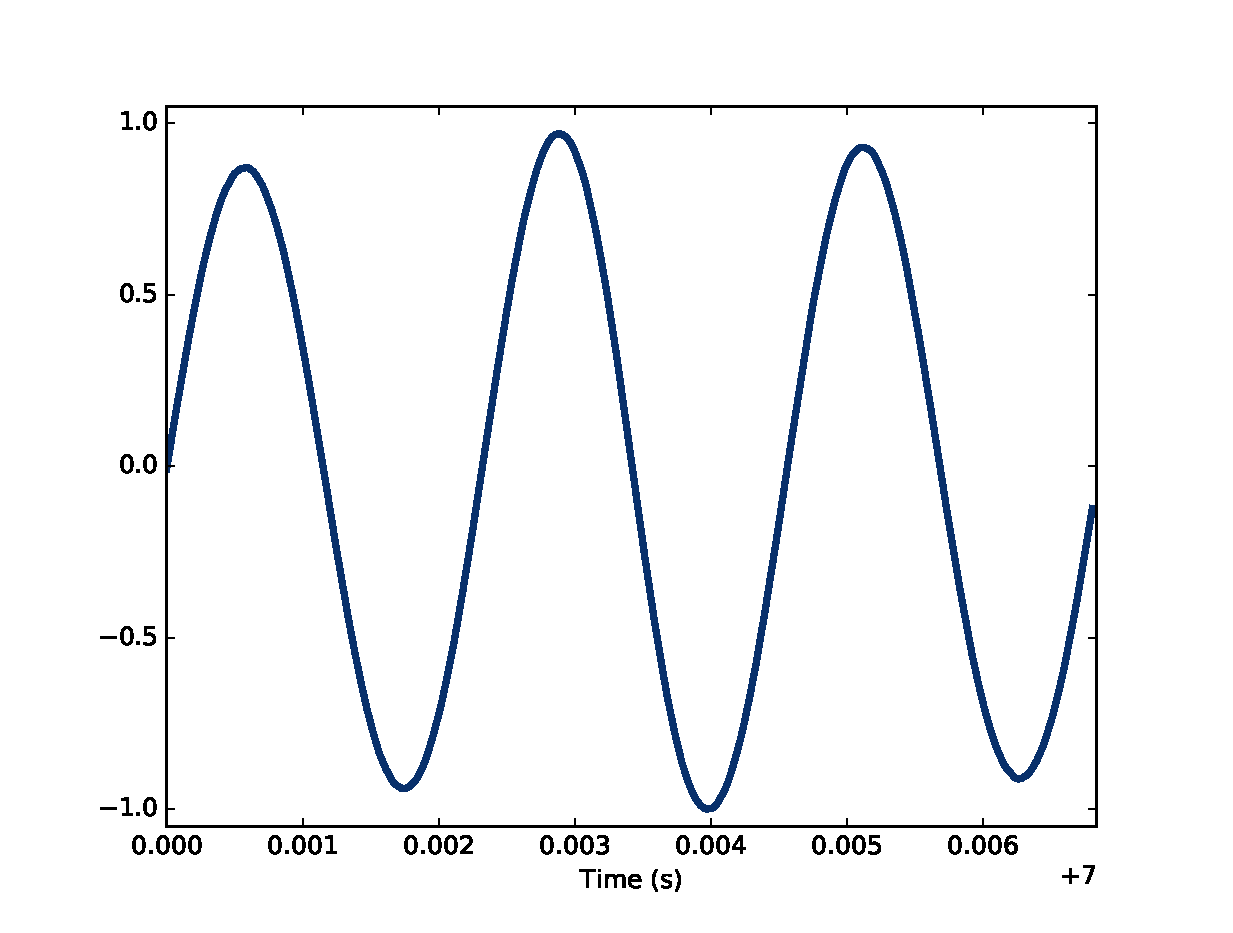
\includegraphics[height=2.5in]{figs/sounds1.eps}}
\caption{Segment from a recording of a bell.}
\label{fig.sounds1}
\end{figure}

We'll start with {\bf periodic signals}, which are signals that
repeat themselves after some period of time.  For example, if you
strike a bell, it vibrates and generates sound.  If you record
that sound and plot the transduced signal, it looks like
Figure~\ref{fig.sounds1}.

This signal resembles a {\bf sinusoid}, which means it has the same
shape as the trigonometric sine function.

You can see that this signal is periodic.  I chose the duration
to show three full periods, also known as {\bf cycles}.
The duration of each cycle is about 2.3 ms.

The {\bf frequency} of a signal is the number of cycles
per second, which is the inverse of the period.
The units of frequency are cycles per second, or {\bf Hertz},
abbreviated ``Hz''.

The frequency of this signal is about 439 Hz, slightly lower than 440
Hz, which is the standard tuning pitch for orchestral music.  The
musical name of this note is A, or more specifically, A4.  If you are
not familiar with ``scientific pitch notation'', the numerical suffix
indicates which octave the note is in.  A4 is the A above middle C.
A5 is one octave higher.  See
\url{http://en.wikipedia.org/wiki/Scientific_pitch_notation}.

\begin{figure}
% sounds.py
\centerline{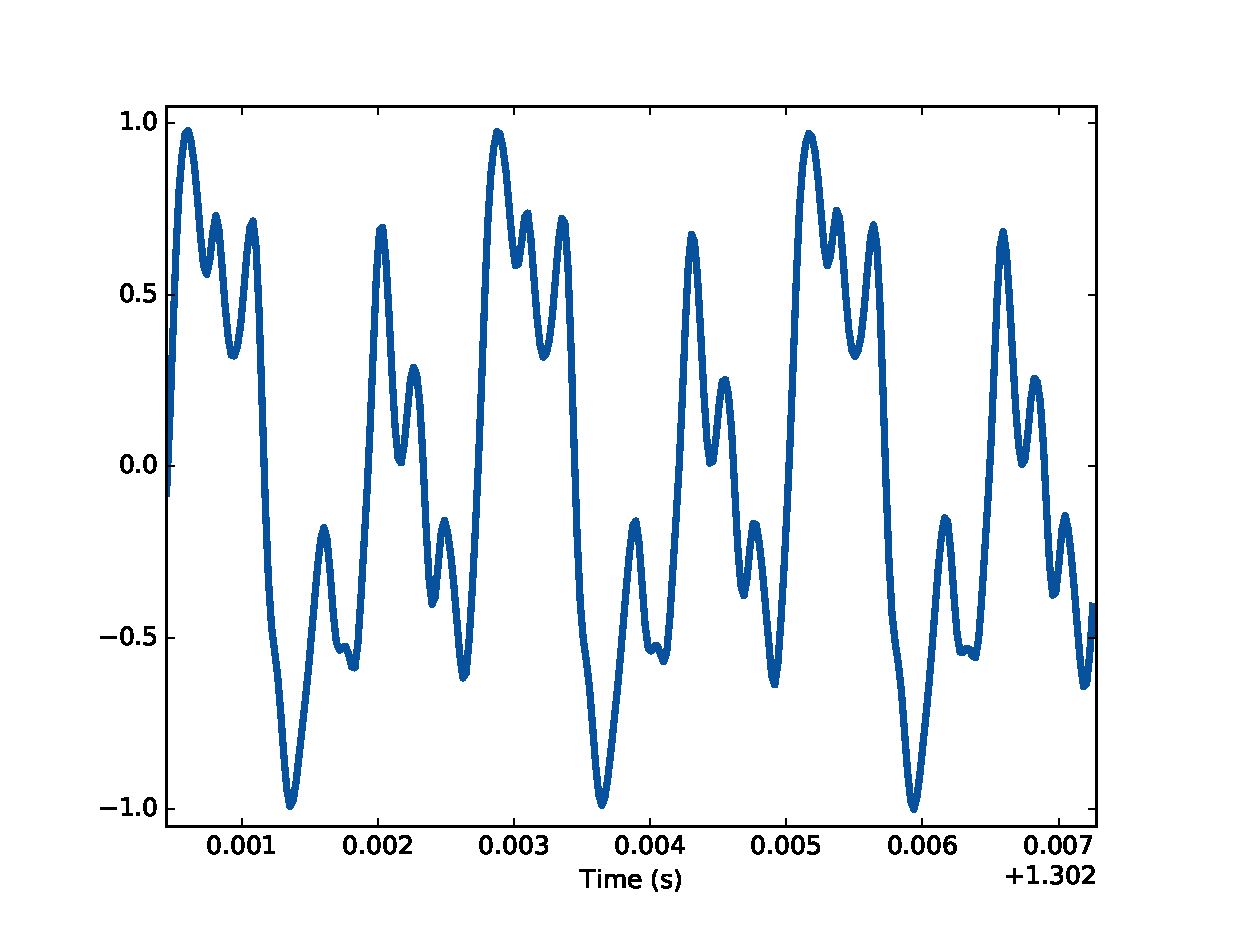
\includegraphics[height=2.5in]{figs/sounds2.eps}}
\caption{Segment from a recording of a violin.}
\label{fig.sounds2}
\end{figure}

A tuning fork generates a sinusoid because the vibration of the tines
is a form of simple harmonic motion.  Most musical instruments
produce periodic signals, but the shape of these signals is not
sinusoidal.  For example, Figure~\ref{fig.sounds2} shows a segment
from a recording of a violin playing
Boccherini's String Quintet No. 5 in E, 3rd
movement.

%\footnote{The recording is from
%  \url{http://www.freesound.org/people/jcveliz/sounds/92002/}.
%I identified the piece using \url{http://www.musipedia.org}.}
% Parson's code: DUUDDUURDR

Again we can see that the signal is periodic, but the shape of the
signal is more complex.  The shape of a periodic signal is called
the {\bf waveform}.  Most musical instruments produce waveforms more
complex than a sinusoid.  The shape of the waveform determines the
musical {\bf timbre}, which is our perception of the quality of the
sound.  People usually perceive complex waveforms as rich, warm and
more interesting than sinusoids.


\section{Spectral decomposition}

\begin{figure}
% sounds.py
\centerline{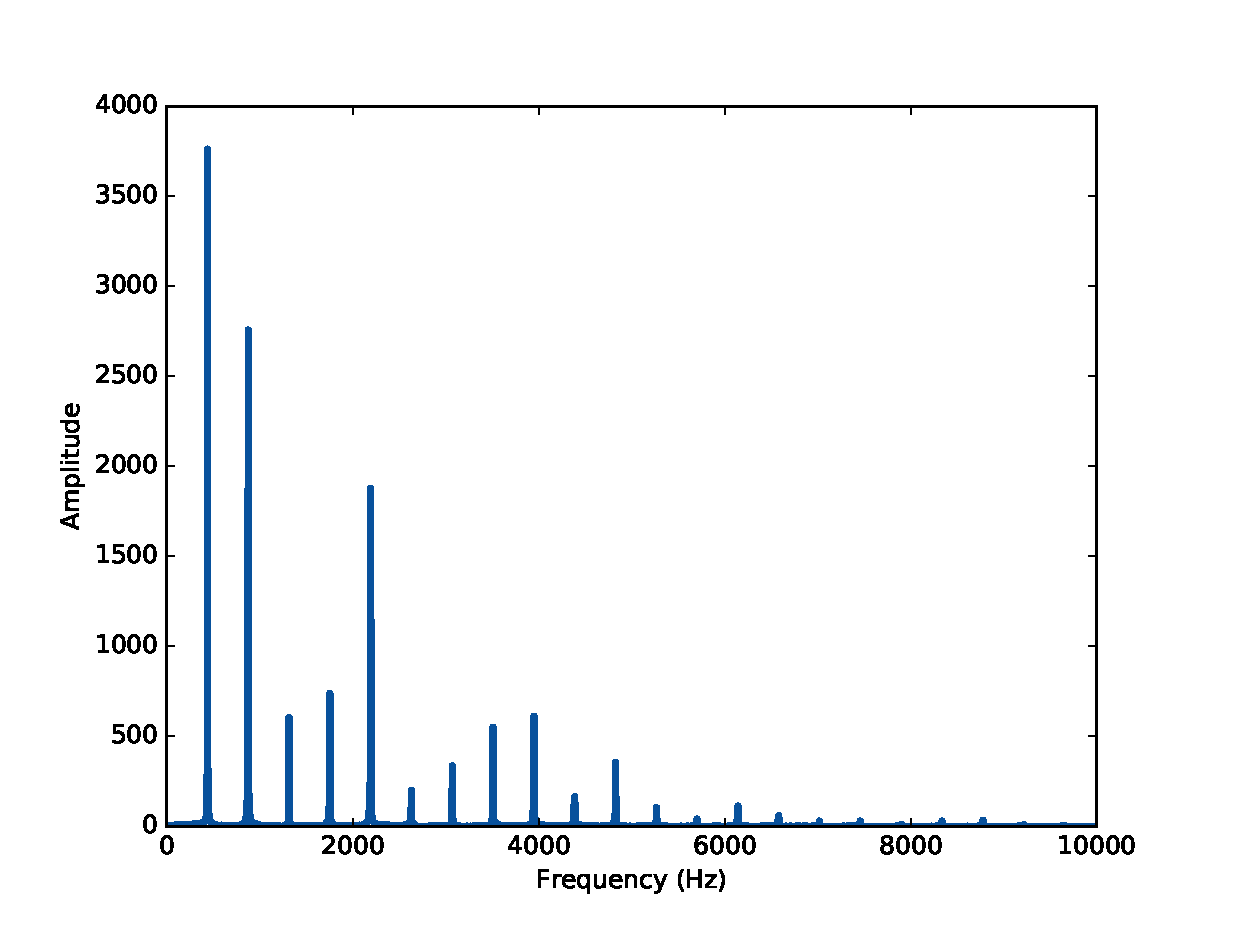
\includegraphics[height=2.5in]{figs/sounds3.eps}}
\caption{Spectrum of a segment from the violin recording.}
\label{fig.sounds3}
\end{figure}

The most important topic in this book is {\bf spectral decomposition},
which is the idea that any signal can be expressed as the sum of
sinusoids with different frequencies.

The most important mathematical idea in this book is the {\bf discrete
  Fourier transform}, or {\bf DFT}, which takes a signal and produces
its {\bf spectrum}.  The spectrum is the set of sinusoids that add up to
produce the signal.

And the most important algorithm in this book is the {\bf Fast
Fourier transform}, or {\bf FFT}, which is an efficient way to
compute the DFT.

For example, Figure~\ref{fig.sounds3} shows the spectrum of the violin
recording in Figure~\ref{fig.sounds2}.  The x-axis is the range of
frequencies that make up the signal.  The y-axis shows the strength
or {\bf amplitude} of each frequency component.

The lowest frequency component is called the {\bf fundamental
  frequency}.  The fundamental frequency of this signal is near 440 Hz
(actually a little lower, or ``flat'').

In this signal the fundamental frequency has the largest amplitude,
so it is also the {\bf dominant frequency}.
Normally the perceived pitch of a sound is determined by the
fundamental frequency, even if it is not dominant. 

The other spikes in the spectrum are at frequencies 880, 1320, 1760, and
2200, which are integer multiples of the fundamental.
These components are called {\bf harmonics} because they are
musically harmonious with the fundamental:

\begin{itemize}

\item 880 is the frequency of A5, one octave higher than the fundamental.  

\item 1320 is approximately E6, which is a major fifth above A5.
  If you are not familiar with musical intervals like "major fifth'', see
  \url{https://en.wikipedia.org/wiki/Interval_(music)}.

\item 1760 is A6, two octaves above the fundamental. 

\item 2200 is approximately C$\sharp$7, which is a major third
above A6.

\end{itemize}

These harmonics make up the notes of an A major
chord, although not all in the same octave.  Some of them are only
approximate because the notes that make up Western music have been
adjusted for {\bf equal temperament} (see
 \url{http://en.wikipedia.org/wiki/Equal_temperament}).

Given the harmonics and their amplitudes, you can reconstruct the
signal by adding up sinusoids.  
Next we'll see how.


\section{Signals}

I wrote a Python module called {\tt thinkdsp.py} that contains classes
and functions for working with signals and spectrums\footnote{The
plural of ``spectrum'' is often written ``spectra'', but I prefer
to use standard English plurals.  If you are familiar with ``spectra'',
I hope my choice doesn't sound too strange.}.  You
will find it in the repository for this book (see Section~\ref{code}).

To represent signals, {\tt thinkdsp} provides a class called
{\tt Signal}, which is the parent class for several signal types,
including {\tt Sinusoid}, which represents both sine and cosine
signals.

{\tt thinkdsp} provides functions to create sine and cosine signals:

\begin{verbatim}
    cos_sig = thinkdsp.CosSignal(freq=440, amp=1.0, offset=0)
    sin_sig = thinkdsp.SinSignal(freq=880, amp=0.5, offset=0)
\end{verbatim}

{\tt freq} is frequency in Hz.  {\tt amp} is amplitude in unspecified
units where 1.0 is defined as the largest amplitude we can record or
play back.

{\tt offset} is a {\bf phase offset} in radians.  Phase offset
determines where in the period the signal starts.  For example, a
sine signal with {\tt offset=0} starts at $\sin 0$, which is 0.
With {\tt offset=pi/2} it starts at $\sin \pi/2$, which is 1.  A cosine
signal with {\tt offset=0} also starts at 0.  In fact, a cosine signal
with {\tt offset=0} is identical to a sine signal with {\tt
  offset=pi/2}.

Signals have an \verb"__add__" method, so you can use the {\tt +}
operator to add them:

\begin{verbatim}
    mix = sin_sig + cos_sig
\end{verbatim}

The result is a {\tt SumSignal}, which represents the sum of two
or more signals.

A Signal is basically a Python representation of a mathematical
function.  Most signals are defined for all values of {\tt t},
from negative infinity to infinity.

You can't do much with a Signal until you evaluate it.  In this
context, ``evaluate'' means taking a sequence of points in time, {\tt
  ts}, and computing the corresponding values of the signal, {\tt ys}.
I represent {\tt ts} and {\tt ys} using NumPy arrays and excapsulate
them in an object called a Wave.

A Wave represents a signal evaluated at a sequence of points in
time.  Each point in time is called a {\bf frame} (a term borrowed
from movies and video).  The measurement itself is called a
{\bf sample}, although ``frame'' and ``sample'' are sometimes
used interchangeably.

{\tt Signal} provides \verb"make_wave", which returns a new
Wave object:

\begin{verbatim}
    wave = mix.make_wave(duration=0.5, start=0, framerate=11025)
\end{verbatim}

{\tt duration} is the length of the Wave in seconds.  {\tt start} is
the start time, also in seconds.  {\tt framerate} is the (integer)
number of frames per second, which is also the number of samples
per second.

11,025 frames per second is one of several framerates commonly used in
audio file formats, including Waveform Audio File (WAV) and mp3. 

This example evaluates the signal from {\tt t=0} to {\tt t=0.5} at
5,513 equally-spaced frames (because 5,513 is half of 11,025).
The time between frames, or {\bf timestep}, is {\tt 1/11025} seconds, or
91 $\mu$s.

{\tt Wave} provides a {\tt plot} method that uses {\tt pyplot}.
You can plot the wave like this:

\begin{verbatim}
    wave.plot()
    pyplot.show()
\end{verbatim}

{\tt pyplot} is part of {\tt matplotlib}; it is included in many
Python distributions, or you might have to install it.

\begin{figure}
% sounds4.py
\centerline{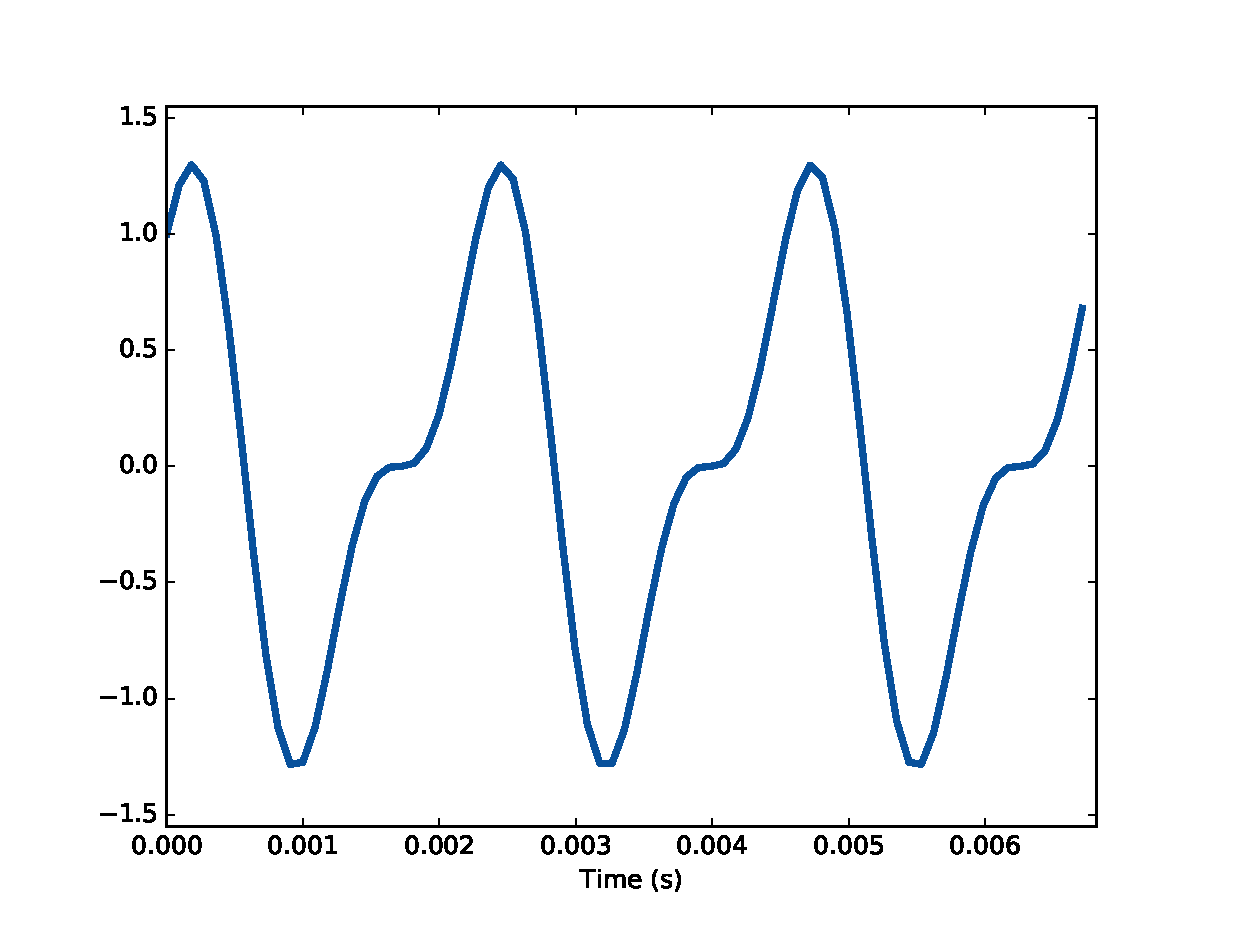
\includegraphics[height=2.5in]{figs/sounds4.eps}}
\caption{Segment from a mixture of two sinusoid signals.}
\label{fig.sounds4}
\end{figure}

At {\tt freq=440} there are 220 periods in 0.5 seconds, so this plot
would look like a solid block of color.  To zoom in on a small number
of periods, we can use {\tt segment}, which copies a segment of a Wave
and returns a new wave:

\begin{verbatim}
    period = mix.period
    segment = wave.segment(start=0, duration=period*3)
\end{verbatim}

{\tt period} is a property of a Signal; it returns the period in seconds.

{\tt start} and {\tt duration} are in seconds.  This example copies
the first three periods from {\tt mix}.  The result is a Wave object.

If we plot {\tt segment}, it looks like Figure~\ref{fig.sounds4}.
This signal contains two frequency components, so it is more
complicated than the signal from the tuning fork, but less complicated
than the violin.


\section{Reading and writing Waves}

{\tt thinkdsp} provides \verb"read_wave", which reads a WAV
file and returns a Wave:

\begin{verbatim}
    violin_wave = thinkdsp.read_wave('input.wav')
\end{verbatim}

And {\tt Wave} provides {\tt write}, which writes a WAV file:

\begin{verbatim}
    wave.write(filename='output.wav')
\end{verbatim}

You can listen to the Wave with any media player that plays WAV
files.  On UNIX systems, I use {\tt aplay}, which is simple, robust,
and included in many Linux distributions.

{\tt thinkdsp} also provides \verb"play_wave", which runs
the media player as a subprocess:

\begin{verbatim}
    thinkdsp.play_wave(filename='output.wav', player='aplay')
\end{verbatim}

It uses {\tt aplay} by default, but you can provide the
name of another player.


\section{Spectrums}
\label{spectrums}

{\tt Wave} provides \verb"make_spectrum", which returns a
{\tt Spectrum}:

\begin{verbatim}
    spectrum = wave.make_spectrum()
\end{verbatim}

And {\tt Spectrum} provides {\tt plot}:

\begin{verbatim}
    spectrum.plot()
    thinkplot.show()
\end{verbatim}

{\tt thinkplot} is a module I wrote to provide wrappers around some of
the functions in {\tt pyplot}.  It is included in the
Git repository for this book (see Section~\ref{code}).

{\tt Spectrum} provides three methods that modify the spectrum:

\begin{itemize}

\item \verb"low_pass" applies a low-pass filter, which means that
  components above a given cutoff frequency are attenuated (that is,
  reduced in magnitude) by a factor.

\item \verb"high_pass" applies a high-pass filter, which means that
  it attenuates components below the cutoff.

\item \verb"band_stop" attenuates components in the band of
frequencies between two cutoffs.

\end{itemize}

This example attenuates all frequencies above 600 by 99\%:

\begin{verbatim}
   spectrum.low_pass(cutoff=600, factor=0.01)
\end{verbatim}

A low pass filter removes bright, high-frequency sounds, so
the result sounds muffled and darker.  To hear what it sounds
like, you can convert the Spectrum back to a Wave, and then play it.

\begin{verbatim}
    wave = spectrum.make_wave()
    wave.play('temp.wav')
\end{verbatim}

The {\tt play} method writes the wave to a file and then plays it.
If you use IPython notebooks, you can use \verb"make_audio", which
makes an Audio widget that plays the sound.


\section{Wave objects}

\begin{figure}
% http://yuml.me/edit/5294b377
% pdftops -eps diagram1.pdf
\centerline{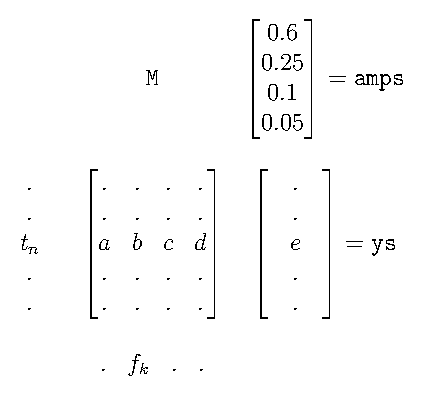
\includegraphics[width=3.5in]{figs/diagram1.eps}}
\caption{Relationships among the classes in {\tt thinkdsp}.}
\label{fig.diagram1}
\end{figure}

There is nothing very complicated in {\tt thinkdsp.py}.  Most
of the functions it provides are thin wrappers around functions
from NumPy and SciPy.

The primary classes in {\tt thinkdsp} are Signal, Wave, and Spectrum.
Given a Signal, you can make a Wave.  Given a Wave, you can
make a Spectrum, and vice versa.  These relationships are shown
in Figure~\ref{fig.diagram1}.

A Wave object contains three attributes: {\tt ys} is a NumPy array
that contains the values in the signal; {\tt ts} is an array of the
times where the signal was evaluated or sampled; and {\tt
  framerate} is the number of samples per unit of time.  The
unit of time is usually seconds, but it doesn't have to be.  In
one of my examples, it's days.

Wave also provides three read-only properties: {\tt start},
{\tt end}, and {\tt duration}.  If you modify {\tt ts}, these
properties change accordingly.

To modify a wave, you can access the {\tt ts} and {\tt ys} directly.
For example:

\begin{verbatim}
wave.ys *= 2
wave.ts += 1
\end{verbatim} 

The first line scales the wave by a factor of 2, making
it louder.  The second line shifts the wave in time, making it
start 1 second later.

But Wave provides methods that perform many common operations.
For example, the same two transformations could be written:

\begin{verbatim}
wave.scale(2)
wave.shift(1)
\end{verbatim} 

You can read the documentation of these methods and others at
\url{http://think-dsp.com/thinkdsp.html}.


\section{Signal objects}
\label{sigobs}

Signal is a parent class that provides functions common to all
kinds of signals, like \verb"make_wave".  Child classes inherit
these methods and provide {\tt evaluate}, which evaluates the
signal at a given sequence of times.

For example, Sinusoid is a child class of Signal, with this
definition:

\begin{verbatim}
class Sinusoid(Signal):
    
    def __init__(self, freq=440, amp=1.0, offset=0, func=np.sin):
        Signal.__init__(self)
        self.freq = freq
        self.amp = amp
        self.offset = offset
        self.func = func
\end{verbatim}

The parameters of \verb"__init__" are:

\begin{itemize}

\item {\tt freq}: frequency in cycles per second, or Hz.

\item {\tt amp}: amplitude.  The units of amplitude are arbitrary,
usually chosen so 1.0 corresponds to the maximum input from a
microphone or maximum output to a speaker.

\item {\tt offset}: indicates where in its period the signal starts;
{\tt offset} is in units of radians, for reasons I explain below.

\item {\tt func}: a Python function used
to evaluate the signal at a particular point in time.  It is
usually either {\tt np.sin} or {\tt np.cos}, yielding a sine or
cosine signal.

\end{itemize}

Like many init methods, this one just tucks the parameters away for
future use.

Signal provides \verb"make_wave", which looks like
this:

\begin{verbatim}
    def make_wave(self, duration=1, start=0, framerate=11025):
        n = round(duration * framerate)
        ts = start + np.arange(n) / framerate
        ys = self.evaluate(ts)
        return Wave(ys, ts, framerate=framerate)
\end{verbatim}

{\tt start} and {\tt duration} are the start time and duration
in seconds.  {\tt framerate} is the number of frames (samples)
per second.

{\tt n} is the number of samples, and {\tt ts} is a NumPy array
of sample times.

To compute the {\tt ys}, \verb"make_wave" invokes {\tt evaluate}, 
is provided by {\tt Sinusoid}:

\begin{verbatim}
    def evaluate(self, ts):
        phases = PI2 * self.freq * ts + self.offset
        ys = self.amp * self.func(phases)
        return ys
\end{verbatim}

Let's unwind this function one step at time:

\begin{enumerate}

\item {\tt self.freq} is frequency in cycles per second, and each
  element of {\tt ts} is a time in seconds, so their product is the
  number of cycles since the start time.

\item {\tt PI2} is a constant that stores $2 \pi$.  Multiplying by
  {\tt PI2} converts from cycles to {\bf phase}.  You can think of
  phase as ``cycles since the start time'' expressed in radians.  Each
  cycle is $2 \pi$ radians.

\item {\tt self.offset} is the phase when $t=0$.
  It has the effect of shifting the signal left or right in time.

\item If {\tt self.func} is {\tt np.sin} or {\tt np.cos}, the result is a
  value between $-1$ and $+1$.

\item Multiplying by {\tt self.amp} yields a signal that ranges from
  {\tt -self.amp} to {\tt +self.amp}.

\end{enumerate}

In math notation, {\tt evaluate} is written like this:
%
\[ y = A \cos (2 \pi f t + \phi_0) \]
%
where $A$ is amplitude, $f$ is frequency, $t$ is time, and $\phi_0$
is the phase offset.  It may seem like I wrote a lot of code
to evaluate one simple expression, but as we'll see, this code
provides a framework for dealing with all kinds of signals, not
just sinusoids.


\section{Exercises}

Before you begin these exercises, you should download the code
for this book, following the instructions in Section~\ref{code}.

Solutions to these exercises are in {\tt chap01soln.ipynb}.

\begin{exercise}
If you have IPython, load {\tt chap01.ipynb}, read through it, and run
the examples.  You can also view this notebook at
\url{http://tinyurl.com/thinkdsp01}.
\end{exercise}


\begin{exercise}
Go to \url{http://freesound.org} and download a sound sample that
includes music, speech, or other sounds that have a well-defined pitch.
Select a roughly half-second segment where the pitch is
constant.  Compute and plot the spectrum of the segment you selected.
What connection can you make between the timbre of the sound and the
harmonic structure you see in the spectrum?

Use \verb"high_pass", \verb"low_pass", and \verb"band_stop" to
filter out some of the harmonics.  Then convert the spectrum back
to a wave and listen to it.  How does the sound relate to the
changes you made in the spectrum?
\end{exercise}


\begin{exercise}
Synthesize a compound signal by creating SinSignal and CosSignal
objects and adding them up.  Evaluate the signal to get a Wave,
and listen to it.  Compute its Spectrum and plot it.
What happens if you add frequency
components that are not multiples of the fundamental?
\end{exercise}


\begin{exercise}
Write a function called {\tt stretch} that takes a Wave and a stretch
factor and speeds up or slows down the wave by modifying {\tt ts} and
{\tt framerate}.  Hint: it should only take two lines of code.
\end{exercise}


\chapter{Harmonics}
\label{harmonics}

In this chapter I present several new waveforms; we will look and
their spectrums to understand their {\bf harmonic structure}, which is
the set of sinusoids they are made up of.

I'll also introduce one of the most important phenomena in digital
signal processing: aliasing.  And I'll explain a little more about how
the Spectrum class works.

The code for this chapter is in {\tt chap02.ipynb}, which is in the
repository for this book (see Section~\ref{code}).
You can also view it at \url{http://tinyurl.com/thinkdsp02}.


\section{Triangle waves}
\label{triangle}

A sinusoid contains only one frequency component, so its spectrum
has only one peak.  More complicated waveforms, like the
violin recording, yield DFTs with many peaks.  In this section we
investigate the relationship between waveforms and their spectrums.

\begin{figure}
% aliasing.py
\centerline{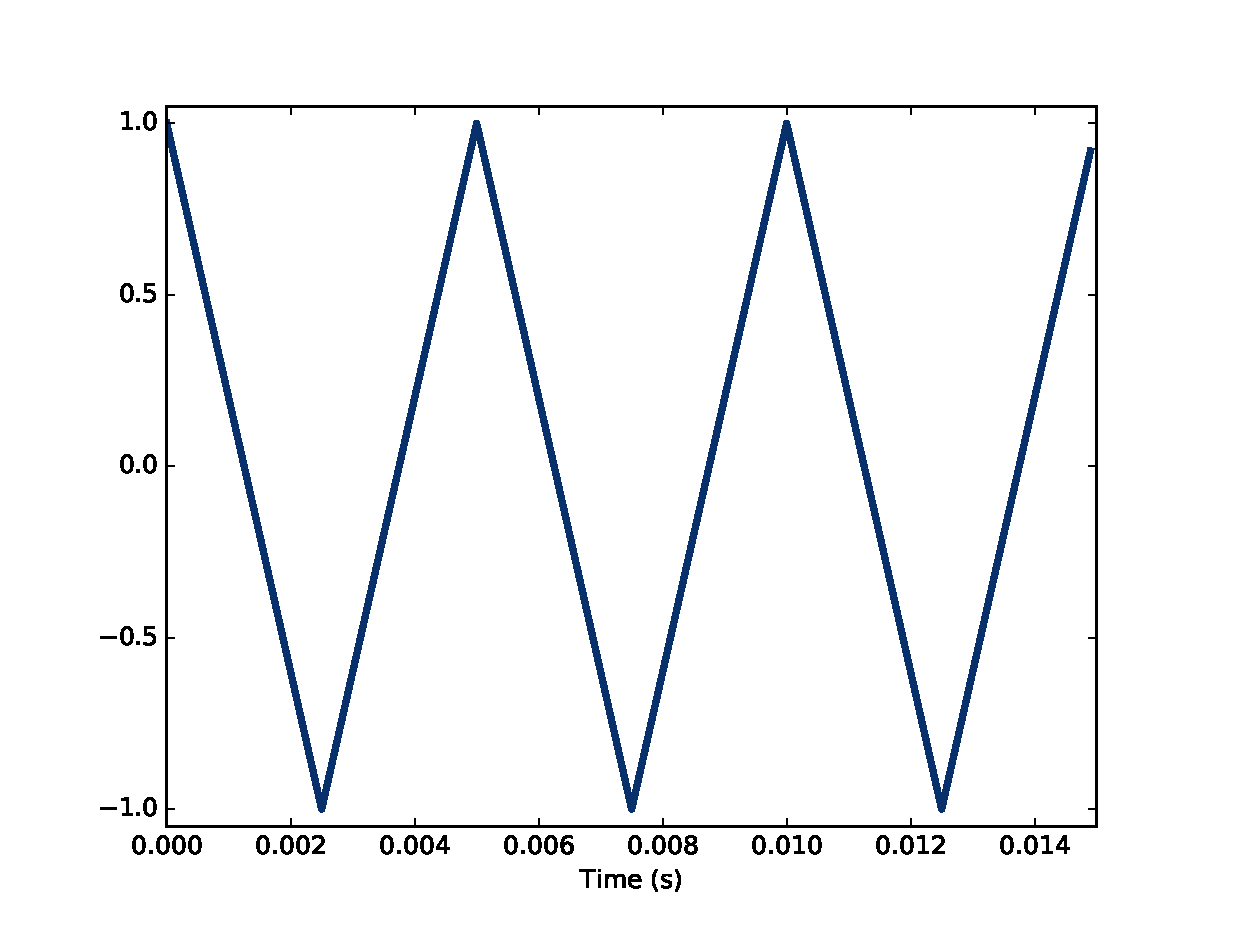
\includegraphics[height=2.5in]{figs/triangle-200-1.eps}}
\caption{Segment of a triangle signal at 200 Hz.}
\label{fig.triangle.200.1}
\end{figure}

I'll start with a triangle waveform, which is like a straight-line
version of a sinusoid.  Figure~\ref{fig.triangle.200.1} shows a
triangle waveform with frequency 200 Hz.

To generate a triangle wave, you can use {\tt thinkdsp.TriangleSignal}:

\begin{verbatim}
class TriangleSignal(Sinusoid):
    
    def evaluate(self, ts):
        cycles = self.freq * ts + self.offset / PI2
        frac, _ = np.modf(cycles)
        ys = np.abs(frac - 0.5)
        ys = normalize(unbias(ys), self.amp)
        return ys
\end{verbatim}

{\tt TriangleSignal} inherits \verb"__init__" from {\tt Sinusoid},
so it takes the same arguments: {\tt freq}, {\tt amp}, and {\tt offset}.

The only difference is {\tt evaluate}.  As we saw before,
{\tt ts} is the sequence of sample times where we want to
evaluate the signal.

There are many ways to generate a triangle wave.  The details
are not important, but here's how {\tt evaluate} works:

\begin{enumerate}

\item {\tt cycles} is the number of cycles since the start time.
{\tt np.modf} splits the number of cycles into the fraction
part, stored in {\tt frac}, and the integer part, which is ignored
\footnote{Using an underscore as a variable name is a convention that
means, ``I don't intend to use this value.''}.

\item {\tt frac} is a sequence that ramps from 0 to 1 with the given
  frequency.  Subtracting 0.5 yields values between -0.5 and 0.5.
  Taking the absolute value yields a waveform that zig-zags between
  0.5 and 0.

\item {\tt unbias} shifts the waveform down so it is centered at 0; then
{\tt normalize} scales it to the given amplitude, {\tt amp}.

\end{enumerate}

Here's the code that generates Figure~\ref{fig.triangle.200.1}:

\begin{verbatim}
signal = thinkdsp.TriangleSignal(200)
signal.plot()
\end{verbatim}

\begin{figure}
% aliasing.py
\centerline{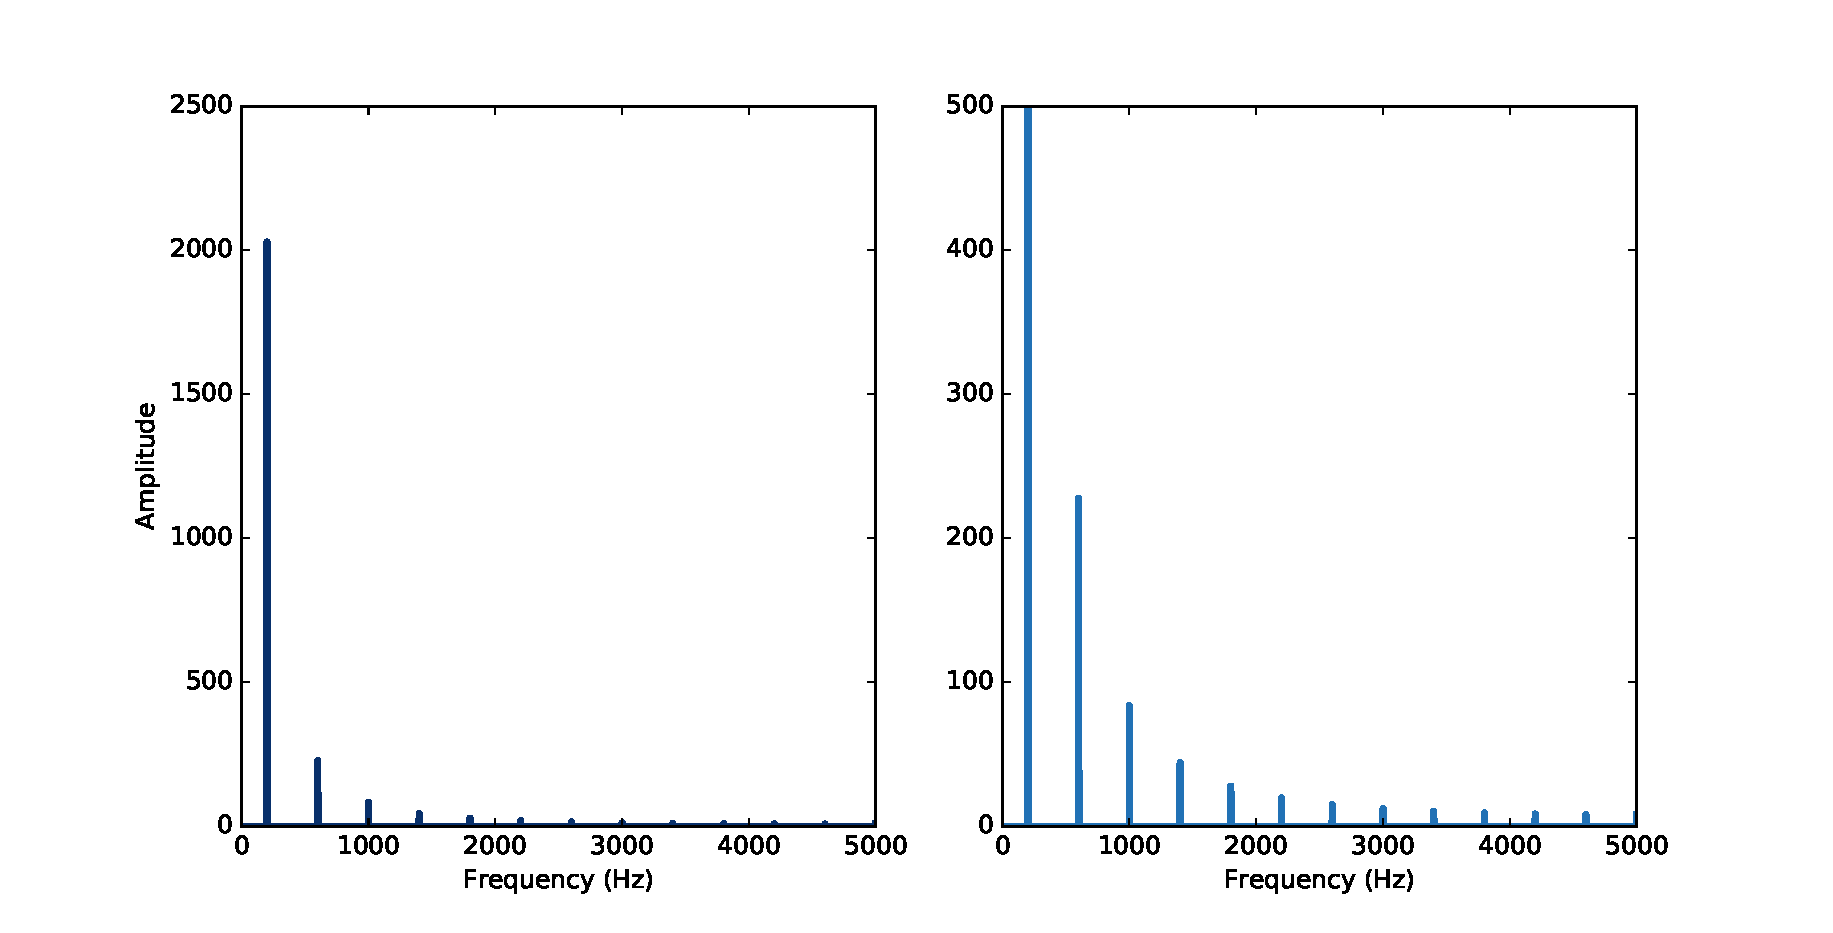
\includegraphics[height=2.5in]{figs/triangle-200-2.eps}}
\caption{Spectrum of a triangle signal at 200 Hz.}
\label{fig.triangle.200.2}
\end{figure}

Next we can use the Signal to make a Wave, and use the Wave to
make a Spectrum:

\begin{verbatim}
wave = signal.make_wave(duration=0.5, framerate=10000)
spectrum = wave.make_spectrum()
spectrum.plot()
\end{verbatim}

Figure~\ref{fig.triangle.200.2} shows the result.  As expected, the
highest peak is at the fundamental frequency, 200 Hz, and there
are additional peaks at harmonic frequencies, which are integer
multiples of 200.

But one surprise is that there are no peaks at the even multiples:
400, 800, etc.  The harmonics of a triangle wave are all
odd multiples of the fundamental frequency, in this example
600, 1000, 1400, etc.

Another feature of this spectrum is the relationship between the
amplitude and frequency of the harmonics.  Their amplitude drops off
in proportion to frequency squared.  For example the frequency ratio
of the first two harmonics (200 and 600 Hz) is 3, and the amplitude
ratio is approximately 9.  The frequency ratio of the next two
harmonics (600 and 1000 Hz) is 1.7, and the amplitude ratio is
approximately $1.7^2 = 2.9$.  This relationship is called the
{\bf harmonic structure}.


\section{Square waves}
\label{square}

\begin{figure}
% aliasing.py
\centerline{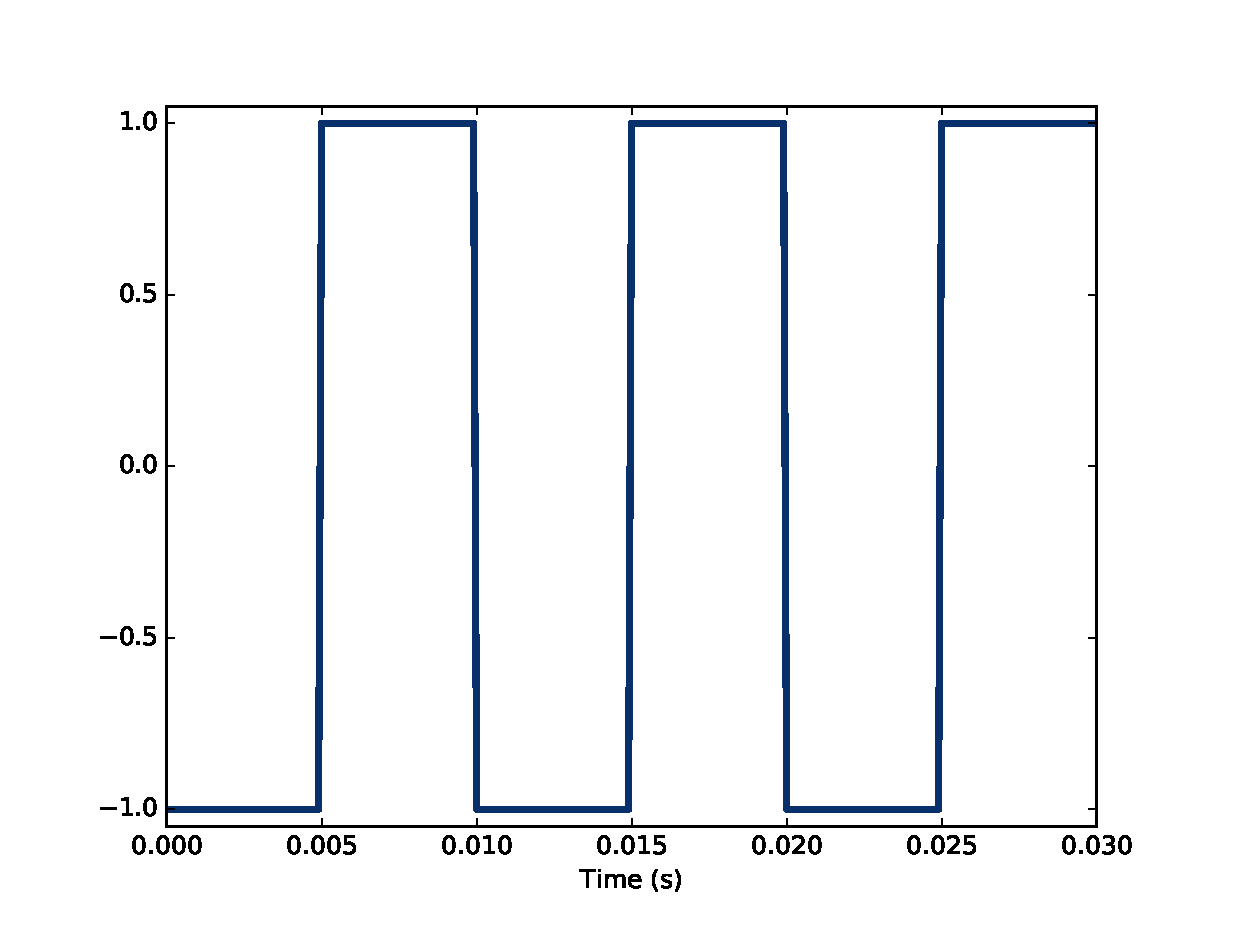
\includegraphics[height=2.5in]{figs/square-100-1.eps}}
\caption{Segment of a square signal at 100 Hz.}
\label{fig.square.100.1}
\end{figure}

{\tt thinkdsp} also provides {\tt SquareSignal}, which represents
a square signal.  Here's the class definition:

\begin{verbatim}
class SquareSignal(Sinusoid):
    
    def evaluate(self, ts):
        cycles = self.freq * ts + self.offset / PI2
        frac, _ = np.modf(cycles)
        ys = self.amp * np.sign(unbias(frac))
        return ys
\end{verbatim}

Like {\tt TriangleSignal}, {\tt SquareSignal} inherits 
\verb"__init__" from {\tt Sinusoid}, so it takes the same
parameters.

And the {\tt evaluate} method is similar.  Again, {\tt cycles} is
the number of cycles since the start time, and {\tt frac} is the
fractional part, which ramps from 0 to 1 each period.

{\tt unbias} shifts {\tt frac} so it ramps from -0.5 to 0.5,
then {\tt np.sign} maps the negative values to -1 and the
positive values to 1.  Multiplying by {\tt amp} yields a square
wave that jumps between {\tt -amp} and {\tt amp}.

\begin{figure}
% aliasing.py
\centerline{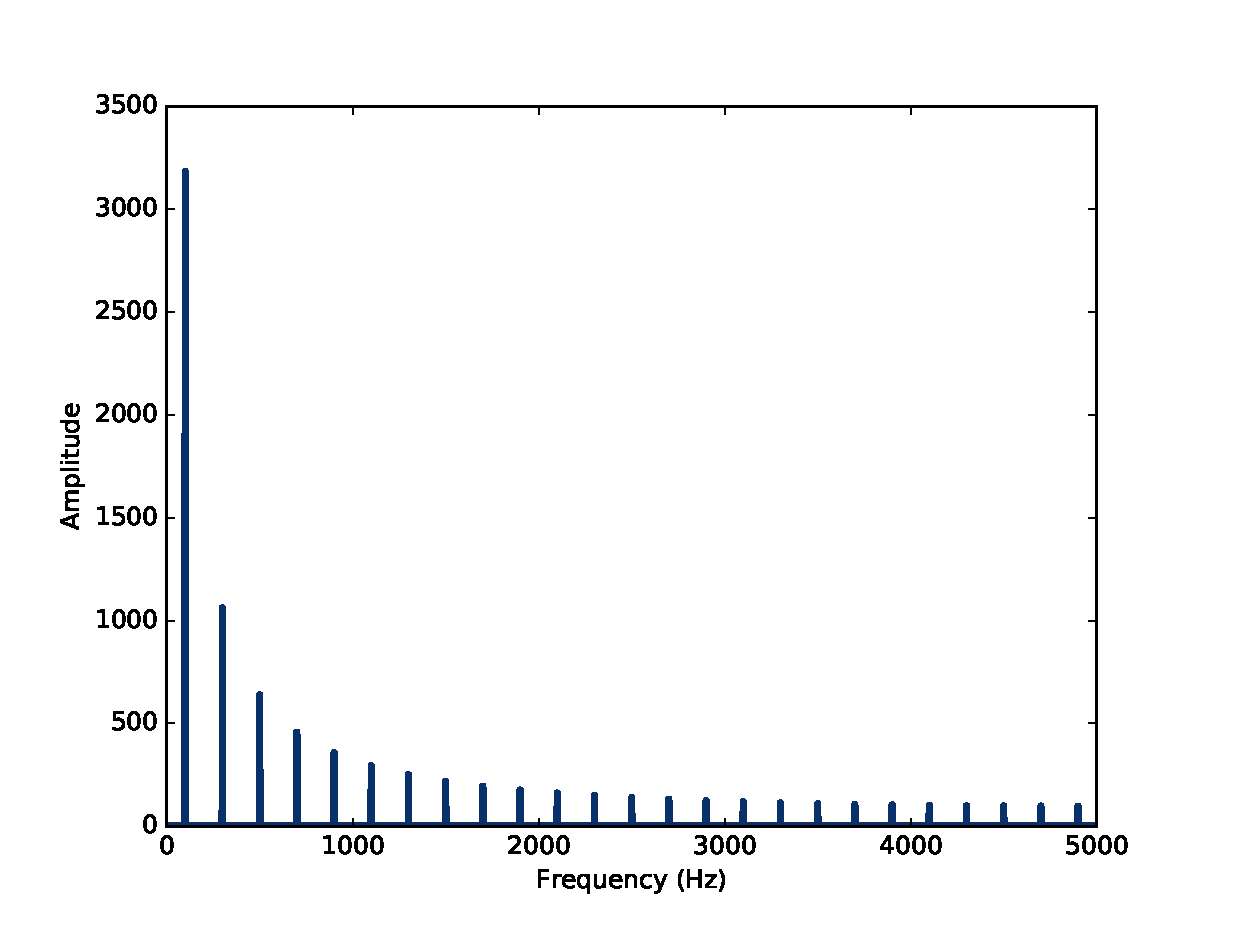
\includegraphics[height=2.5in]{figs/square-100-2.eps}}
\caption{Spectrum of a square signal at 100 Hz.}
\label{fig.square.100.2}
\end{figure}

Figure~\ref{fig.square.100.1} shows three periods of a square
wave with frequency 100 Hz,
and Figure~\ref{fig.square.100.2} shows its spectrum.

Like a triangle wave, the square wave contains only odd harmonics,
which is why there are peaks at 300, 500, and 700 Hz, etc.
But the amplitude of the harmonics drops off more slowly.
Specifically, amplitude drops in proportion to frequency (not frequency
squared).

The exercises at the end of this chapter give you a chance to
explore other waveforms and other harmonic structures.


\section{Aliasing}
\label{aliasing}

\begin{figure}
% aliasing.py
\centerline{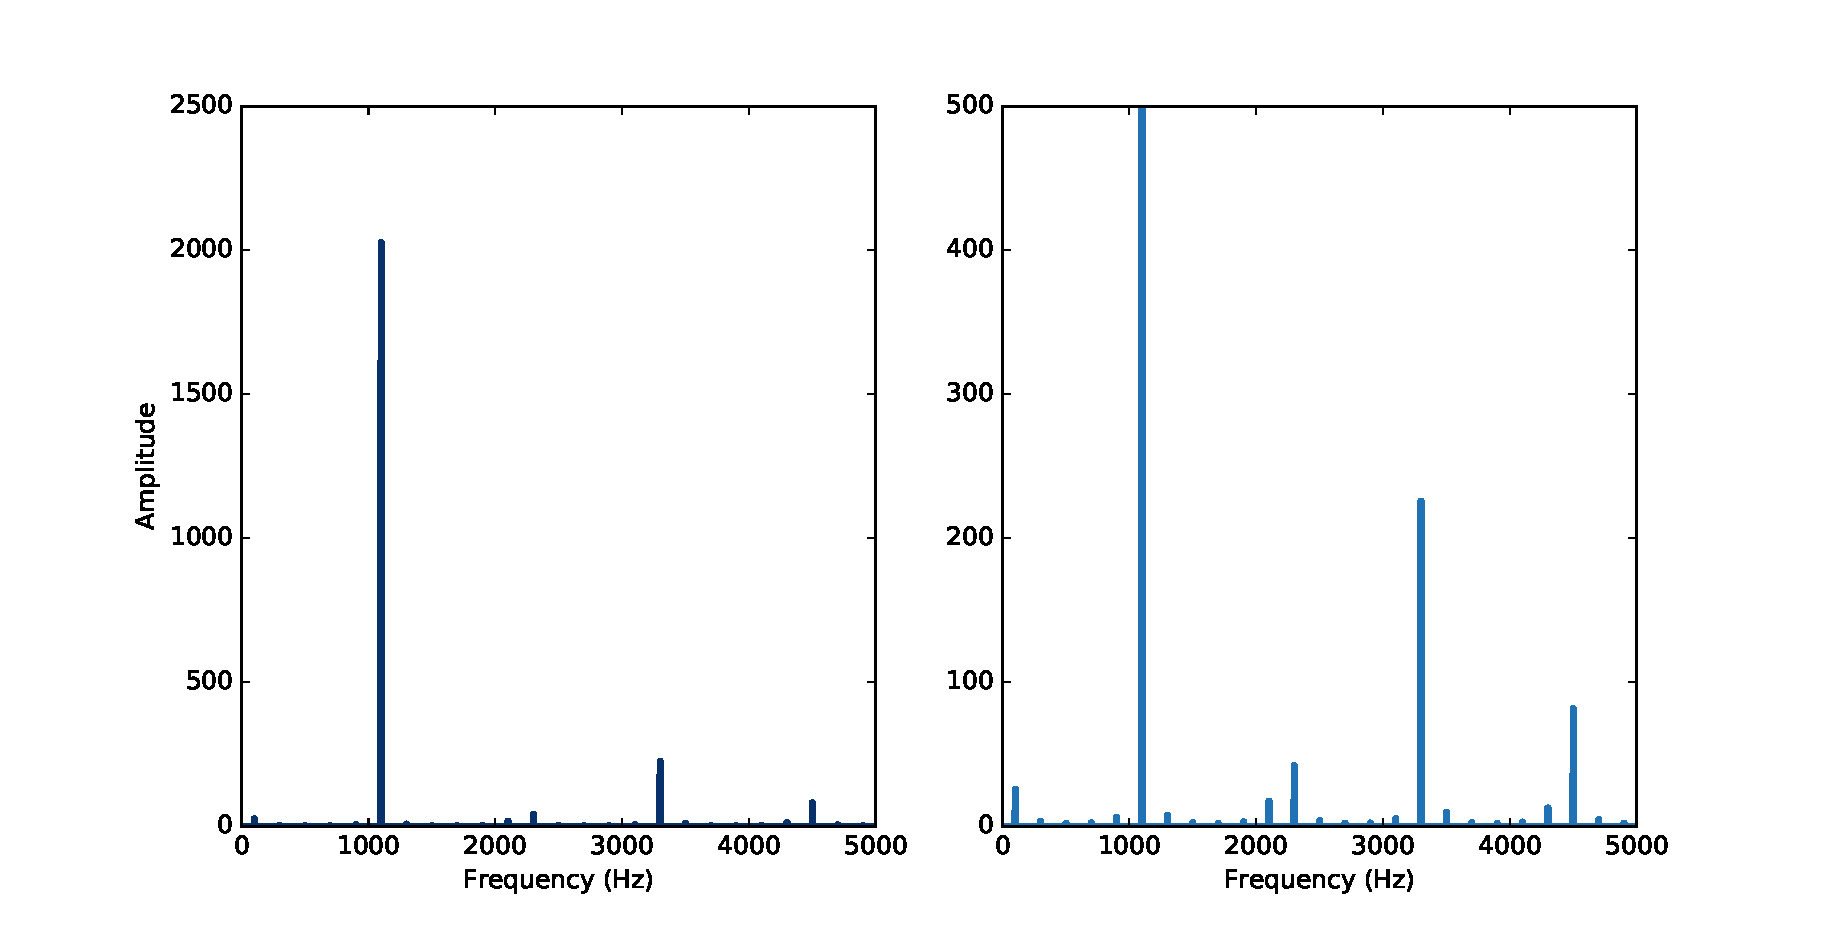
\includegraphics[height=2.5in]{figs/triangle-1100-2.eps}}
\caption{Spectrum of a triangle signal at 1100 Hz sampled at
10,000 frames per second.}
\label{fig.triangle.1100.2}
\end{figure}

I have a confession.  I chose the examples in the previous section
carefully to avoid showing you something confusing.  But now it's
time to get confused.

Figure~\ref{fig.triangle.1100.2} shows the spectrum of a triangle wave
at 1100 Hz, sampled at 10,000 frames per second.  The harmonics
of this wave should be at 3300, 5500, 7700, and 9900 Hz.

In the figure, there are peaks at 1100 and 3300 Hz, as expected, but
the third peak is at 4500, not 5500 Hz.  The
fourth peak is at 2300, not 7700 Hz.  And if you look closely, the
peak that should be at 9900 is actually at 100 Hz.  What's going on?

The problem is that when you evaluate the signal at
discrete points in time, you lose information about what happened
between samples.  For low frequency components, that's not a
problem, because you have lots of samples per period.

But if you sample a signal at 5000 Hz with 10,000 frames per second,
you only have two samples per period.  That turns out to be enough,
just barely, but if the frequency is higher, it's not.

To see why, let's generate cosine signals at 4500 and 5500 Hz,
and sample them at 10,000 frames per second:

\begin{verbatim}
    framerate = 10000

    signal = thinkdsp.CosSignal(4500)
    duration = signal.period*5
    segment = signal.make_wave(duration, framerate=framerate)
    segment.plot()

    signal = thinkdsp.CosSignal(5500)
    segment = signal.make_wave(duration, framerate=framerate)
    segment.plot()
\end{verbatim}

\begin{figure}
% aliasing.py
\centerline{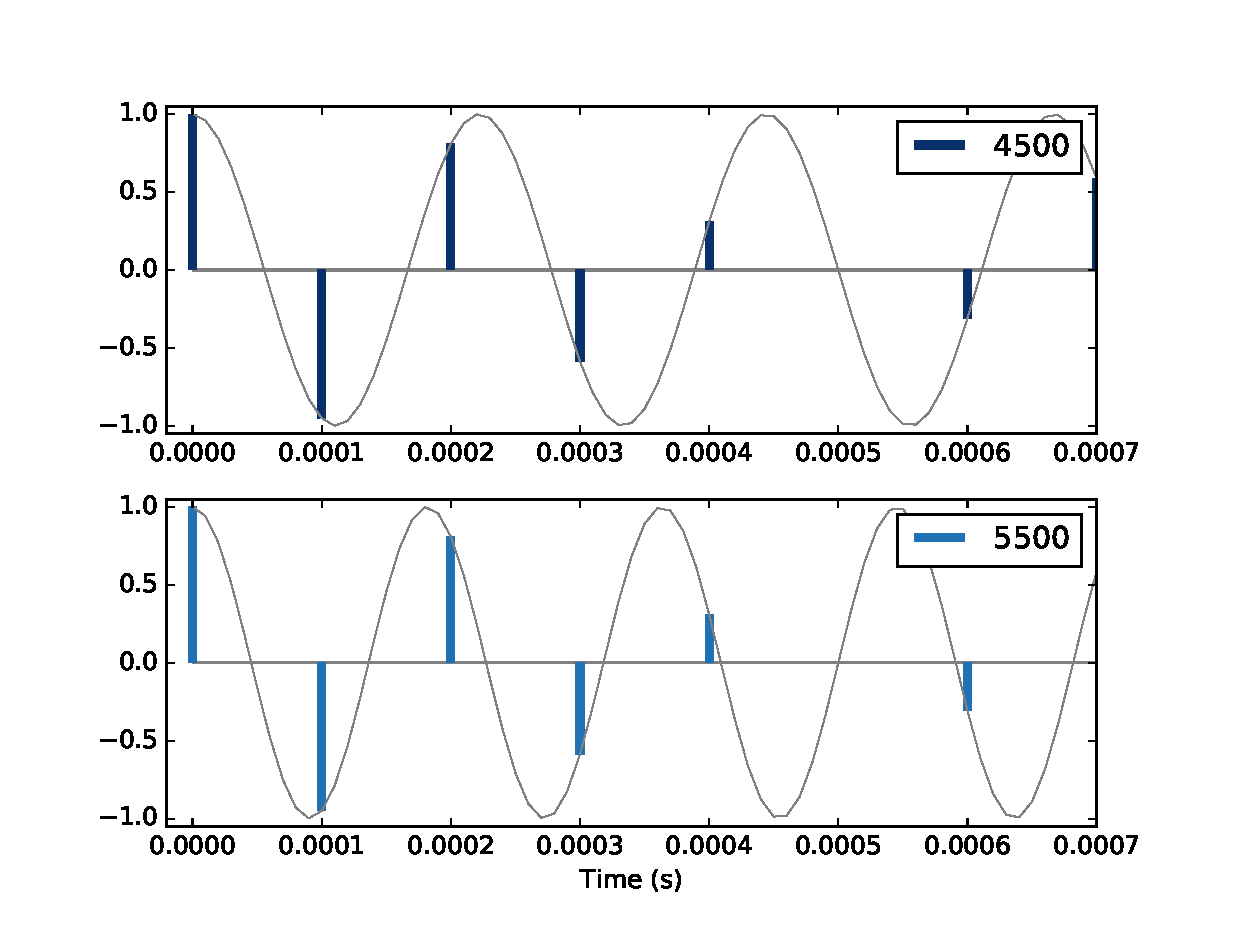
\includegraphics[height=2.5in]{figs/aliasing1.eps}}
\caption{Cosine signals at 4500 and 5500 Hz, sampled at 10,000 frames
per second.  They are identical.}
\label{fig.aliasing1}
\end{figure}

Figure~\ref{fig.aliasing1} shows the result.  I plotted the
samples using vertical lines, to make it easier to compare the
two Waves, and I offset them slightly in time.  The problem
should be clear: the
the two Waves are exactly the same!

When we sample a 5500 Hz signal at 10,000 frames per second, the
result is indistinguishable from a 4500 Hz signal.
For the same reason, a 7700 Hz signal is indistinguishable
from 2300 Hz, and a 9900 Hz is indistinguishable from 100 Hz.

This effect is called {\bf aliasing} because when the high frequency
signal is sampled, it appears to be a low frequency signal.

In this example, the highest frequency we can measure is 5000 Hz,
which is half the sampling rate.  Frequencies above 5000 Hz are folded
back below 5000 Hz, which is why this threshold is sometimes called
the ``folding frequency''.  Is is sometimes also called the {\bf
  Nyquist frequency}.  See
\url{http://en.wikipedia.org/wiki/Nyquist_frequency}.

The folding pattern continues if the aliased frequency goes below
zero.  For example, the 5th harmonic of the 1100 Hz triangle wave is
at 12,100 Hz.  Folded at 5000 Hz, it would appear at -2100 Hz, but it
gets folded again at 0 Hz, back to 2100 Hz.  In fact, you can see a
small peak at 2100 Hz in Figure~\ref{fig.square.100.2}, and the next
one at 4300 Hz.


\section{Computing the spectrum}

We have seen the Wave method \verb"make_spectrum" several times.
Here is the implementation (leaving out some details we'll get
to later):

\begin{verbatim}
from np.fft import rfft, rfftfreq

# class Wave:
    def make_spectrum(self):
        n = len(self.ys)
        d = 1 / self.framerate

        hs = rfft(self.ys)
        fs = rfftfreq(n, d)

        return Spectrum(hs, fs, self.framerate)
\end{verbatim}

The parameter {\tt self} is a Wave object.  {\tt n} is the number
of samples in the wave, and {\tt d} is the inverse of the
frame rate, which is the time between samples.

{\tt np.fft} is the NumPy module that provides functions related
to the {\bf Fast Fourier Transform} (FFT), which is an efficient
algorithm that computes the Discrete Fourier Transform (DFT).

%TODO: add a forward reference to full fft
\verb"make_spectrum" uses {\tt rfft}, which stands for ``real
FFT'', because the Wave contains real values, not complex.  Later
we'll see the full FFT, which can handle complex signals.  The result
of {\tt rfft}, which I call {\tt hs}, is a NumPy array of complex
numbers that represents the amplitude and phase offset of each
frequency component in the wave.

The result of {\tt rfftfreq}, which I call {\tt fs}, is an array that
contains frequencies corresponding to the {\tt hs}. 

To understand the values in {\tt hs}, consider these two ways to think
about complex numbers:

\begin{itemize}

\item A complex number is the sum of a real part and an imaginary
  part, often written $x + iy$, where $i$ is the imaginary unit,
  $\sqrt{-1}$.  You can think of $x$ and $y$ as Cartesian coordinates.

\item A complex number is also the product of a magnitude and a
  complex exponential, $A e^{i \phi}$, where $A$ is the {\bf
    magnitude} and $\phi$ is the {\bf angle} in radians, also called
  the ``argument''.  You can think of $A$ and $\phi$ as polar
  coordinates.

\end{itemize}

Each value in {\tt hs} corresponds to a frequency component: its
magnitude is proportional to the amplitude of the corresponding
component; its angle is the phase offset.

The Spectrum class provides two read-only properties, {\tt amps}
and {\tt angles}, which return NumPy arrays representing the
magnitudes and angles of the {\tt hs}.  When we plot a Spectrum
object, we usually plot {\tt amps} versus {\tt fs}.  Sometimes
it is also useful to plot {\tt angles} versus {\tt fs}.

Although it might be tempting to look at the real and imaginary
parts of {\tt hs}, you will almost never need to.  I encourage
you to think of the DFT as a vector of amplitudes and phase offsets
that happen to be encoded in the form of complex numbers.

To modify a Spectrum, you can access the {\tt hs} directly.
For example:

\begin{verbatim}
spectrum.hs *= 2
spectrum.hs[spectrum.fs > cutoff] = 0
\end{verbatim}

The first line multiples the elements of {\tt hs} by 2, which
doubles the amplitudes of all components.  The second line
sets to 0 only the elements of {\tt hs} where the corresponding
frequency exceeds some cutoff frequency.

But Spectrum also provides methods to perform these operations:

\begin{verbatim}
spectrum.scale(2)
spectrum.low_pass(cutoff)
\end{verbatim}

You can read the documentation of these methods and others at
\url{http://think-dsp.com/thinkdsp.html}.

At this point you should have a better idea of how the Signal, Wave,
and Spectrum classes work, but I have not explained how the Fast
Fourier Transform works.  That will take a few more chapters.


\section{Exercises}

Solutions to these exercises are in {\tt chap02soln.ipynb}.

\begin{exercise}
If you use IPython, load {\tt chap02.ipynb} and try out the examples.
You can also view the notebook at \url{http://tinyurl.com/thinkdsp02}.
\end{exercise}

\begin{exercise}
A sawtooth signal has a waveform that ramps up linearly from -1 to 1,
then drops to -1 and repeats. See
\url{http://en.wikipedia.org/wiki/Sawtooth_wave}

Write a class called
{\tt SawtoothSignal} that extends {\tt Signal} and provides
{\tt evaluate} to evaluate a sawtooth signal.

Compute the spectrum of a sawtooth wave.  How does the harmonic
structure compare to triangle and square waves?
\end{exercise}

\begin{exercise}
Make a square signal at 1100 Hz and make a wave that samples it
at 10000 frames per second.  If you plot the spectrum, you can
see that most of the harmonics are aliased.
When you listen to the wave, can you hear the aliased harmonics?  
\end{exercise}


\begin{exercise}
If you have a spectrum object, {\tt spectrum}, and print the
first few values of {\tt spectrum.fs}, you'll see that they
start at zero.  So {\tt spectrum.hs[0]} is the magnitude
of the component with frequency 0.  But what does that mean?

Try this experiment:

\begin{enumerate}

\item Make a triangle signal with frequency 440 and make
a Wave with duration 0.01 seconds.  Plot the waveform.

\item Make a Spectrum object and print {\tt spectrum.hs[0]}.
What is the amplitude and phase of this component?

\item Set {\tt spectrum.hs[0] = 100}.  Make a Wave from the
modified Spectrum and plot it.  What effect does this operation
have on the waveform?

\end{enumerate}

\end{exercise}


\begin{exercise}
Write a function that takes a Spectrum as a parameter and modifies
it by dividing each element of {\tt hs} by the corresponding frequency
from {\tt fs}.  Hint: since division by zero is undefined, you
might want to set {\tt spectrum.hs[0] = 0}.  

Test your function using a square, triangle, or sawtooth wave.

\begin{enumerate}

\item Compute the Spectrum and plot it.

\item Modify the Spectrum using your function and plot it again.

\item Make a Wave from the modified Spectrum and listen to it.  What
effect does this operation have on the signal?

\end{enumerate}

\end{exercise}

\begin{exercise}
Triangle and square waves have odd harmonics only; the sawtooth
wave has both even and odd harmonics.  The harmonics of the
square and sawtooth waves drop off in proportion to $1/f$; the
harmonics of the triangle wave drop off like $1/f^2$.  Can you
find a waveform that has even and odd harmonics that drop off
like $1/f^2$?

Hint: There are two ways you could approach this: you could
construct the signal you want by adding up sinusoids, or you
could start with a signal that is similar to what you want and
modify it.
\end{exercise}


\chapter{Non-periodic signals}
\label{nonperiodic}

The signals we have worked with so far are periodic, which means
that they repeat forever.  It also means that the frequency
components they contain do not change over time.
In this chapter, we consider non-periodic signals,
whose frequency components {\em do} change over time.
In other words, pretty much all sound signals.

This chapter also presents spectrograms, a common way to visualize
non-periodic signals.

The code for this chapter is in {\tt chap03.ipynb}, which is in the
repository for this book (see Section~\ref{code}).
You can also view it at \url{http://tinyurl.com/thinkdsp03}.


\section{Linear chirp}

\begin{figure}
% chirp.py
\centerline{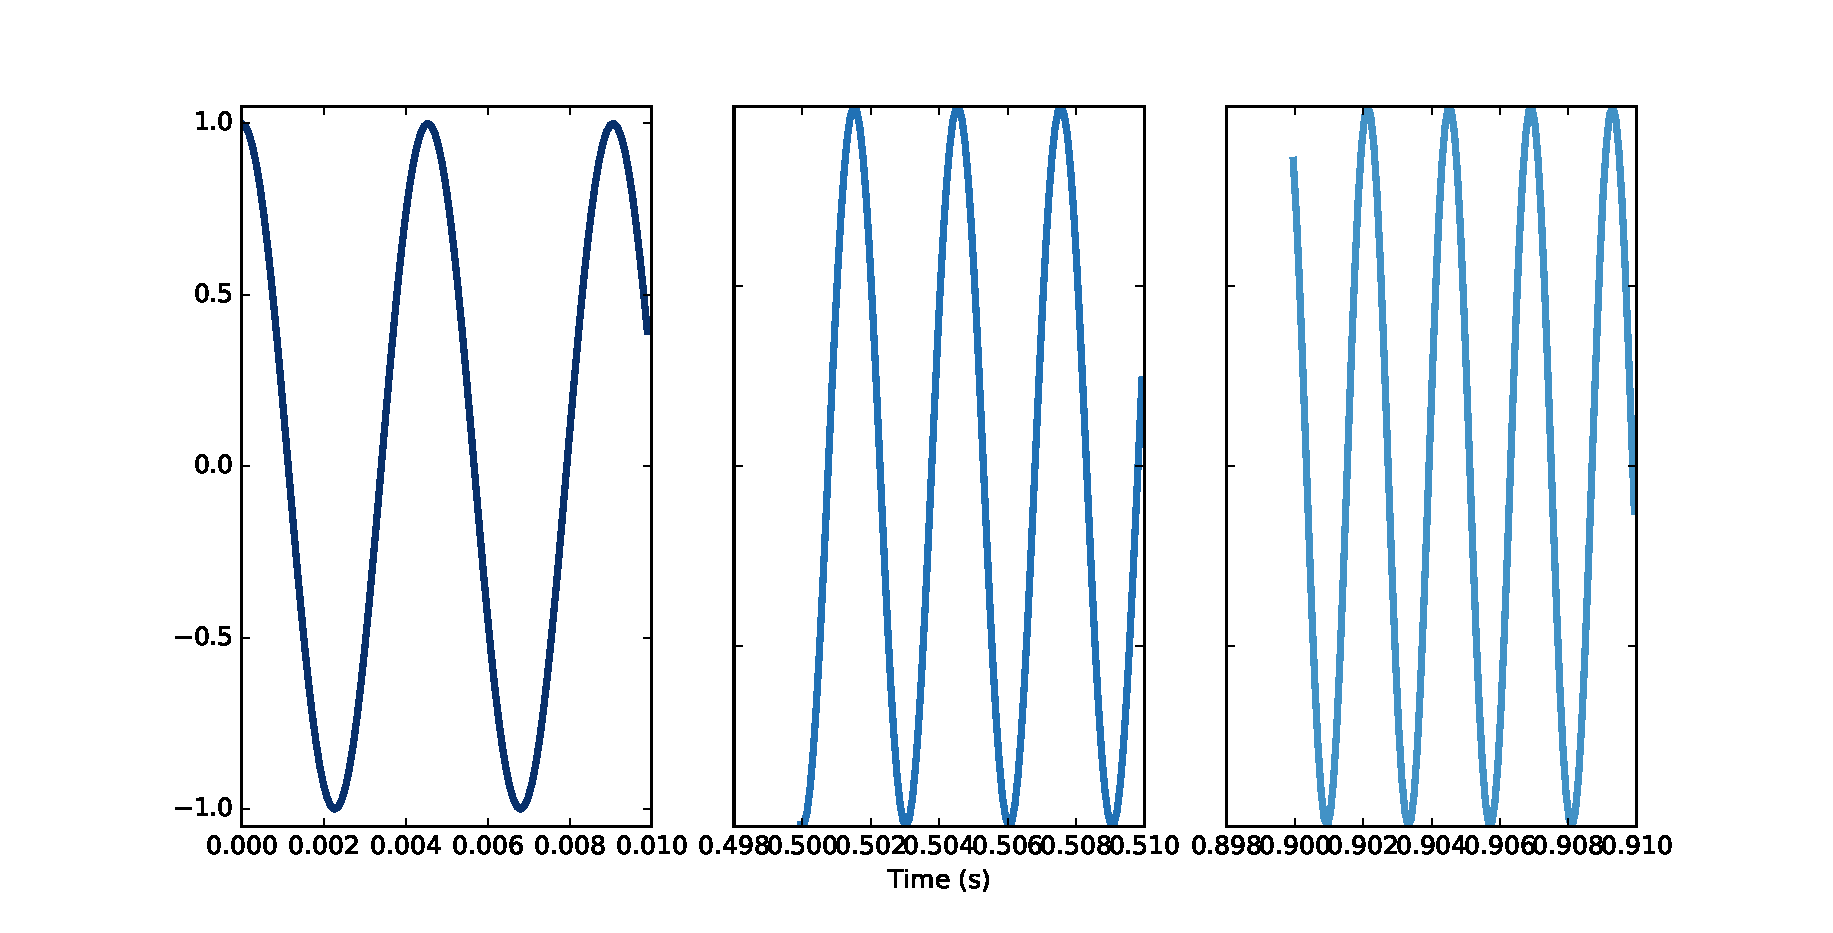
\includegraphics[height=2.5in]{figs/chirp3.eps}}
\caption{Chirp waveform near the beginning, middle, and end.}
\label{fig.chirp3}
\end{figure}

We'll start with a {\bf chirp}, which is a signal with variable
frequency.  {\tt thinkdsp} provides a Signal called Chirp that
makes a sinusoid that sweeps linearly through a range of
frequencies.

Here's an example what sweeps from 220 to 880 Hz, which
is two octaves from A3 to A5:

\begin{verbatim}
signal = thinkdsp.Chirp(start=220, end=880)
wave = signal.make_wave()
\end{verbatim}

Figure~\ref{fig.chirp3} shows segments of this wave near the
beginning, middle, and end.  It's clear that the frequency is
increasing.

Before we go on, let's see how Chirp is implemented.  Here
is the class definition:

\begin{verbatim}
class Chirp(Signal):
    
    def __init__(self, start=440, end=880, amp=1.0):
        self.start = start
        self.end = end
        self.amp = amp
\end{verbatim}

{\tt start} and {\tt end} are the frequencies, in Hz, at the start
and end of the chirp.  {\tt amp} is amplitude.

Here is the function that evaluates the signal:

\begin{verbatim}
    def evaluate(self, ts):
        freqs = np.linspace(self.start, self.end, len(ts)-1)
        return self._evaluate(ts, freqs)
\end{verbatim}

{\tt ts} is the sequence of points in time where the signal should be
evaluated; to keep this function simple, I assume they are equally-spaced.

If the length of {\tt ts} is $n$, you can think of it as a sequence of
$n-1$ intervals of time.  To compute the frequency during each
interval, I use {\tt np.linspace}, which returns a NumPy array of
$n-1$ values between {\tt start} and {\tt end}.

\verb"_evaluate" is a private method
that does the rest of the math\footnote{Beginning a method name
  with an underscore makes it ``private'', indicating that it is not
  part of the API that should be used outside the class definition.}:

\begin{verbatim}
    def _evaluate(self, ts, freqs):
        dts = np.diff(ts)
        dphis = PI2 * freqs * dts
        phases = np.cumsum(dphis)
        phases = np.insert(phases, 0, 0)
        ys = self.amp * np.cos(phases)
        return ys
\end{verbatim}

{\tt np.diff} computes the difference between adjacent elements
of {\tt ts}, returning the length of each interval in seconds.  
If the elements of {\tt ts} are equally spaced,
the {\tt dts} are all the same.

The next step is to figure out how much the phase changes during
each interval.  In Section~\ref{sigobs} we saw that when frequency is
constant, the phase, $\phi$, increases linearly over time:
%
\[ \phi = 2 \pi f t \]
%
When frequency is a function of time, the {\em change} in phase
during a short time interval, $\Delta t$ is:
%
\[ \Delta \phi = 2 \pi f(t) \Delta t \]
%
In Python, since {\tt freqs} contains $f(t)$ and {\tt dts}
contains the time intervals, we can write

\begin{verbatim}
dphis = PI2 * freqs * dts
\end{verbatim}

Now, since {\tt dphis} contains the changes in phase, we can
get the total phase at each timestep by adding up the changes:

\begin{verbatim}
phases = np.cumsum(dphis)
phases = np.insert(phases, 0, 0)
\end{verbatim}

{\tt np.cumsum} computes the cumulative sum, which is almost
what we want, but it doesn't start at 0.  So I use {\tt np.insert}
to add a 0 at the beginning.

The result is a NumPy array where the {\tt i}th element contains the
sum of the first {\tt i} terms from {\tt dphis}; that is, the total
phase at the end of the {\tt i}th interval.  Finally, {\tt np.cos}
computes the amplitude of the wave as a function of phase (remember
that phase is expressed in radians).

If you know calculus, you might notice that the limit as
$\Delta t$ gets small is
%
\[ d\phi = 2 \pi f(t) dt \]
%
Dividing through by $dt$ yields
%
\[ \frac{d\phi}{dt} = 2 \pi f(t) \]
%
In other words, frequency is the derivative of phase.  Conversely,
phase is the integral of frequency.  When we used {\tt cumsum}
to go from frequency to phase, we were approximating integration.


\section{Exponential chirp}

When you listen to this chirp, you might notice that the pitch
rises quickly at first and then slows down.
The chirp spans two octaves, but it only takes 2/3 s to span
the first octave, and twice as long to span the second.  

The reason is that our perception of pitch depends on the logarithm of
frequency.  As a result, the {\bf interval} we hear between two notes
depends on the {\em ratio} of their frequencies, not the difference.
``Interval'' is the musical term for the perceived difference between
two pitches.

For example, an octave is an interval where the ratio of two
pitches is 2.  So the interval from 220 to 440 is one octave
and the interval from 440 to 880 is also one octave.  The difference
in frequency is bigger, but the ratio is the same.

As a result, if frequency increases linearly, as in a linear
chirp, the perceived pitch increases logarithmically.

If you want the perceived pitch to increase linearly, the frequency
has to increase exponentially.  A signal with that shape is called
an {\bf exponential chirp}.

Here's the code that makes one:

\begin{verbatim}
class ExpoChirp(Chirp):
    
    def evaluate(self, ts):
        start, end = np.log10(self.start), np.log10(self.end)
        freqs = np.logspace(start, end, len(ts)-1)
        return self._evaluate(ts, freqs)
\end{verbatim}

Instead of {\tt np.linspace}, this version of evaluate uses
{\tt np.logspace}, which creates a series of frequencies
whose logarithms are equally spaced, which means that they increase
exponentially.

That's it; everything else is the same as Chirp.  Here's the code
that makes one:

\begin{verbatim}
    signal = thinkdsp.ExpoChirp(start=220, end=880)
    wave = signal.make_wave(duration=1)
\end{verbatim}

You can listen to these examples in {\tt chap03.ipynb} and compare
the linear and exponential chirps.  


\section{Spectrum of a chirp}
\label{sauron}

\begin{figure}
% chirp.py
\centerline{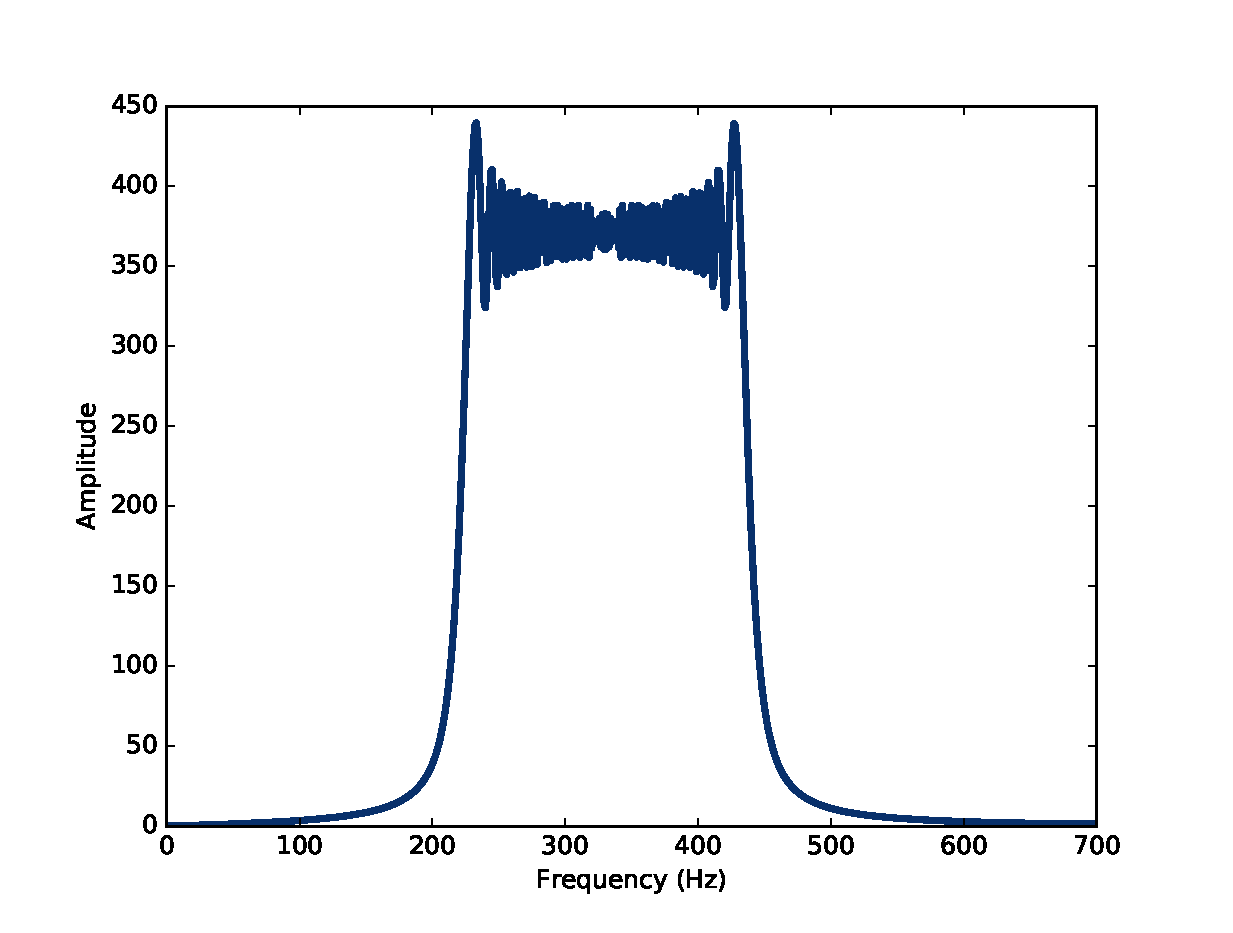
\includegraphics[height=2.5in]{figs/chirp1.eps}}
\caption{Spectrum of a one-second one-octave chirp.}
\label{fig.chirp1}
\end{figure}

What do you think happens if you compute the spectrum of a chirp?
Here's an example that constructs a one-second, one-octave chirp and
its spectrum:

\begin{verbatim}
    signal = thinkdsp.Chirp(start=220, end=440)
    wave = signal.make_wave(duration=1)
    spectrum = wave.make_spectrum()
\end{verbatim}

Figure~\ref{fig.chirp1} shows the result.  The spectrum has
components at every frequency from 220 to 440 Hz, with variations
that look a little like the Eye of Sauron
(see \url{http://en.wikipedia.org/wiki/Sauron}).

The spectrum is approximately flat between 220 and 440 Hz, which
indicates that the signal spends equal time at each frequency in this
range.  Based on that observation, you should be able to guess what
the spectrum of an exponential chirp looks like.

The spectrum gives hints about the structure of the signal,
but it obscures the relationship between frequency and time.
For example, we cannot tell by looking at this spectrum whether
the frequency went up or down, or both.


\section{Spectrogram}

\begin{figure}
% chirp.py
\centerline{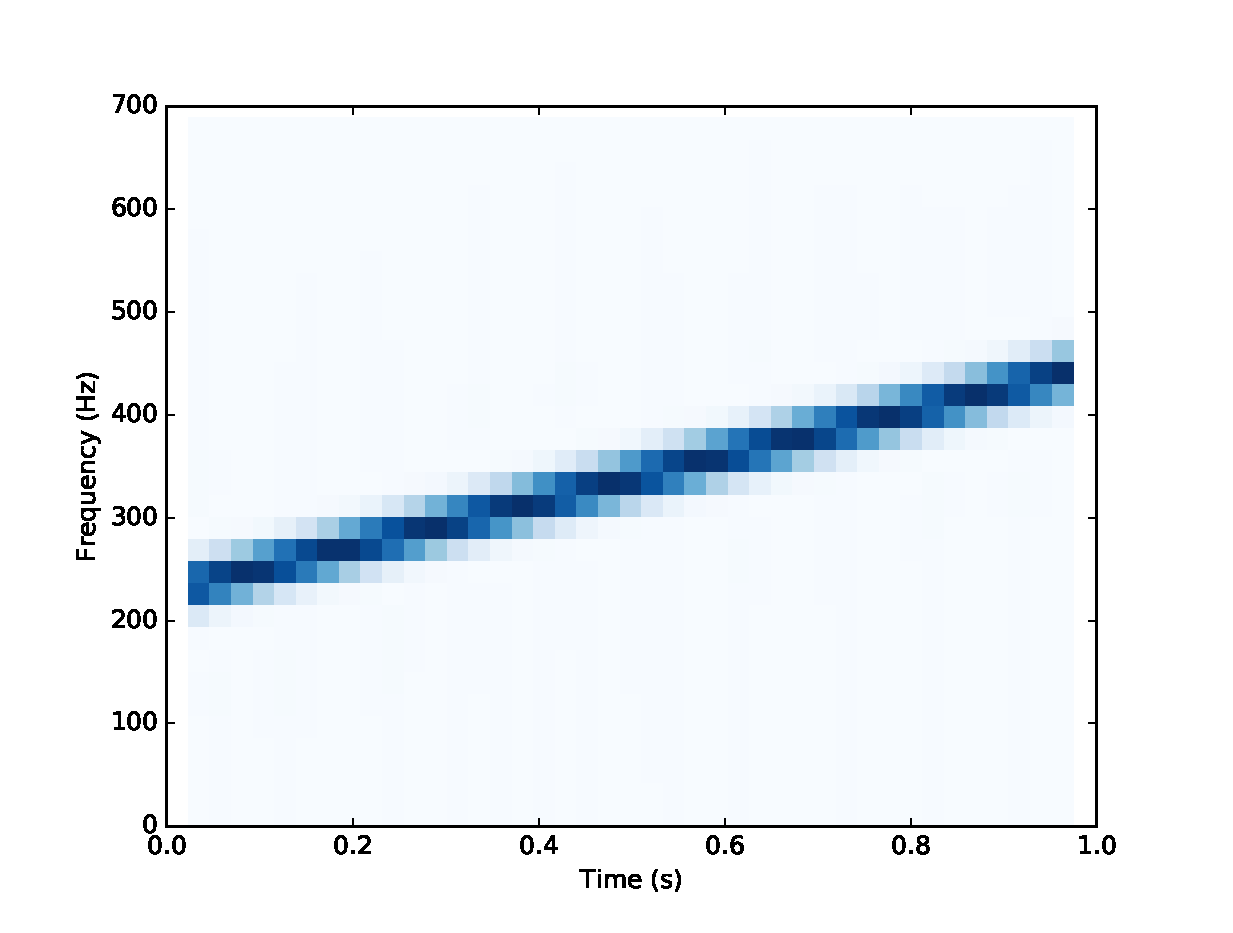
\includegraphics[height=2.5in]{figs/chirp2.eps}}
\caption{Spectrogram of a one-second one-octave chirp.}
\label{fig.chirp2}
\end{figure}

To recover the relationship between frequency and time, we can break
the chirp into segments and plot the spectrum of each segment.  The
result is called a {\bf short-time Fourier transform} (STFT).

There are several ways to visualize a STFT, but the most common
is a {\bf spectrogram}, which shows time on the x-axis and frequency
on the y-axis.  Each column in the spectrogram shows the spectrum of
a short segment, using color or grayscale to represent amplitude.

As an example, I'll compute the spectrogram of this chirp:

\begin{verbatim}
signal = thinkdsp.Chirp(start=220, end=440)
wave = signal.make_wave(duration=1, framerate=11025)
\end{verbatim}

{\tt Wave} provides \verb"make_spectrogram", which returns a
{\tt Spectrogram} object:

\begin{verbatim}
spectrogram = wave.make_spectrogram(seg_length=512)
spectrogram.plot(high=700)
\end{verbatim}

\verb"seg_length" is the number of samples in each segment.  I chose
512 because FFT is most efficient when the number of samples is a
power of 2.

Figure~\ref{fig.chirp2} shows the result.  The x-axis shows time from
0 to 1 seconds.  The y-axis shows frequency from 0 to 700 Hz.  I cut
off the top part of the spectrogram; the full range goes to 5512.5 Hz,
which is half of the framerate.

The spectrogram shows clearly that frequency increases linearly
over time.  Similarly, in the spectrogram of an exponential chirp, we
can see the shape of the exponential curve.

However, notice that the peak in each column is blurred across 2--3
cells.  This blurring reflects the limited resolution of the
spectrogram.


\section{The Gabor limit}
\label{gabor}

The {\bf time resolution} of the spectrogram is the duration of the
segments, which corresponds to the width of the cells in the
spectrogram.  Since each segment is 512 frames, and there are 11,025
frames per second, there are 0.046 seconds per segment.

The {\bf frequency resolution} is the frequency range between
elements in the spectrum, which corresponds to the height of the
cells.  With 512 frames, we get 256 frequency components over a range
from 0 to 5512.5 Hz, so the range between components is 21.6 Hz.

More generally, if $n$ is the segment length, the spectrum contains
$n/2$ components.  If the framerate is $r$, the maximum frequency in
the spectrum is $r/2$.  So the time resolution is $n/r$ and the
frequency resolution is
%
\[ \frac{r/2}{n/2} \]
%
which is $r/n$.

Ideally we would like time resolution to be small, so we can see rapid
changes in frequency.  And we would like frequency resolution to be
small so we can see small changes in frequency.  But you can't have
both.  Notice that time resolution, $n/r$, is the inverse of frequency
resolution, $r/n$.  So if one gets smaller, the other gets bigger.

For example, if you double the segment length, you cut frequency
resolution in half (which is good), but you double time resolution
(which is bad).  Even increasing the framerate doesn't help.  You get
more samples, but the range of frequencies increases at
the same time.

This tradeoff is called the {\bf Gabor limit} and it is a fundamental
limitation of this kind of time-frequency analysis.


\section{Leakage}

\begin{figure}
% chirp.py
\centerline{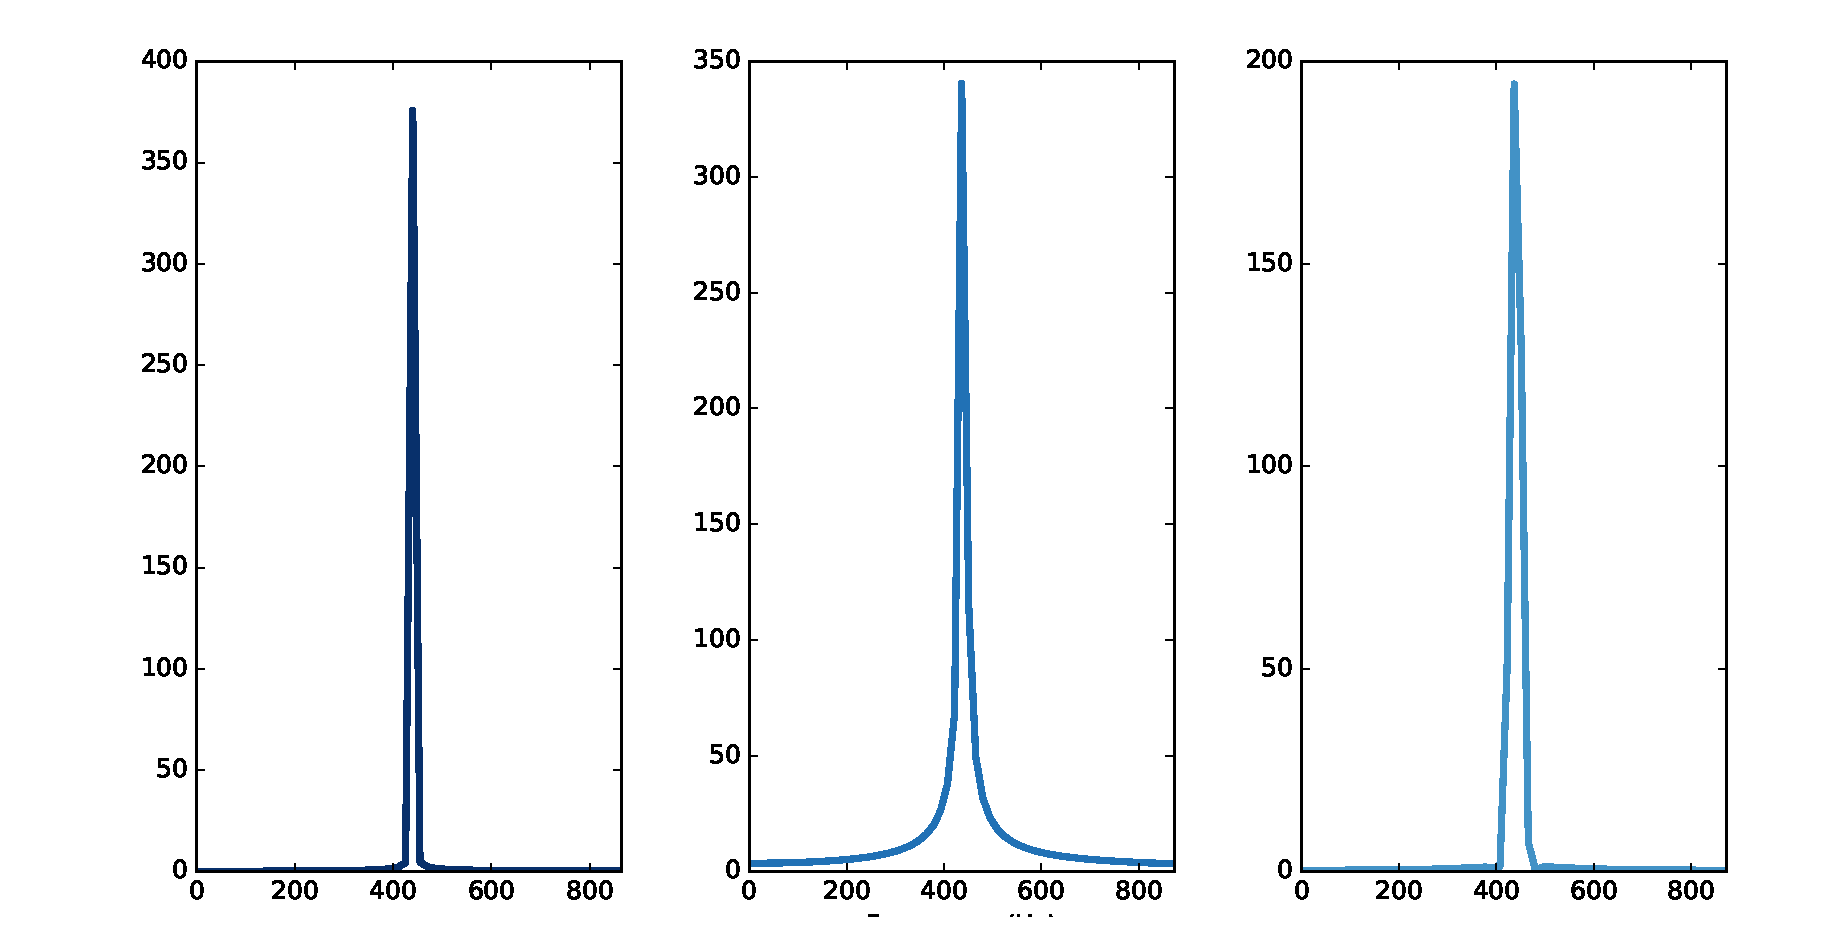
\includegraphics[height=2.5in]{figs/windowing1.eps}}
\caption{Spectrum of a periodic segment of a sinusoid (left), a
  non-periodic segment (middle), a windowed non-periodic segment
  (right).}
\label{fig.windowing1}
\end{figure}

In order to explain how \verb"make_spectrogram" works, I have
to explain windowing; and in order to explain windowing, I have to
show you the problem it is meant to address, which is leakage.

The Discrete Fourier Transform (DFT), which we use to compute
Spectrums, treats waves as if they are periodic; that is, it assumes
that the finite segment it operates on is a complete period from an
infinite signal that repeats over all time.  In practice, this
assumption is often false, which creates problems.

One common problem is discontinuity at the beginning and end of the
segment.  Because DFT assumes that the signal is periodic, it
implicitly connects the end of the segment back to the beginning to
make a loop.  If the end does not connect smoothly to the beginning,
the discontinuity creates additional frequency components in the
segment that are not in the signal.

As an example, let's start with a sine signal that contains only
one frequency component at 440 Hz.

\begin{verbatim}
    signal = thinkdsp.SinSignal(freq=440)
\end{verbatim}

If we select a segment that happens to be an integer multiple of
the period, the end of the segment connects smoothly with the
beginning, and DFT behaves well.

\begin{verbatim}
    duration = signal.period * 30
    wave = signal.make_wave(duration)
    spectrum = wave.make_spectrum()
\end{verbatim}

Figure~\ref{fig.windowing1} (left) shows the result.  As expected,
there is a single peak at 440 Hz.

But if the duration is not a multiple of the period, bad things
happen.  With {\tt duration = signal.period * 30.25}, the signal
starts at 0 and ends at 1.

Figure~\ref{fig.windowing1} (middle) shows
the spectrum of this segment.  Again, the peak is at 440 Hz, but now
there are additional components spread out from 240 to 640 Hz.  This
spread is called ``spectral leakage'', because some of the energy that
is actually at the fundamental frequency leaks into other frequencies.

In this example, leakage happens because we are using DFT on a segment
that becomes discontinuous when we treat it as periodic.


\section{Windowing}

\begin{figure}
% chirp.py
\centerline{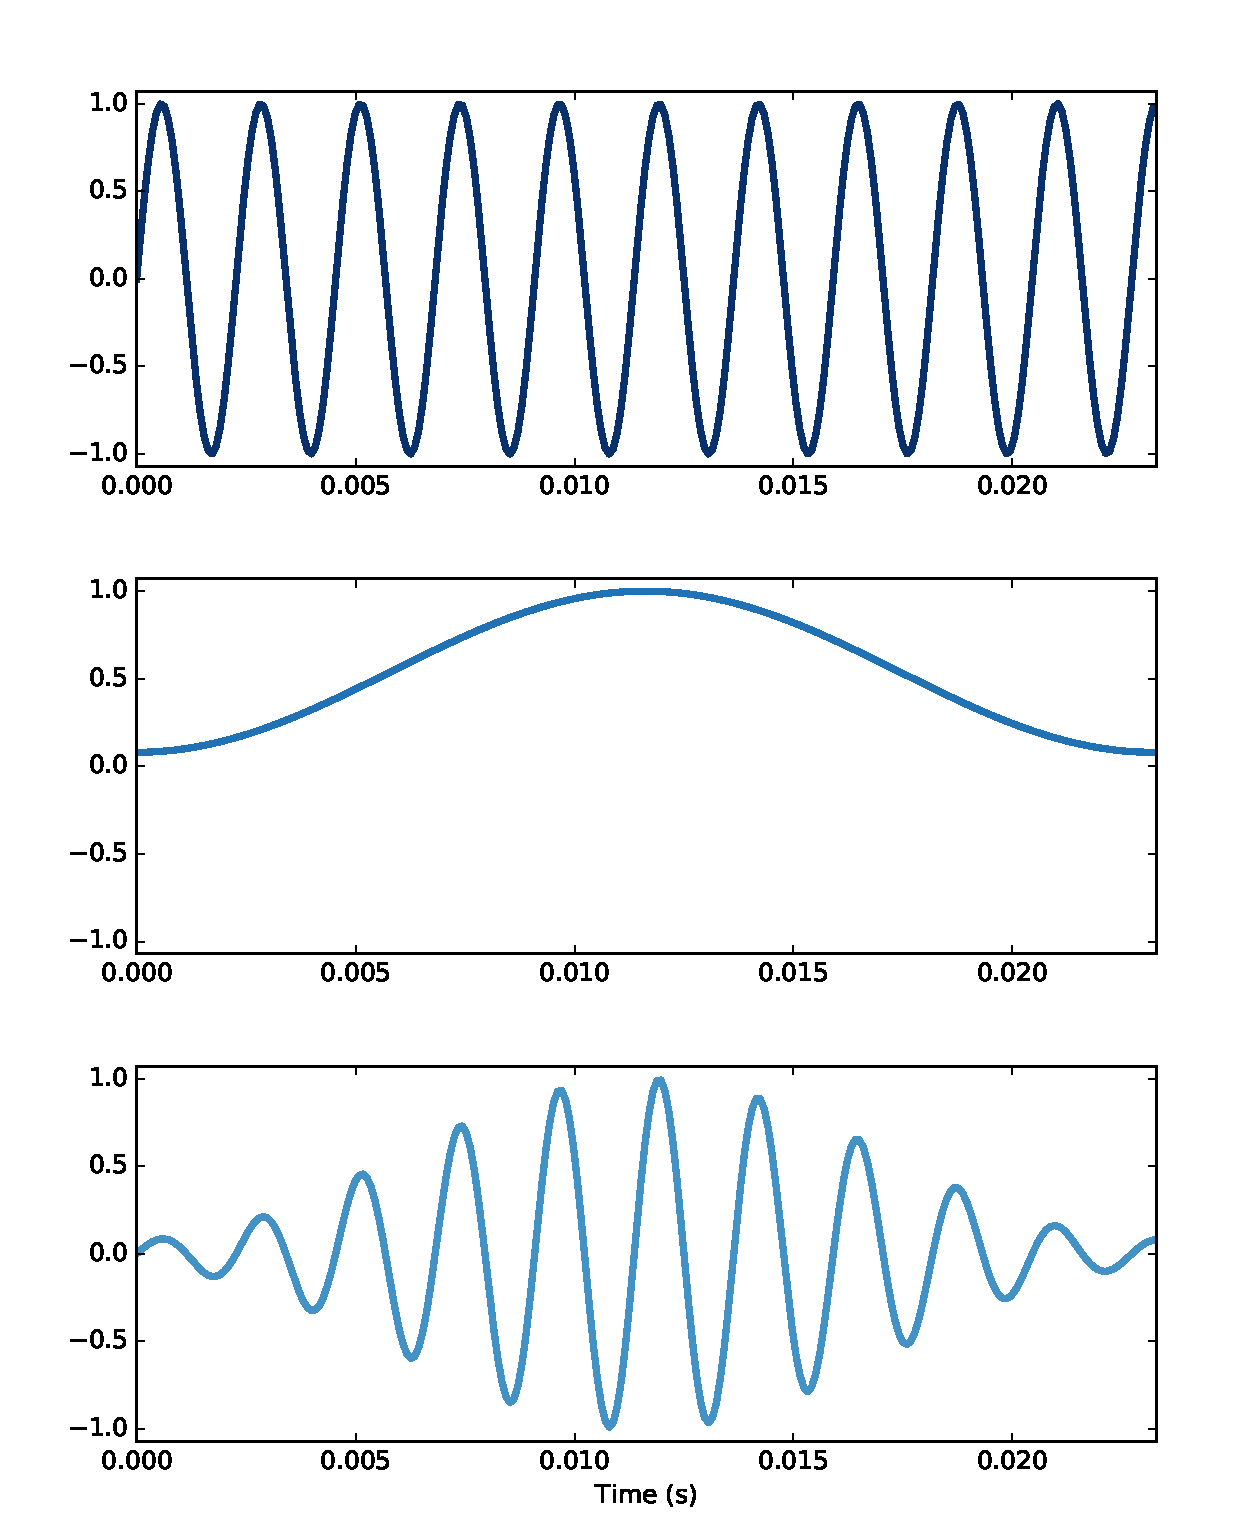
\includegraphics[height=3.5in]{figs/windowing2.eps}}
\caption{Segment of a sinusoid (top), Hamming window (middle), product
of the segment and the window (bottom).}
\label{fig.windowing2}
\end{figure}

We can reduce leakage by smoothing out the discontinuity between
the beginning and end of the segment, and one way to do that is
{\bf windowing}.

A ``window'' is a function designed to transform a non-periodic
segment into something that can pass for periodic.
Figure~\ref{fig.windowing2} (top) shows a segment where the end does not
connect smoothly to the beginning.

Figure~\ref{fig.windowing2} (middle) shows a ``Hamming window'', one of the
more common window functions.  No window function is perfect, but some
can be shown to be optimal for different applications, and Hamming
is a good, all-purpose window.

Figure~\ref{fig.windowing2} (bottom) shows the result of multiplying the
window by the original signal.  Where the window is close to 1, the
signal is unchanged.  Where the window is close to 0, the signal is
attenuated.  Because the window tapers at both ends, the end of the
segment connects smoothly to the beginning.

Figure~\ref{fig.windowing1} (right) shows the spectrum of the windowed
signal.  Windowing has reduced leakage substantially, but not
completely.

Here's what the code looks like.  {\tt Wave} provides {\tt window},
which applies a Hamming window:

\begin{verbatim}
#class Wave:
    def window(self, window):
        self.ys *= window
\end{verbatim}

And NumPy provides {\tt hamming}, which computes a Hamming window
with a given length:

\begin{verbatim}
window = np.hamming(len(wave))
wave.window(window)
\end{verbatim}

NumPy provides functions to compute other window
functions, including {\tt bartlett}, {\tt blackman}, {\tt hanning},
and {\tt kaiser}.  One of the exercises at the end of this chapter
asks you to experiment with these other windows.


\section{Implementing spectrograms}

\begin{figure}
% chirp.py
\centerline{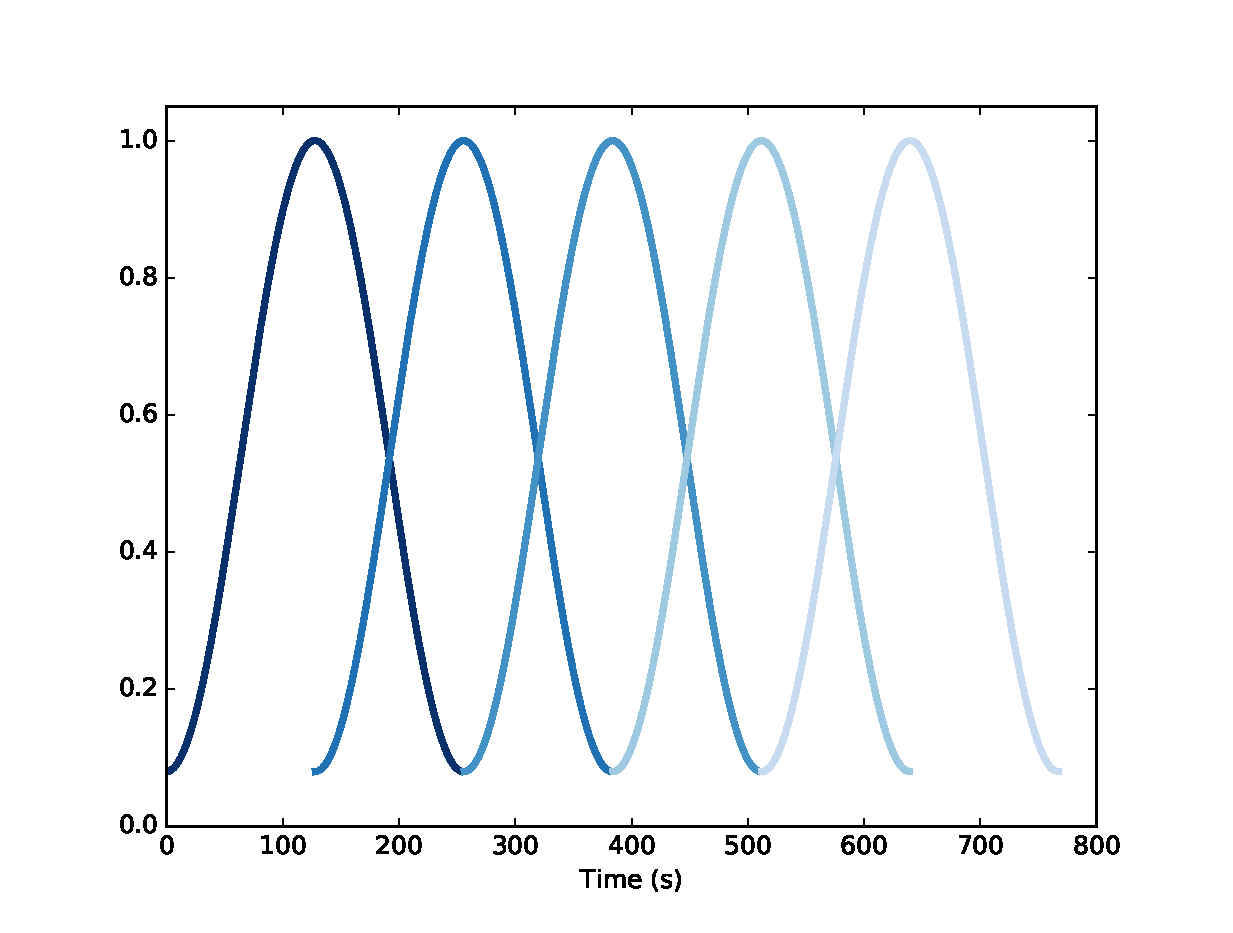
\includegraphics[height=2.5in]{figs/windowing3.eps}}
\caption{Overlapping Hamming windows.}
\label{fig.windowing3}
\end{figure}

Now that we understand windowing, we can understand the
implementation of spectrogram.
Here is the {\tt Wave} method that computes spectrograms:

\begin{verbatim}
#class Wave:
    def make_spectrogram(self, seg_length):
        window = np.hamming(seg_length)
        i, j = 0, seg_length
        step = seg_length / 2

        spec_map = {}

        while j < len(self.ys):
            segment = self.slice(i, j)
            segment.window(window)

            t = (segment.start + segment.end) / 2
            spec_map[t] = segment.make_spectrum()

            i += step
            j += step

        return Spectrogram(spec_map, seg_length)
\end{verbatim}

This is the longest function in the book, so if you can handle
this, you can handle anything.

The parameter, {\tt self}, is a Wave object.
\verb"seg_length" is the number of samples in each segment.

{\tt window} is a Hamming window with the same length as the segments.

{\tt i} and {\tt j} are the slice indices that select segments from
the wave.  {\tt step} is the offset between segments.  Since {\tt
  step} is half of \verb"seg_length", the segments overlap by half.
Figure~\ref{fig.windowing3} shows what these overlapping windows look
like.

\verb"spec_map" is a dictionary that maps from a timestamp to
a Spectrum.

Inside the while loop, we select a slice from the wave and apply
the window; then we construct a Spectrum
object and add it to \verb"spec_map".  The nominal time of
each segment, {\tt t}, is the midpoint.

Then we advance {\tt i} and {\tt j}, and continue as long as {\tt j}
doesn't go past the end of the Wave.

Finally, the method constructs and returns a Spectrogram.  Here
is the definition of Spectrogram:

\begin{verbatim}
class Spectrogram(object):
    def __init__(self, spec_map, seg_length):
        self.spec_map = spec_map
        self.seg_length = seg_length
\end{verbatim}

Like many init methods, this one just stores the
parameters as attributes.

{\tt Spectrogram} provides {\tt plot}, which generates a
pseudocolor plot with time along the x-axis and frequency along
the y-axis.

And that's how Spectrograms are implemented.


\section{Exercises}

Solutions to these exercises are in {\tt chap03soln.ipynb}.

\begin{exercise}
Run and listen to the examples in {\tt chap03.ipynb}, which is
in the repository for this book, and also available at
\url{http://tinyurl.com/thinkdsp03}.

In the leakage example, try replacing the Hamming window with one of
the other windows provided by NumPy, and see what effect they have on
leakage.  See
\url{http://docs.scipy.org/doc/numpy/reference/routines.window.html}
\end{exercise}


\begin{exercise}
Write a class called {\tt SawtoothChirp} that extends {\tt Chirp}
and overrides {\tt evaluate} to generate a sawtooth waveform with
frequency that increases (or decreases) linearly.

Hint: combine the evaluate functions from {\tt Chirp} and
{\tt SawtoothSignal}.

Draw a sketch of what you think the spectrogram of this signal
looks like, and then plot it.  The effect of aliasing should be
visually apparent, and if you listen carefully, you can hear it.
\end{exercise}


\begin{exercise}
Make a sawtooth chirp that sweeps from 2500 to 3000 Hz, then use it to
make a wave with duration 1 s and framerate 20 kHz.  Draw a sketch of
what you think the spectrum will look like.  Then plot the
spectrum and see if you got it right.
\end{exercise}


\begin{exercise}
In musical terminology, a ``glissando'' is a note that slides from one
pitch to another, so it is similar to a chirp.

Find or make a recording of a glissando and plot a spectrogram of the
first few seconds.  One suggestion: George Gershwin's {\it Rhapsody in
  Blue} starts with a famous clarinet glissando, which you can download
from \url{http://archive.org/details/rhapblue11924}.
\end{exercise}


\begin{exercise}
A trombone player can play a glissando by extending the trombone
slide while blowing continuously.  As the slide extends, the total
length of the tube gets longer, and the resulting pitch is inversely
proportional to length.

Assuming that the player moves the slide at a constant speed, how
does frequency vary with time?  

Write a class called {\tt TromboneGliss} that extends {\tt Chirp} and
provides {\tt evaluate}.  Make a wave that simulates a trombone
glissando from C3 up to F3 and back down to C3.  C3 is 262 Hz; F3 is
349 Hz.

Plot a spectrogram of the resulting wave.  Is a trombone glissando
more like a linear or exponential chirp?
\end{exercise}


\begin{exercise}
Make or find a recording of a series of vowel sounds and look at the
spectrogram.  Can you identify different vowels?
\end{exercise}


\chapter{Noise}

In English, ``noise'' means an unwanted or unpleasant sound.  In the
context of signal processing, it has two different senses:

\begin{enumerate}

\item As in English, it can mean an unwanted signal of any kind.  If
two signals interfere with each other, each signal would consider
the other to be noise.

\item ``Noise'' also refers to a signal that contains components at
many frequencies, so it lacks the harmonic structure of the periodic
signals we saw in previous chapters.  

\end{enumerate}

This chapter is about the second kind.

The code for this chapter is in {\tt chap04.ipynb}, which is in the
repository for this book (see Section~\ref{code}).
You can also view it at \url{http://tinyurl.com/thinkdsp04}.


\section{Uncorrelated noise}

\begin{figure}
% noise.py
\centerline{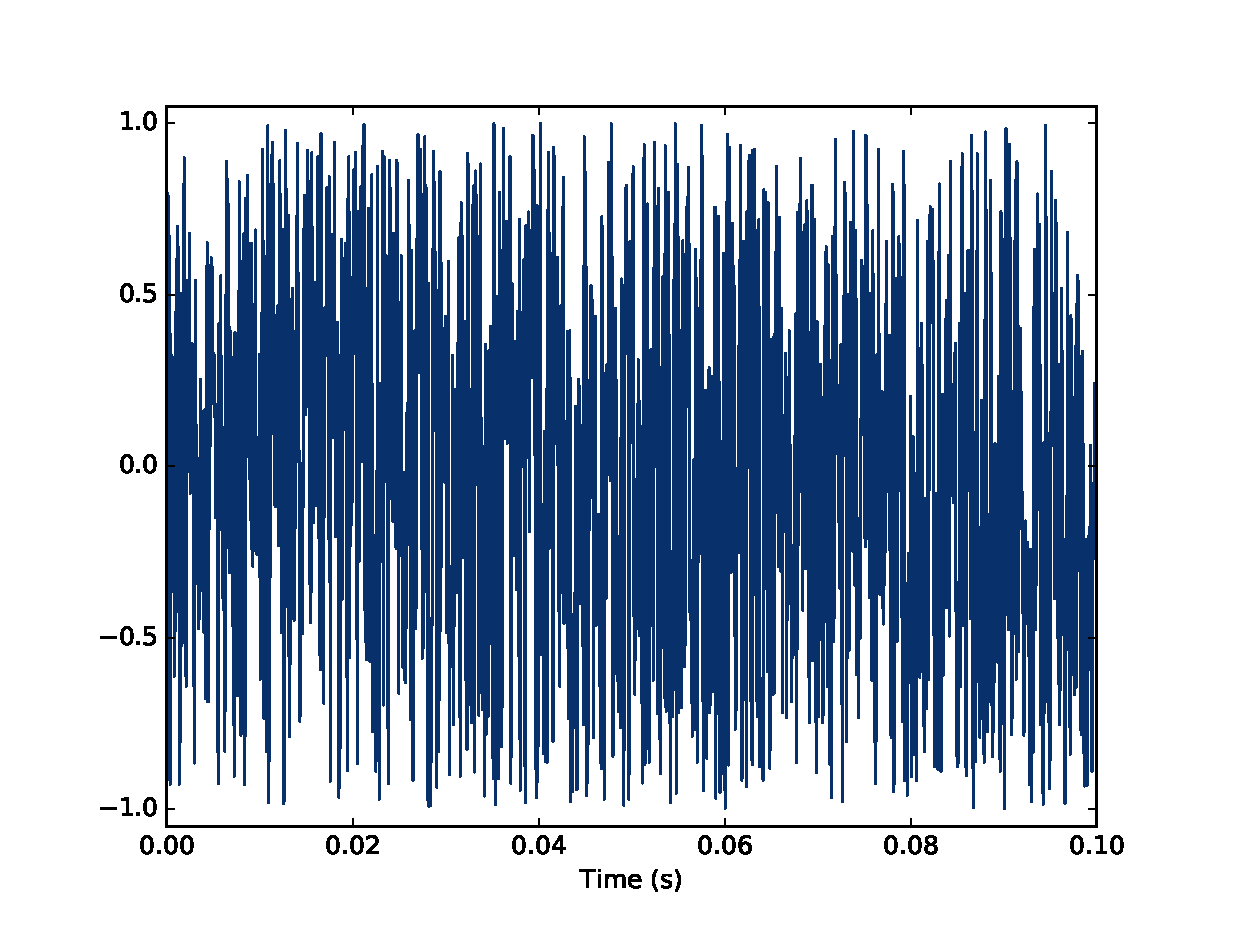
\includegraphics[height=2.5in]{figs/whitenoise0.eps}}
\caption{Waveform of uncorrelated uniform noise.}
\label{fig.whitenoise0}
\end{figure}

The simplest way to understand noise is to generate it, and the
simplest kind to generate is uncorrelated uniform noise (UU noise).
``Uniform'' means the signal contains random values from a uniform
distribution; that is, every value in the range is equally likely.
``Uncorrelated'' means that the values are independent; that is,
knowing one value provides no information about the others.

Here's a class that represents UU noise:

\begin{verbatim}
class UncorrelatedUniformNoise(_Noise):

    def evaluate(self, ts):
        ys = np.random.uniform(-self.amp, self.amp, len(ts))
        return ys
\end{verbatim}

{\tt UncorrelatedUniformNoise} inherits from \verb"_Noise", which
inherits from {\tt Signal}.

As usual, the evaluate function takes {\tt ts}, the times when the
signal should be evaluated.  It uses
{\tt np.random.uniform}, which generates values from a
uniform distribution.  In this example, the values are in
the range between {\tt -amp} to {\tt amp}.

The following example generates UU noise with duration 0.5
seconds at 11,025 samples per second.

\begin{verbatim}
signal = thinkdsp.UncorrelatedUniformNoise()
wave = signal.make_wave(duration=0.5, framerate=11025)
\end{verbatim}

If you play this wave, it sounds like the static you hear if you tune
a radio between channels.  Figure~\ref{fig.whitenoise0} shows what the
waveform looks like.  As expected, it looks pretty random.

\begin{figure}
% noise.py
\centerline{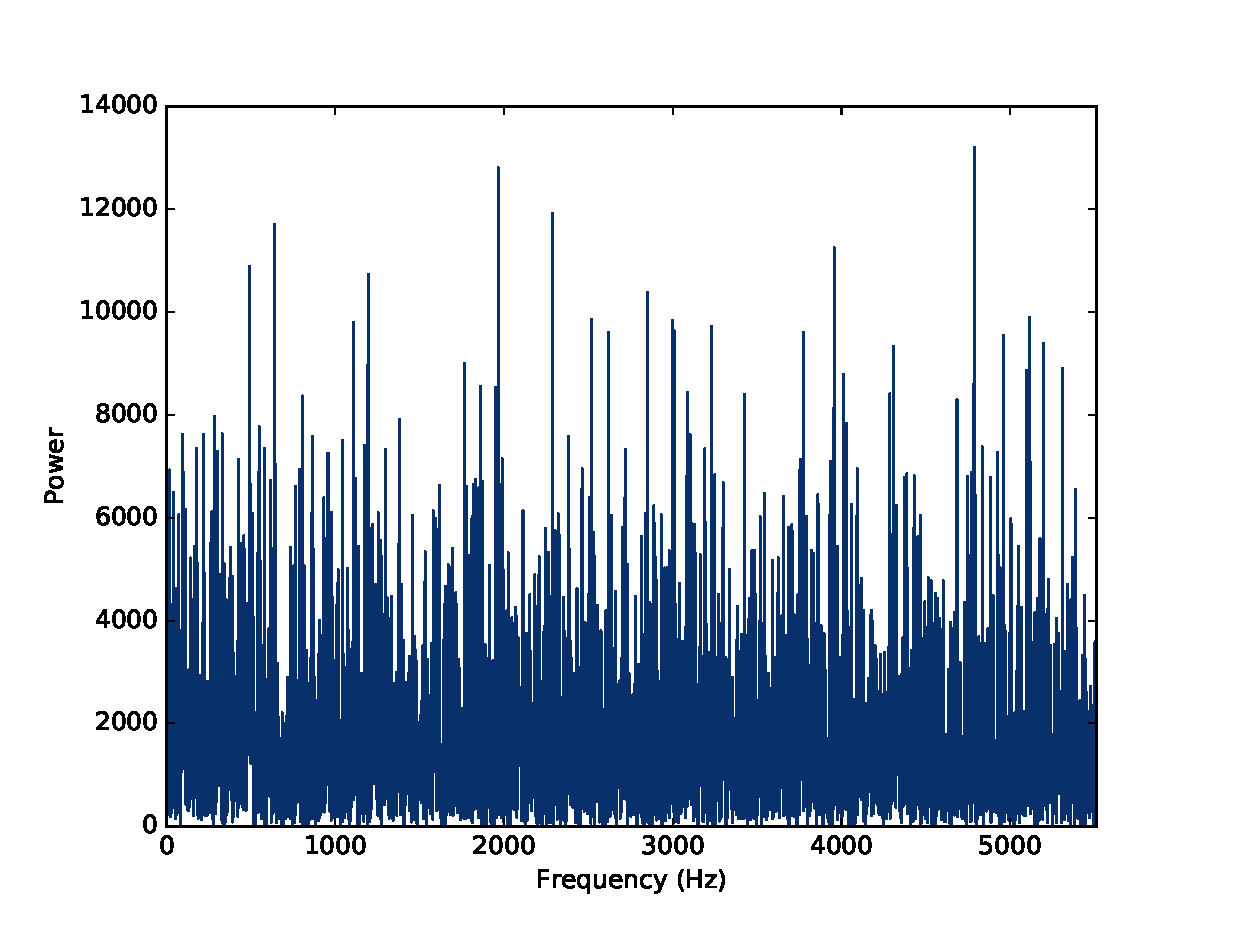
\includegraphics[height=2.5in]{figs/whitenoise1.eps}}
\caption{Power spectrum of uncorrelated uniform noise.}
\label{fig.whitenoise1}
\end{figure}

Now let's take a look at the spectrum:

\begin{verbatim}
spectrum = wave.make_spectrum()
spectrum.plot_power()
\end{verbatim}

\verb"Spectrum.plot_power" is similar to \verb"Spectrum.plot",
except that it plots power instead of amplitude.
Power is the square of amplitude.
I am switching from amplitude to power in this chapter because
it is more conventional in the context of noise.

Figure~\ref{fig.whitenoise1} shows the result.  Like the signal, the
spectrum looks pretty random.  In fact, it {\em is} random, but we have to
be more precise about the word ``random''.  There are at least three
things we might like to know about a noise signal or its spectrum:

\begin{itemize}

\item Distribution: The distribution of a random signal is the set of
  possible values and their probabilities.  For example, in the
  uniform noise signal, the set of values is the range from -1 to 1,
  and all values have the same probability.  An alternative is
  {\bf Gaussian noise}, where the set of values is the range from negative
  to positive infinity, but values near 0 are the most likely, with
  probability that drops off according to the Gaussian or
  ``bell'' curve.

\item Correlation: Is each value in the signal independent of the
  others, or are there dependencies between them?  In UU noise, the
  values are independent.
  An alternative is {\bf Brownian noise}, where each value is the sum
  of the previous value and a random ``step''.  So if the value of the
  signal is high at a particular point in time, we expect it to stay
  high, and if it is low, we expect
  it to stay low.

\item Relationship between power and frequency: In the spectrum of UU
  noise, the power at all frequencies is drawn from the same
  distribution; that is, the average power is the same for all
  frequencies.  An alternative is {\bf pink noise}, where power is
  inversely related to frequency; that is, the power at frequency $f$
  is drawn from a distribution whose mean is proportional to $1/f$.

\end{itemize}


\section{Integrated spectrum}

For UU noise we can see the relationship between power and frequency
more clearly by looking at the {\bf integrated spectrum}, which
is a function of frequency, $f$, that shows the cumulative power in
the spectrum up to $f$.

\begin{figure}
% noise.py
\centerline{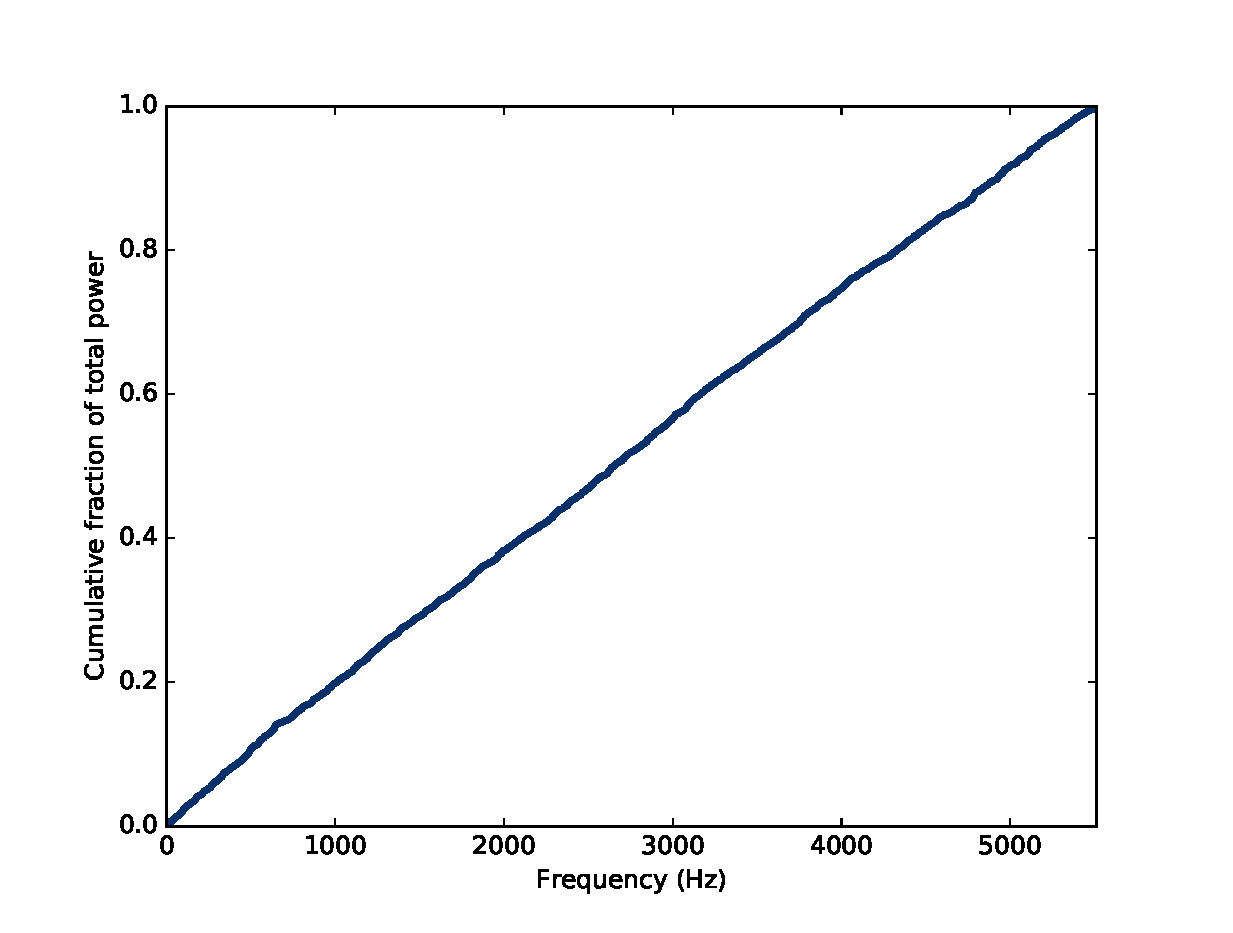
\includegraphics[height=2.5in]{figs/whitenoise2.eps}}
\caption{Integrated spectrum of uncorrelated uniform noise.}
\label{fig.whitenoise2}
\end{figure}

{\tt Spectrum} provides a method that computes the IntegratedSpectrum:

\begin{verbatim}
    def make_integrated_spectrum(self):
        cs = np.cumsum(self.power)
        cs /= cs[-1]
        return IntegratedSpectrum(cs, self.fs)
\end{verbatim}

{\tt self.power} is a NumPy array containing power for each frequency.
{\tt np.cumsum} computes the cumulative sum of the powers.
Dividing through by the last element normalizes the integrated
spectrum so it runs from 0 to 1.

The result is an IntegratedSpectrum.  Here is the class definition:

\begin{verbatim}
class IntegratedSpectrum(object):    
    def __init__(self, cs, fs):
        self.cs = cs
        self.fs = fs
\end{verbatim}

Like Spectrum, IntegratedSpectrum provides \verb"plot_power", so
we can compute and plot the integrated spectrum like this:

\begin{verbatim}
    integ = spectrum.make_integrated_spectrum()
    integ.plot_power()
\end{verbatim}

The result, shown in Figure~\ref{fig.whitenoise2}, is a straight line,
which indicates that power at all frequencies is constant, on average.
Noise with equal power at all frequencies is called {\bf white noise}
by analogy with light, because an equal mixture of light at all
visible frequencies is white.



\section{Brownian noise}
\label{brownian}

\begin{figure}
% noise.py
\centerline{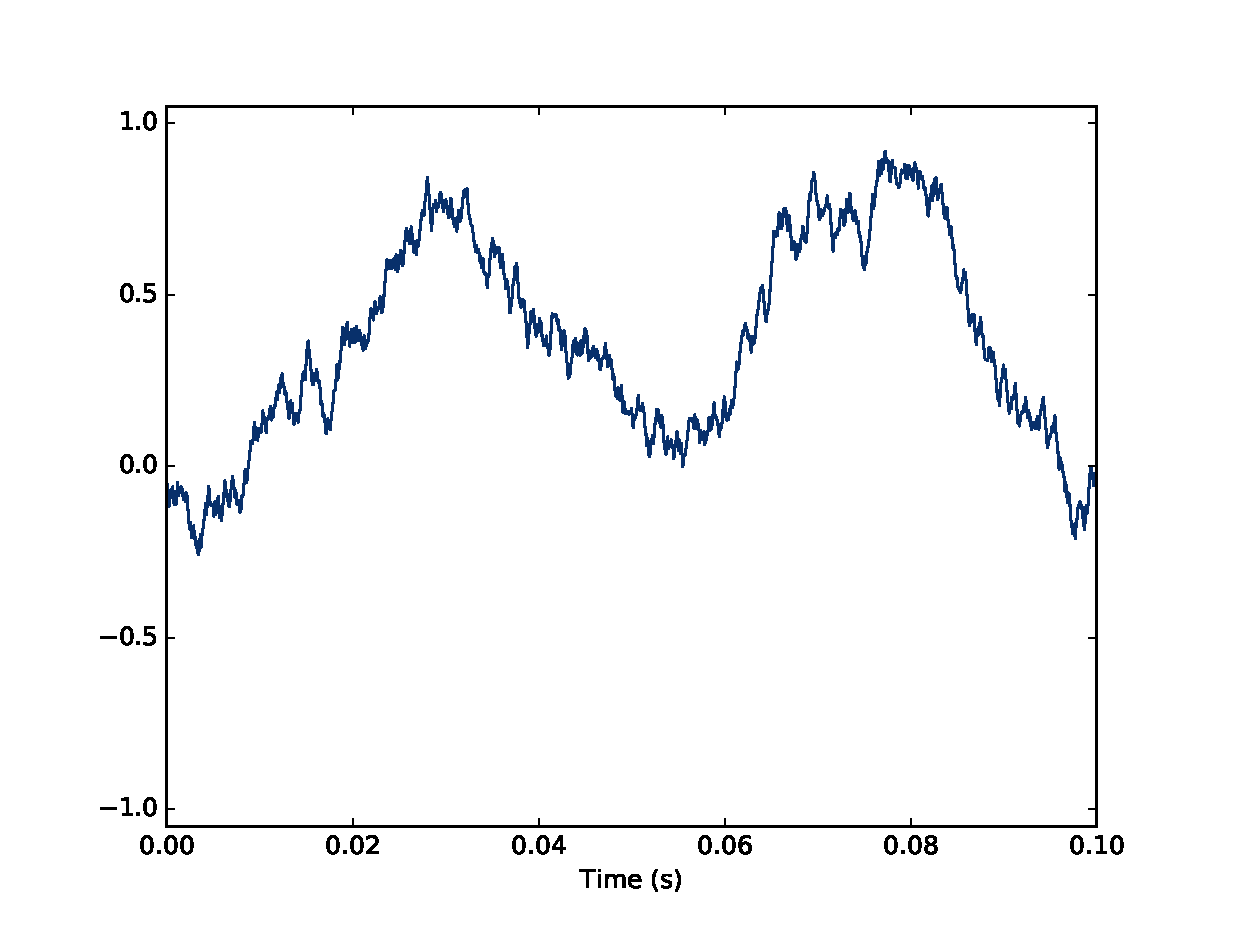
\includegraphics[height=2.5in]{figs/rednoise0.eps}}
\caption{Waveform of Brownian noise.}
\label{fig.rednoise0}
\end{figure}

UU noise is uncorrelated, which means that each value does not depend
on the others.  An alternative is Brownian noise, in which each value
is the sum of the previous value and a random ``step''.

It is called ``Brownian'' by analogy with Brownian motion, in which a
particle suspended in a fluid moves apparently at random, due to
unseen interactions with the fluid.  Brownian motion is often
described using a {\bf random walk}, which is a mathematical model 
of a path where the distance between steps is characterized by a
random distribution.

In a one-dimensional random walk, the particle moves up or down
by a random amount at each time step.  The location of the particle
at any point in time is the sum of all previous steps.

This observation suggests a way to generate Brownian noise:
generate uncorrelated random steps and then add them up.
Here is a class definition that implements this algorithm:

\begin{verbatim}
class BrownianNoise(_Noise):

    def evaluate(self, ts):
        dys = np.random.uniform(-1, 1, len(ts))
        ys = np.cumsum(dys)
        ys = normalize(unbias(ys), self.amp)
        return ys
\end{verbatim}

{\tt evaluate} uses {\tt np.random.uniform} to generate an
uncorrelated signal and {\tt np.cumsum} to compute their cumulative
sum.

Since the sum is likely to escape the range from -1 to
1, we have to use {\tt unbias} to shift the mean to 0, and {\tt
  normalize} to get the desired maximum amplitude.

Here's the code that generates a BrownianNoise object and plots the
waveform.

\begin{verbatim}
    signal = thinkdsp.BrownianNoise()
    wave = signal.make_wave(duration=0.5, framerate=11025)
    wave.plot()
\end{verbatim}

Figure~\ref{fig.rednoise0} shows the result.  The waveform
wanders up and down, but there is a clear correlation between
successive values.  When the amplitude is high, it tends to stay
high, and vice versa.

\begin{figure}
% noise.py
\centerline{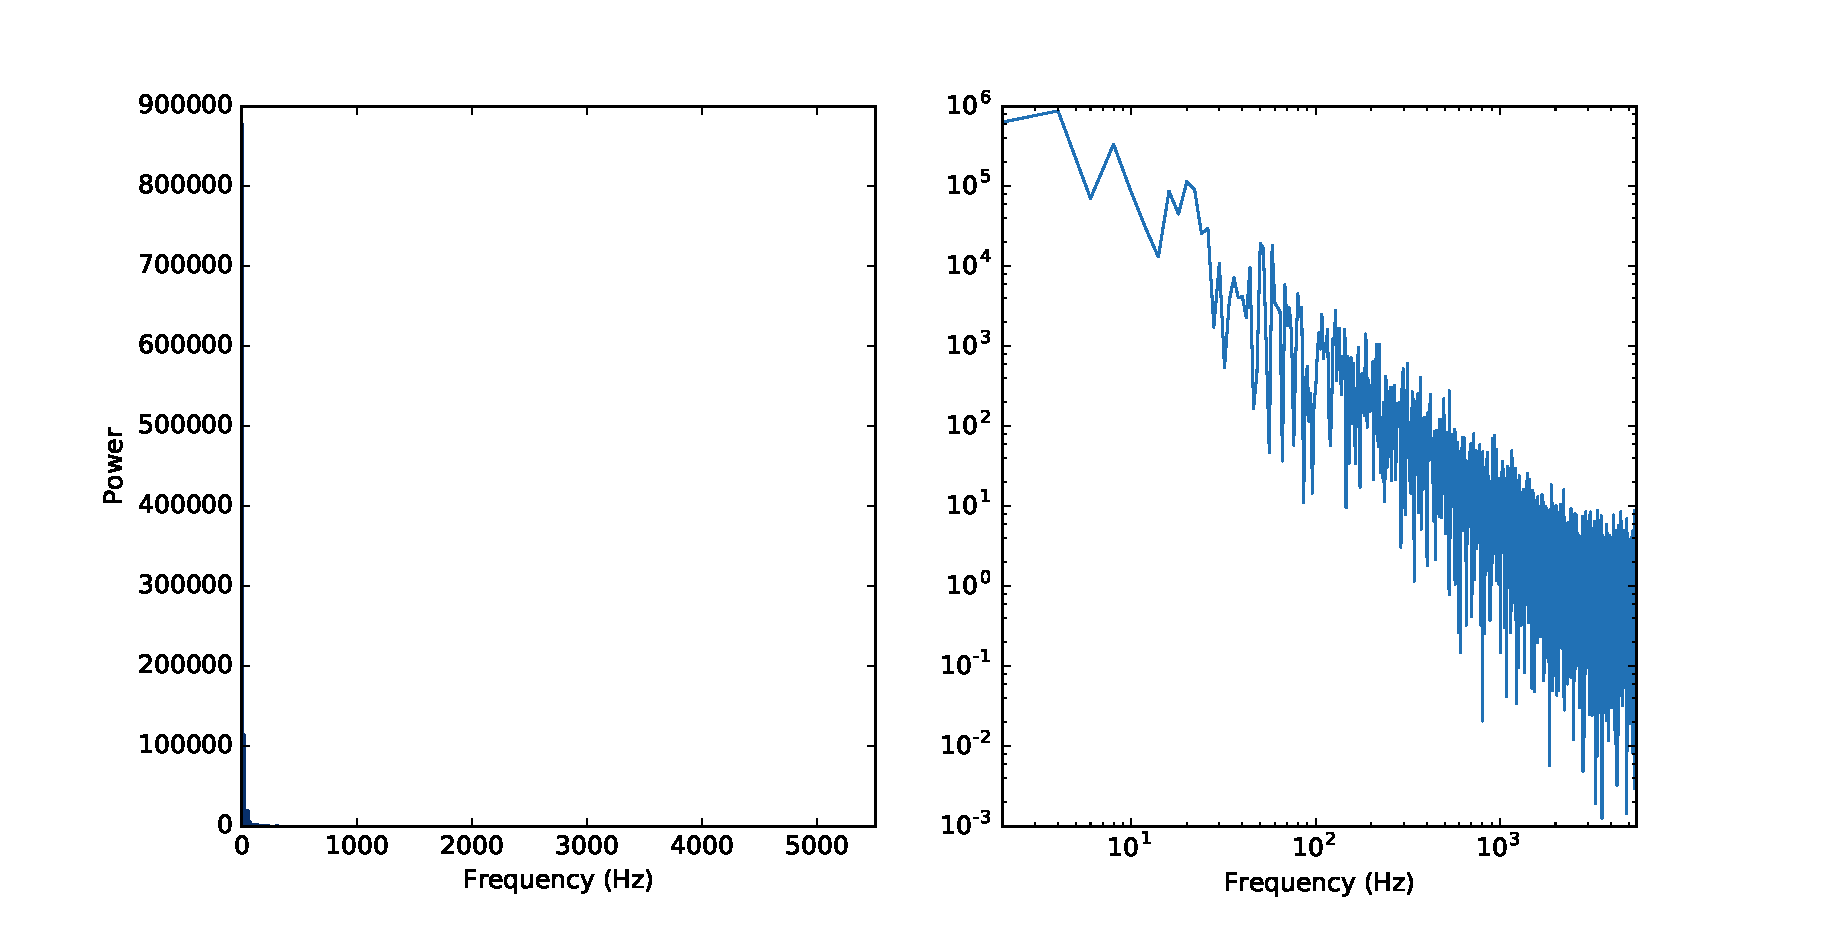
\includegraphics[height=2.5in]{figs/rednoise3.eps}}
\caption{Spectrum of Brownian noise on a log-log scale.}
\label{fig.rednoise3}
\end{figure}

If you plot the spectrum of Brownian noise, it doesn't look like
much.  Nearly all of the power is at the lowest frequencies; on a
linear scale, the higher frequency components are not visible.

To see the shape of the spectrum more clearly, we can plot power
and frequency on a log-log scale.  Here's the code:

\begin{verbatim}
    spectrum = wave.make_spectrum()
    spectrum.plot_power(linewidth=1, alpha=0.5)
    thinkplot.config(xscale='log', yscale='log')
\end{verbatim}

The result is in Figure~\ref{fig.rednoise3}.  The relationship between
power and frequency is noisy, but roughly linear.

{\tt Spectrum} provides \verb"estimate_slope", which uses SciPy to compute
a least squares fit to the power spectrum:

\begin{verbatim}
#class Spectrum

    def estimate_slope(self):
        x = np.log(self.fs[1:])
        y = np.log(self.power[1:])
        t = scipy.stats.linregress(x,y)
        return t
\end{verbatim}

It discards the first component of the spectrum because
this component corresponds to $f=0$, and $\log 0$ is undefined.

\verb"estimate_slope" returns the result from {\tt
  scipy.stats.linregress} which is an object that contains the
estimated slope and intercept, coefficient of determination ($R^2$),
p-value, and standard error.  For our purposes, we only need the
slope.

For Brownian noise, the slope of the power spectrum is -2 (we'll see
why in Chapter~\ref{diffint}), so we can write this relationship:
%
\[ \log P = k -2 \log f \]
%
where $P$ is power, $f$ is frequency, and $k$ is the intercept
of the line, which is not important for our purposes.
Exponentiating both sides yields:
%
\[ P = K / f^{2} \]
%
where $K$ is $e^k$, but still not important.  More relevant is
that power is proportional to $1/f^2$, which is characteristic
of Brownian noise.

Brownian noise is also called {\bf red noise}, for the same reason that
white noise is called ``white''.  If you combine visible light with
power proportional to $1/f^2$, most of the power
would be at the low-frequency end of the spectrum, which is red.
Brownian noise is also sometimes called ``brown noise'', but I think
that's confusing, so I won't use it.

%TODO: refer back to this in the diff/int chapter


\section{Pink Noise}
\label{pink}

\begin{figure}
% noise.py
\centerline{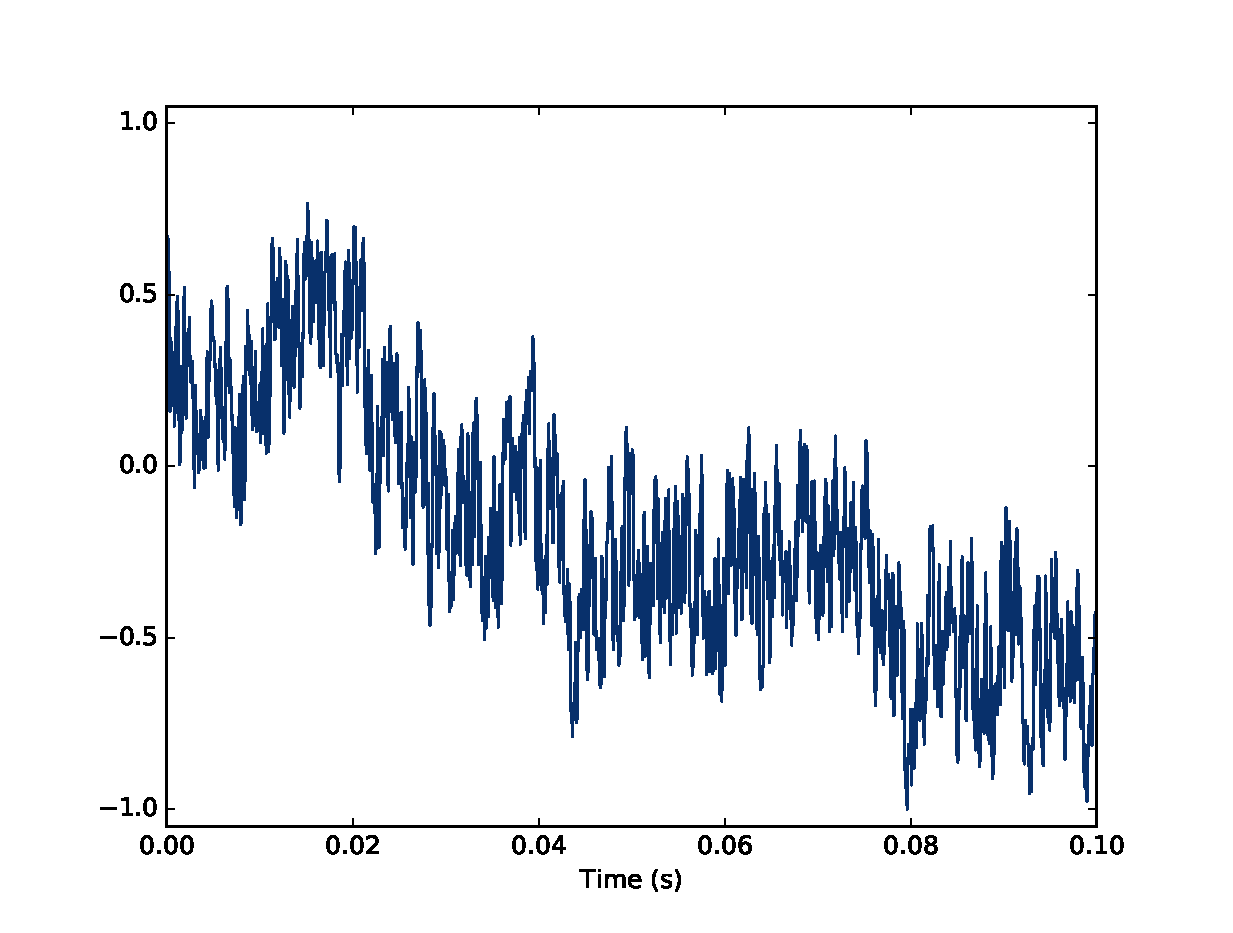
\includegraphics[height=2.5in]{figs/pinknoise0.eps}}
\caption{Waveform of pink noise with $\beta=1$.}
\label{fig.pinknoise0}
\end{figure}

For red noise, the relationship between frequency
and power is
%
\[ P = K / f^{2} \]
%
There is nothing special about the exponent 2.  More generally,
we can synthesize noise with any exponent, $\beta$.
%
\[ P = K / f^{\beta} \]
%
When $\beta = 0$, power is constant at all frequencies,
so the result is white noise.  When $\beta=2$ the result is red noise.

When $\beta$ is between 0 and 2, the result is between white and
red noise, so it is called ``pink noise''.

There are several ways to generate pink noise.  The simplest is to
generate white noise and then apply a low-pass filter with the
desired exponent.  {\tt thinkdsp} provides a class that represents
a pink noise signal:

\begin{verbatim}
class PinkNoise(_Noise):

    def __init__(self, amp=1.0, beta=1.0):
        self.amp = amp
        self.beta = beta
\end{verbatim}

{\tt amp} is the desired amplitude of the signal.
{\tt beta} is the desired exponent.  {\tt PinkNoise} provides
\verb"make_wave", which generates a Wave.

\begin{verbatim}
    def make_wave(self, duration=1, start=0, framerate=11025):
        signal = UncorrelatedUniformNoise()
        wave = signal.make_wave(duration, start, framerate)
        spectrum = wave.make_spectrum()

        spectrum.pink_filter(beta=self.beta)

        wave2 = spectrum.make_wave()
        wave2.unbias()
        wave2.normalize(self.amp)
        return wave2
\end{verbatim}

{\tt duration} is the length of the wave in seconds.  {\tt start} is
the start time of the wave; it is included so that \verb"make_wave"
has the same interface for all types of signal, but for random noise,
start time is irrelevant.  And {\tt framerate} is the number of
samples per second.

\begin{figure}
% noise.py
\centerline{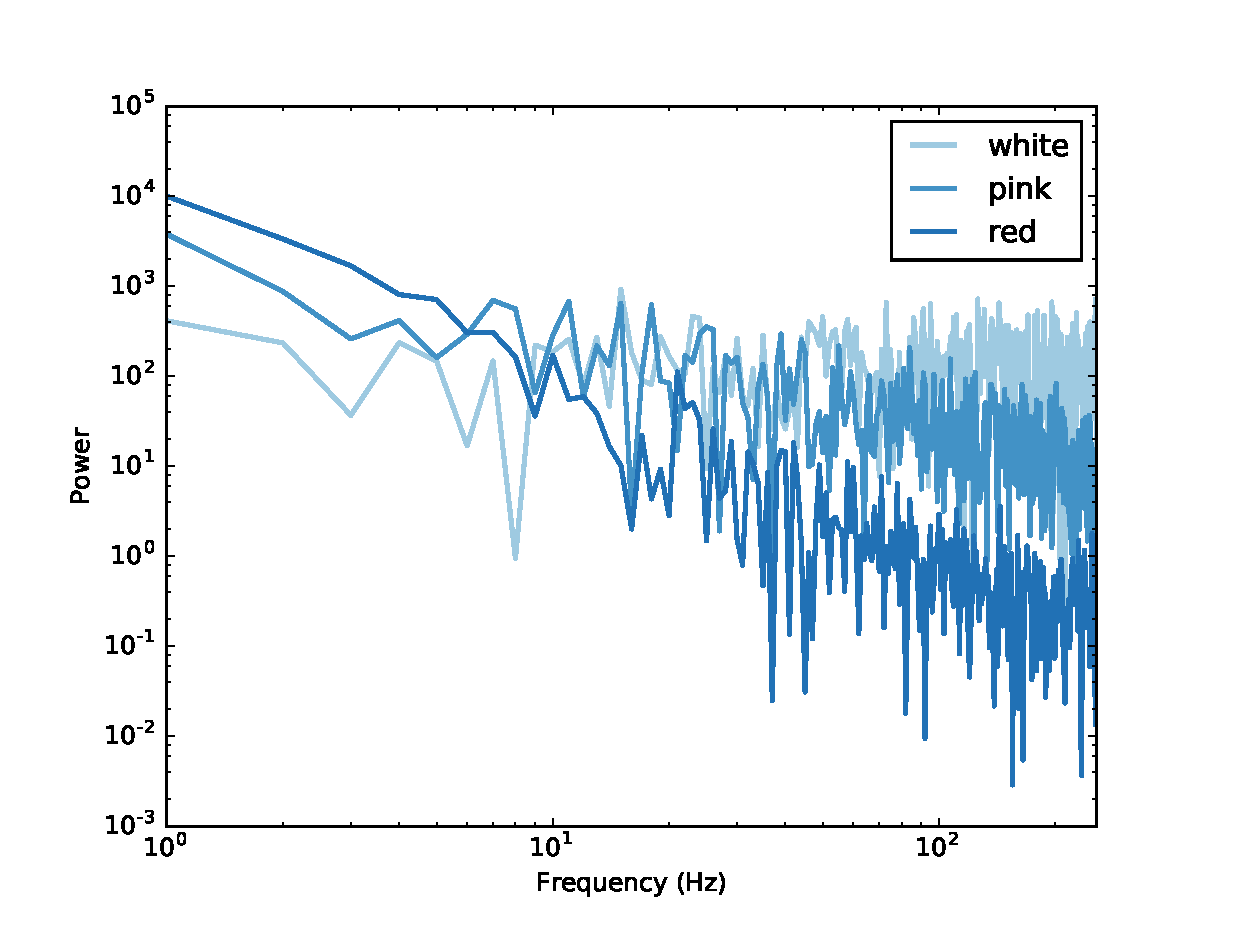
\includegraphics[height=2.5in]{figs/noise-triple.eps}}
\caption{Spectrum of white, pink, and red noise on a log-log scale.}
\label{fig.noise-triple}
\end{figure}

\verb"make_wave" creates a white noise wave, computes its spectrum,
applies a filter with the desired exponent, and then converts the
filtered spectrum back to a wave.  Then it unbiases and normalizes
the wave.

{\tt Spectrum} provides \verb"pink_filter":

\begin{verbatim}
    def pink_filter(self, beta=1.0):
        denom = self.fs ** (beta/2.0)
        denom[0] = 1
        self.hs /= denom
\end{verbatim}

\verb"pink_filter" divides each element of the spectrum by
$f^{\beta/2}$.  Since power is the square of amplitude, this
operation divides the power at
each component by $f^\beta$.  It treats the component
at $f=0$ as a special case, partly to avoid dividing by 0, and partly
because this element represents the bias of the signal,
which we are going to set to 0 anyway. 

Figure~\ref{fig.pinknoise0} shows the resulting waveform.  Like
Brownian noise, it wanders up and down in a way that suggests
correlation between successive values, but at least visually, it looks
more random.  In the next chapter we will come back to this
observation and I will be more precise about what I mean by
``correlation'' and ``more random''.

Finally, Figure~\ref{fig.noise-triple} shows a spectrum for
white, pink, and red noise on the same log-log scale.
The relationship between the exponent, $\beta$, and the slope
of the spectrum is apparent in this figure.


\section{Gaussian noise}

\begin{figure}
% noise.py
\centerline{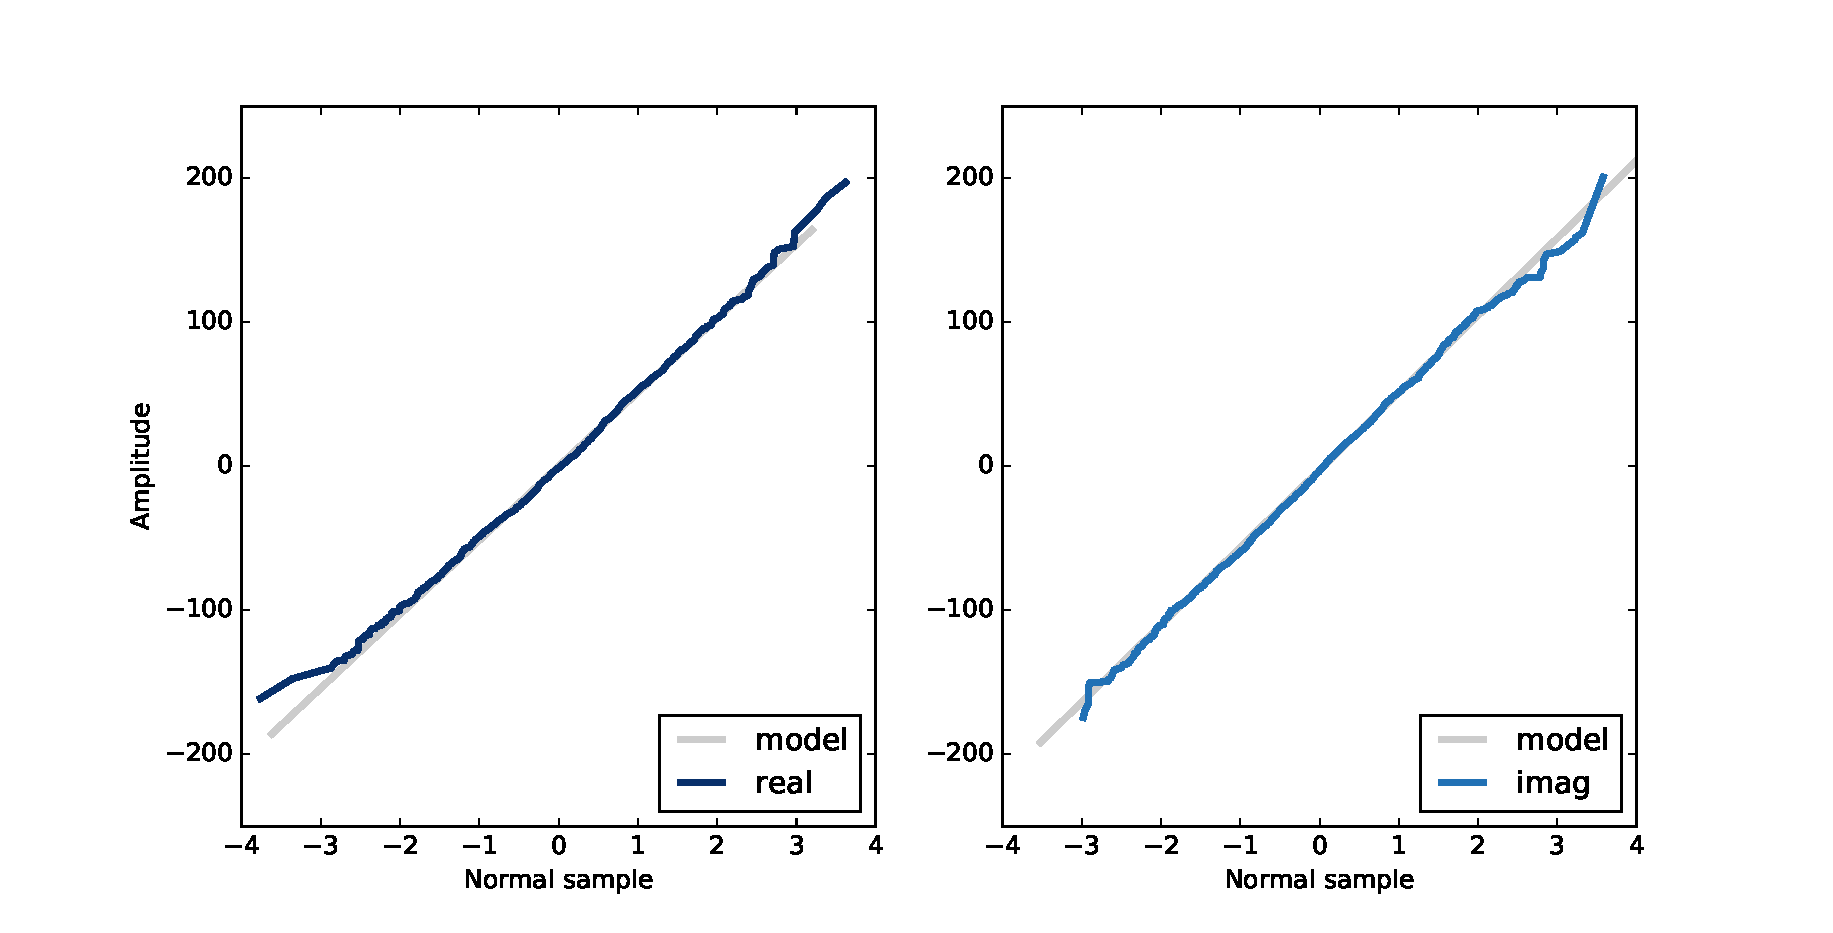
\includegraphics[height=2.5in]{figs/noise1.eps}}
\caption{Normal probability plot for the real and imaginary parts
of the spectrum of Gaussian noise.}
\label{fig.noise1}
\end{figure}

We started with uncorrelated uniform (UU) noise and showed that,
because its spectrum has equal power at all frequencies, on
average, UU noise is white.

But when people talk about ``white noise'', they don't always
mean UU noise.  In fact, more often they mean uncorrelated
Gaussian (UG) noise.

{\tt thinkdsp} provides an implementation of UG noise:

\begin{verbatim}
class UncorrelatedGaussianNoise(_Noise):

    def evaluate(self, ts):
        ys = np.random.normal(0, self.amp, len(ts))
        return ys
\end{verbatim}

{\tt np.random.normal} returns a NumPy array of values from a
Gaussian distribution, in this case with mean 0 and standard deviation
{\tt self.amp}.  In theory the range of values is from negative to
positive infinity, but we expect about 99\% of the values to be
between -3 and 3.

UG noise is similar in many ways to UU noise.  The spectrum has
equal power at all frequencies, on average, so UG is also white.
And it has one other interesting property: the spectrum of UG
noise is also UG noise.  More precisely, the real and imaginary
parts of the spectrum are uncorrelated Gaussian values.

To test that claim, we can generate the spectrum of UG noise and
then generate a ``normal probability plot'', which is a graphical
way to test whether a distribution is Gaussian.

\begin{verbatim}
    signal = thinkdsp.UncorrelatedGaussianNoise()
    wave = signal.make_wave(duration=0.5, framerate=11025)
    spectrum = wave.make_spectrum()

    thinkstats2.NormalProbabilityPlot(spectrum.real)
    thinkstats2.NormalProbabilityPlot(spectrum.imag)
\end{verbatim}

{\tt NormalProbabilityPlot} is provided by {\tt thinkstats2}, which is
included in the repository for this book.  If you are not familiar
with normal probability plots, you can read about them in Chapter 5
of {\it Think Stats} at \url{http://thinkstats2.com}.

Figure~\ref{fig.noise1} shows the results.  The gray lines
show a linear model fit to the data; the dark lines show the
data.

A straight line on a normal probability plot indicates
that the data come from a Gaussian distribution.  Except for
some random variation at the extremes, these lines are straight,
which indicates that the spectrum of UG noise is UG noise.

The spectrum of UU noise is also UG noise, at least approximately.  In
fact, by the Central Limit Theorem, the spectrum of almost any
uncorrelated noise is approximately Gaussian, as long as the
distribution has finite mean and standard deviation, and the number of
samples is large.


\section{Exercises}

Solutions to these exercises are in {\tt chap04soln.ipynb}.

\begin{exercise}
``A Soft Murmur'' is a web site that plays a mixture of natural
noise sources, including rain, waves, wind, etc.  At
\url{http://asoftmurmur.com/about/} you can find their list
of recordings, most of which are at \url{http://freesound.org}.

Download a few of these files and compute the spectrum of each
signal.  Does the power spectrum look like white noise, pink noise,
or Brownian noise?  How does the spectrum vary over time?
\end{exercise}


\begin{exercise}
In a noise signal, the mixture of frequencies changes over time.
In the long run, we expect the power at all frequencies to be equal,
but in any sample, the power at each frequency is random.

To estimate the long-term average power at each frequency, we can
break a long signal into segments, compute the power spectrum
for each segment, and then compute the average across
the segments.  You can read more about this algorithm at
\url{http://en.wikipedia.org/wiki/Bartlett's_method}.

Implement Bartlett's method and use it to estimate the power
spectrum for a noise wave.  Hint: look at the implementation
of \verb"make_spectrogram".
\end{exercise}


\begin{exercise}
At \url{http://www.coindesk.com} you can download the daily
price of a BitCoin as a CSV file.  Read this file and compute
the spectrum of BitCoin prices as a function of time.
Does it resemble white, pink, or Brownian noise?
\end{exercise}


\begin{exercise}
A Geiger counter is a device that detects radiation.
When an ionizing particle strikes the detector, it outputs a surge of
current.  The total output at a point in time can be modeled as 
uncorrelated Poisson (UP) noise, where each sample is
a random quantity from a Poisson distribution, which corresponds to the
number of particles detected during an interval.

Write a class called {\tt UncorrelatedPoissonNoise} that inherits
from \verb"thinkdsp._Noise" and provides {\tt evaluate}.  It should
use {\tt np.random.poisson} to generate random values from a Poisson
distribution.  The parameter of this function, {\tt lam}, is the
average number of particles during each interval.  You can use the
attribute {\tt amp} to specify {\tt lam}.  For example, if the
framerate is 10 kHz and {\tt amp} is 0.001, we expect about 10
``clicks'' per second.

Generate about a second of UP noise and listen to it.  For low values
of {\tt amp}, like 0.001, it should sound like a Geiger counter.  For
higher values it should sound like white noise.  Compute and plot the
power spectrum to see whether it looks like white noise.
\end{exercise}


\begin{exercise}
The algorithm in this chapter for generating pink noise is
conceptually simple but computationally expensive.  There are
more efficient alternatives, like the Voss-McCartney algorithm.
Research this method, implement it, compute the spectrum of
the result, and confirm that it has the desired relationship
between power and frequency.
\end{exercise}


\chapter{Autocorrelation}

In the previous chapter I characterized white noise as ``uncorrelated'',
which means that each value is independent of the others, and Brownian
noise as ``correlated'', because each value depends on the preceding
value.  In this chapter I define these terms more precisely and
present the {\bf autocorrelation function}, which is a useful tool
for signal analysis.

The code for this chapter is in {\tt chap05.ipynb}, which is in the
repository for this book (see Section~\ref{code}).
You can also view it at \url{http://tinyurl.com/thinkdsp05}.


\section{Correlation}

In general, correlation between variables means that if you know the
value of one, you have some information about the other.  There are
several ways to quantify correlation, but the most common is the
Pearson product-moment correlation coefficient, usually denoted
$\rho$.  For two variables, $x$ and $y$, that each contain $N$ values:
%
\[ \rho = \frac{ \sum_i (x_i - \mu_x) (y_i - \mu_y)}{N \sigma_x \sigma_y} \]
%
Where $\mu_x$ and $\mu_y$ are the means of $x$ and $y$, and
$\sigma_x$ and $\sigma_y$ are their standard deviations.

Pearson's correlation is always between -1 and +1 (including both).
If $\rho$ is positive, we say that the correlation is positive,
which means that when one variable is high, the other tends to be
high.  If $\rho$ is negative, the correlation is negative, so
when one variable is high, the other tends to be low.

The magnitude of $\rho$ indicates the strength of the correlation.  If
$\rho$ is 1 or -1, the variables are perfectly correlated, which means
that if you know one, you can make a perfect prediction about the
other.  If $\rho$ is near zero, the correlation is probably weak, so
if you know one, it doesn't tell you much about the others,

I say ``probably weak'' because it is also possible that there is
a nonlinear relationship that is not captured by the coefficient
of correlation.  Nonlinear relationships are often important in
statistics, but less often relevant for signal processing, so I
won't say more about them here.

Python provides several ways to compute correlations.  {\tt
  np.corrcoef} takes any number of variables and computes a {\bf
  correlation matrix} that includes correlations between each pair of
variables.

\begin{figure}
% autocorr.py
\centerline{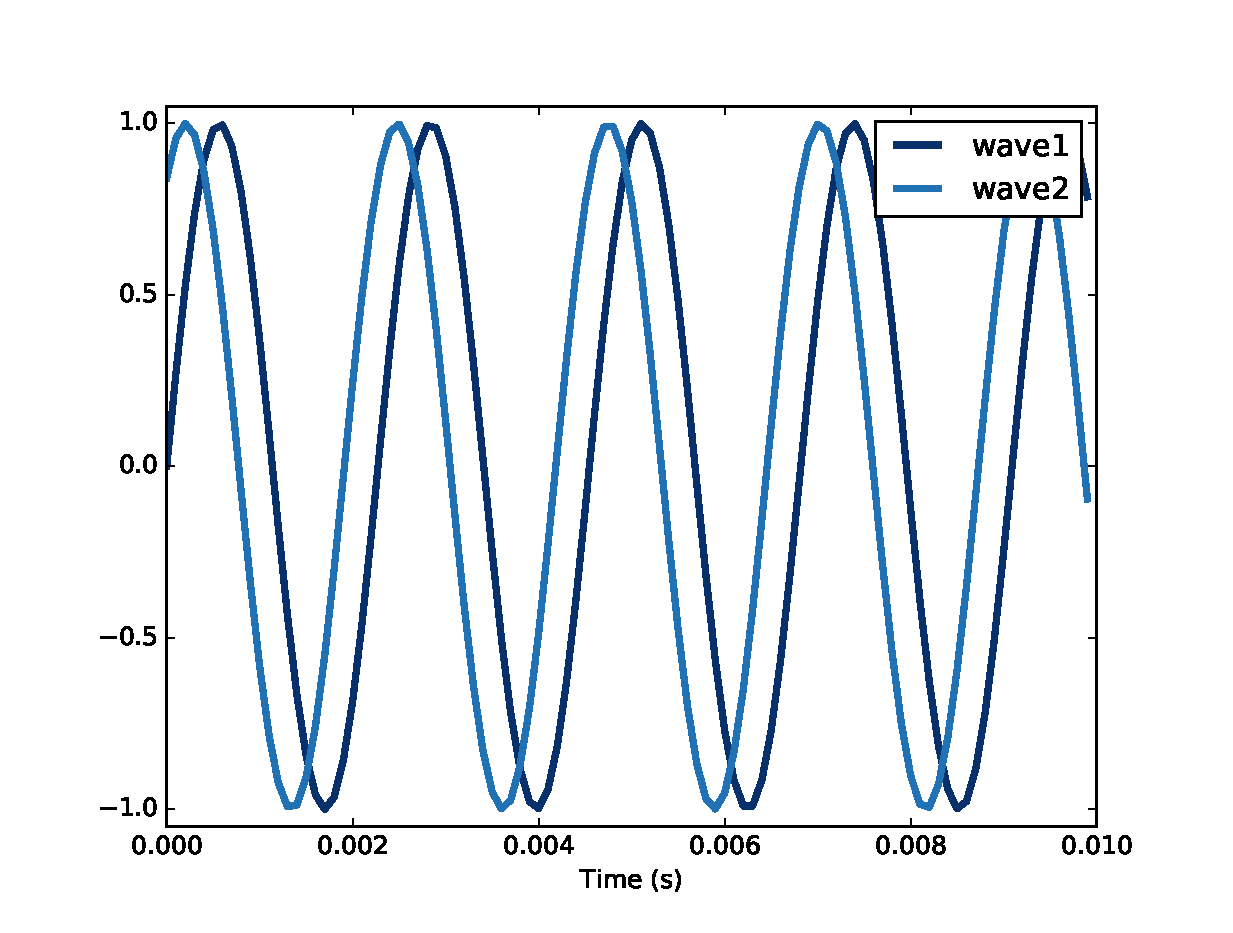
\includegraphics[height=2.5in]{figs/autocorr1.eps}}
\caption{Two sine waves that differ by a phase offset of 1 radian;
their coefficient of correlation is 0.54.}
\label{fig.autocorr1}
\end{figure}

I'll present an example with only two variables.  First, I define
a function that constructs sine waves with different phase offsets:

\begin{verbatim}
def make_sine(offset):
    signal = thinkdsp.SinSignal(freq=440, offset=offset)
    wave = signal.make_wave(duration=0.5, framerate=10000)
    return wave
\end{verbatim}

Next I instantiate two waves with different offsets:

\begin{verbatim}
wave1 = make_sine(offset=0)
wave2 = make_sine(offset=1)
\end{verbatim}

Figure~\ref{fig.autocorr1} shows what the first few periods of these
waves look like.  When one wave is high, the other is usually high, so we
expect them to be correlated.

\begin{verbatim}
>>> corr_matrix = np.corrcoef(wave1.ys, wave2.ys, ddof=0)
[[ 1.    0.54]
 [ 0.54  1.  ]]
\end{verbatim}

The option {\tt ddof=0} indicates that {\tt corrcoef} should divide by
$N$, as in the equation above, rather than use the default, $N-1$.

The result is a correlation matrix:
the first element is the correlation of {\tt wave1}
with itself, which is always 1.  Similarly, the last element
is the correlation of {\tt wave2} with itself.

\begin{figure}
% autocorr.py
\centerline{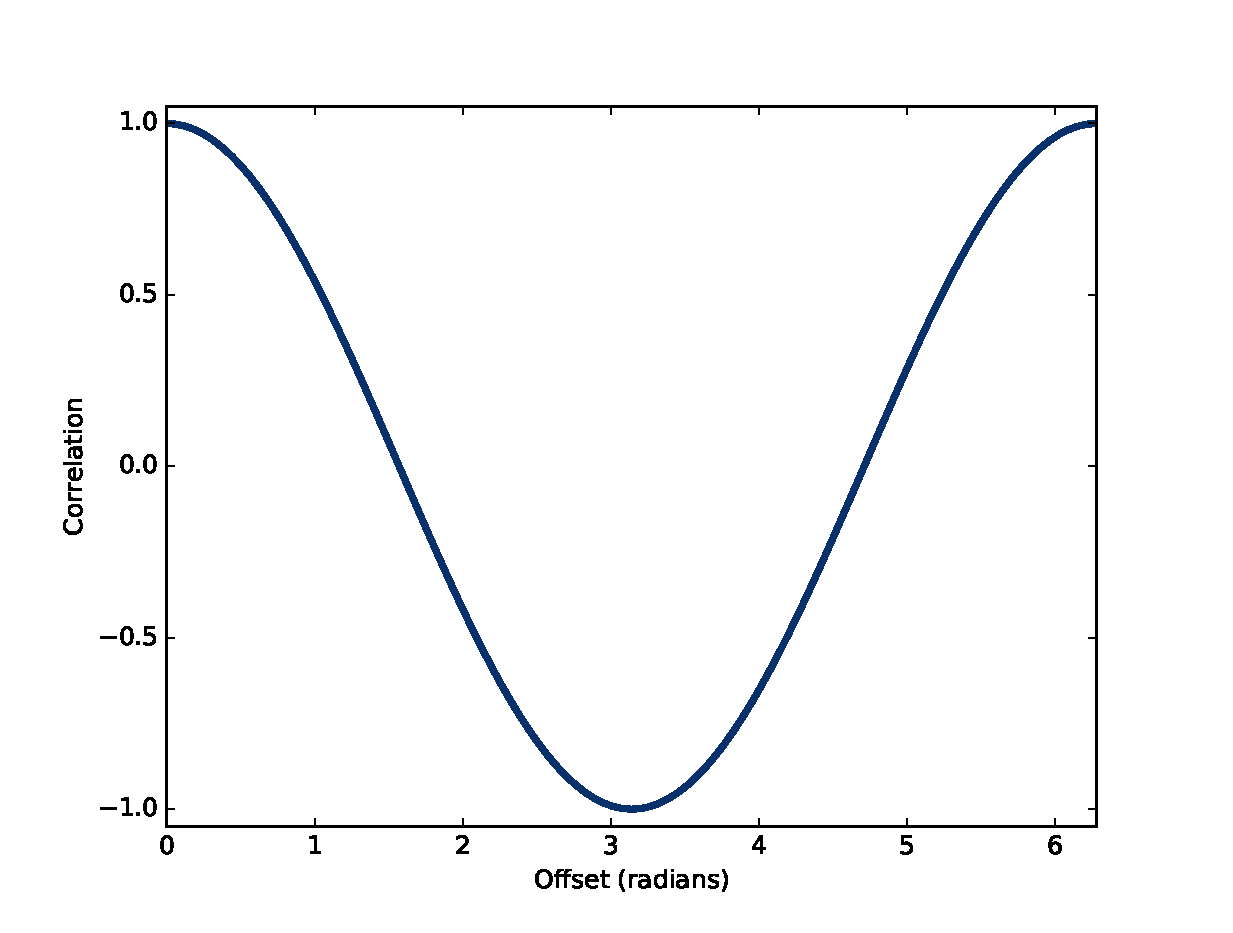
\includegraphics[height=2.5in]{figs/autocorr2.eps}}
\caption{The correlation of two sine waves as a function of the
phase offset between them.  The result is a cosine.}
\label{fig.autocorr2}
\end{figure}

The off-diagonal elements contain the value we're interested in,
the correlation of {\tt wave1} and {\tt wave2}.  The value 0.54
indicates that the strength of the correlation is moderate.

As the phase offset increases, this correlation decreases until
the waves are 180 degrees out of phase, which yields correlation
-1.  Then it increases until the offset differs by 360 degrees.
At that point we have come full circle and the correlation is 1.

Figure~\ref{fig.autocorr2} shows the relationship between correlation and
phase offset for a sine wave.  The shape of that curve should look
familiar; it is a cosine.  

{\tt thinkdsp} provides a simple interface for computing the
correlation between waves:

\begin{verbatim}
>>> wave1.corr(wave2)
0.54
\end{verbatim}


\section{Serial correlation}

Signals often represent measurements of quantities that vary in
time.  For example, the sound signals we've worked with represent
measurements of voltage (or current), which correspond to the changes
in air pressure we perceive as sound.

Measurements like this almost always have serial correlation, which
is the correlation between each element and the next (or the previous).
To compute serial correlation, we can shift a signal and then compute
the correlation of the shifted version with the original.

\begin{verbatim}
def serial_corr(wave, lag=1):
    n = len(wave)
    y1 = wave.ys[lag:]
    y2 = wave.ys[:n-lag]
    corr = np.corrcoef(y1, y2, ddof=0)[0, 1]
    return corr
\end{verbatim}

\verb"serial_corr" takes a Wave object and
{\tt lag}, which is the integer number of places to shift the wave.
It computes the correlation of the wave with a shifted version
of itself.

We can test this function with the noise signals from the previous
chapter.  We expect UU noise to be uncorrelated, based on the
way it's generated (not to mention the name):

\begin{verbatim}
signal = thinkdsp.UncorrelatedGaussianNoise()
wave = signal.make_wave(duration=0.5, framerate=11025)
serial_corr(wave)
\end{verbatim}

When I ran this example, I got 0.006, which indicates a very
small serial correlation.  You might get a different value when you run
it, but it should be comparably small.

In a Brownian noise signal, each value is the sum of the previous
value and a random ``step'', so we expect a strong serial
correlation:

\begin{verbatim}
signal = thinkdsp.BrownianNoise()
wave = signal.make_wave(duration=0.5, framerate=11025)
serial_corr(wave)
\end{verbatim}

Sure enough, the result I got is greater than 0.999.

\begin{figure}
% autocorr.py
\centerline{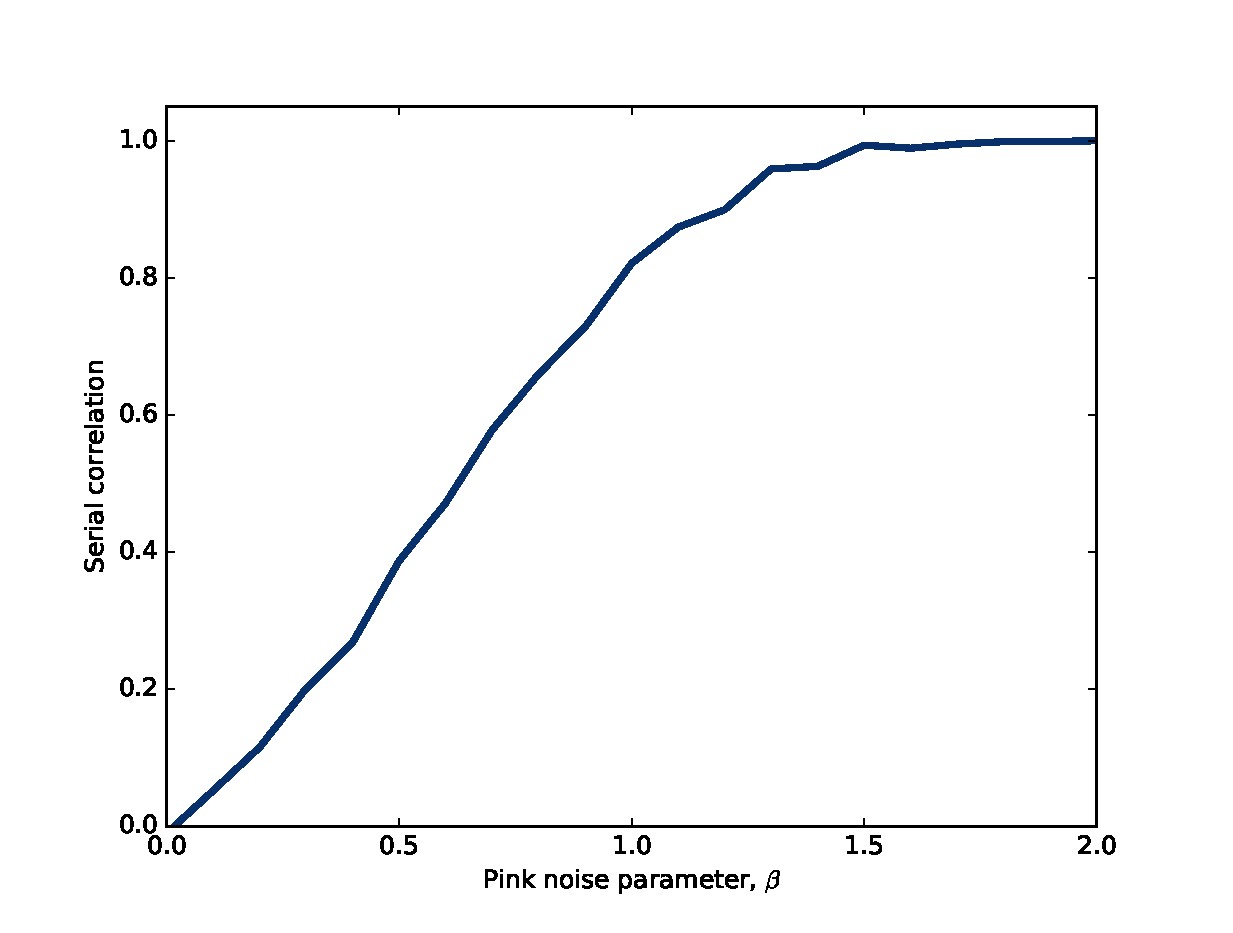
\includegraphics[height=2.5in]{figs/autocorr3.eps}}
\caption{Serial correlation for pink noise with a range of
parameters.}
\label{fig.autocorr3}
\end{figure}

Since pink noise is in some sense between Brownian noise and UU noise,
we might expect an intermediate correlation:

\begin{verbatim}
signal = thinkdsp.PinkNoise(beta=1)
wave = signal.make_wave(duration=0.5, framerate=11025)
serial_corr(wave)
\end{verbatim}

With parameter $\beta=1$, I got a serial correlation of 0.851.
As we vary the parameter from $\beta=0$, which is uncorrelated
noise, to $\beta=2$, which is Brownian, serial correlation
ranges from 0 to almost 1, as shown in Figure~\ref{fig.autocorr3}.


\section{Autocorrelation}
\label{autopink}

In the previous section we computed the correlation between each
value and the next, so we shifted the elements of the array by 1.
But we can easily compute serial correlations with
different lags.

\begin{figure}
% autocorr.py
\centerline{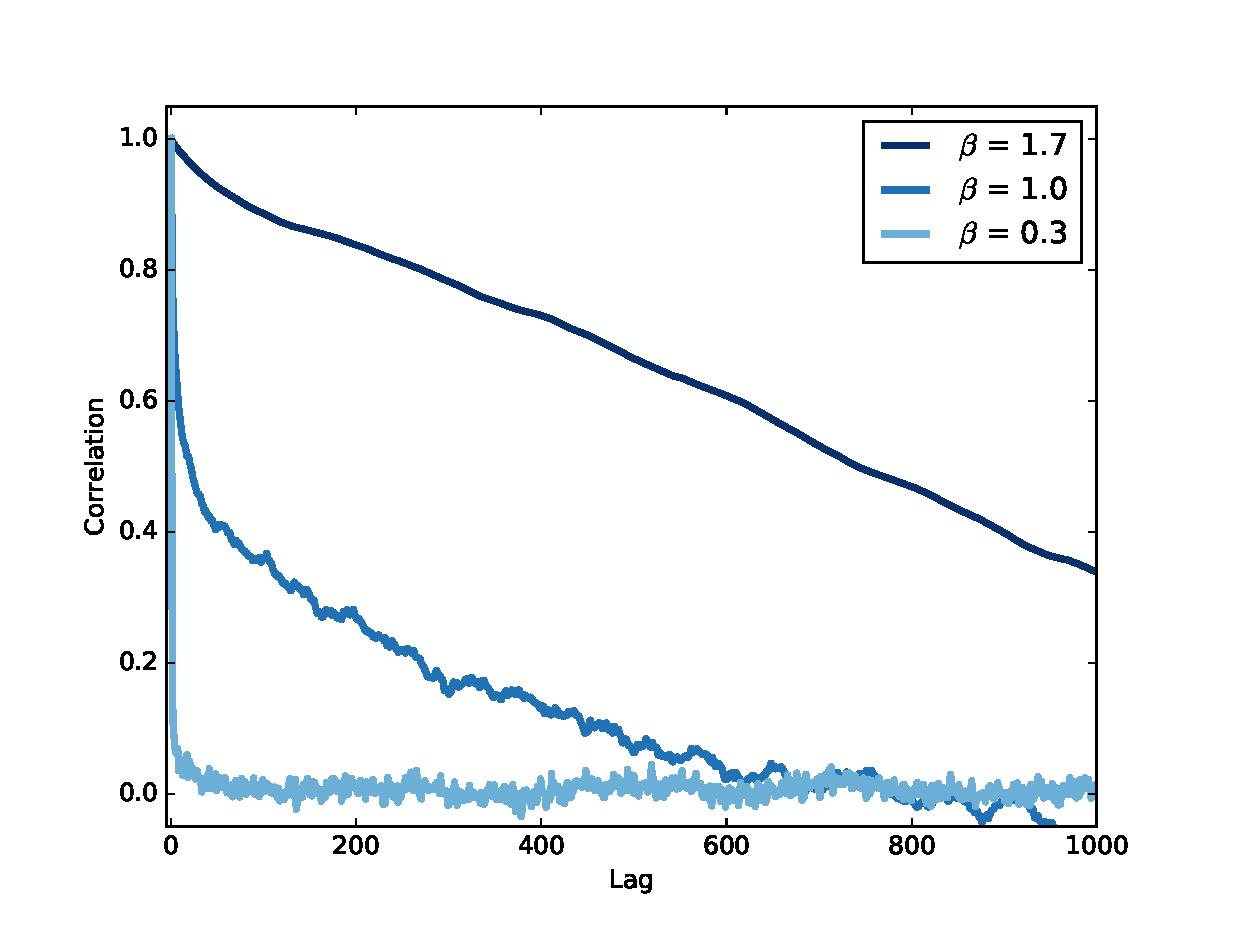
\includegraphics[height=2.5in]{figs/autocorr4.eps}}
\caption{Autocorrelation functions for pink noise with a range
of parameters.}
\label{fig.autocorr4}
\end{figure}

You can think of \verb"serial_corr" as a function that
maps from each value of lag to the corresponding correlation, and we
can evaluate that function by looping through values of {\tt lag}:

\begin{verbatim}
def autocorr(wave):
    lags = range(len(wave.ys)//2)
    corrs = [serial_corr(wave, lag) for lag in lags]
    return lags, corrs
\end{verbatim}

{\tt autocorr} takes a Wave object and returns the autocorrelation
function as a pair of sequences: {\tt lags} is a sequence of
integers from 0 to half the length of the wave; {\tt corrs}
is the sequence of serial correlations for each lag.

Figure~\ref{fig.autocorr4} shows autocorrelation functions for pink
noise with three values of $\beta$.  For low values of $\beta$, the
signal is less correlated, and the autocorrelation function drops
off to zero quickly.  For larger values, serial correlation
is stronger and drops off more slowly.  With $\beta=1.7$ serial
correlation is strong even for long lags; this phenomenon is called
{\bf long-range dependence}, because it indicates that each value in
the signal depends on many preceding values.


\section{Autocorrelation of periodic signals}

The autocorrelation of pink noise has interesting mathematical
properties, but limited applications.  The autocorrelation of
periodic signals is more useful.

\begin{figure}
% autocorr.py
\centerline{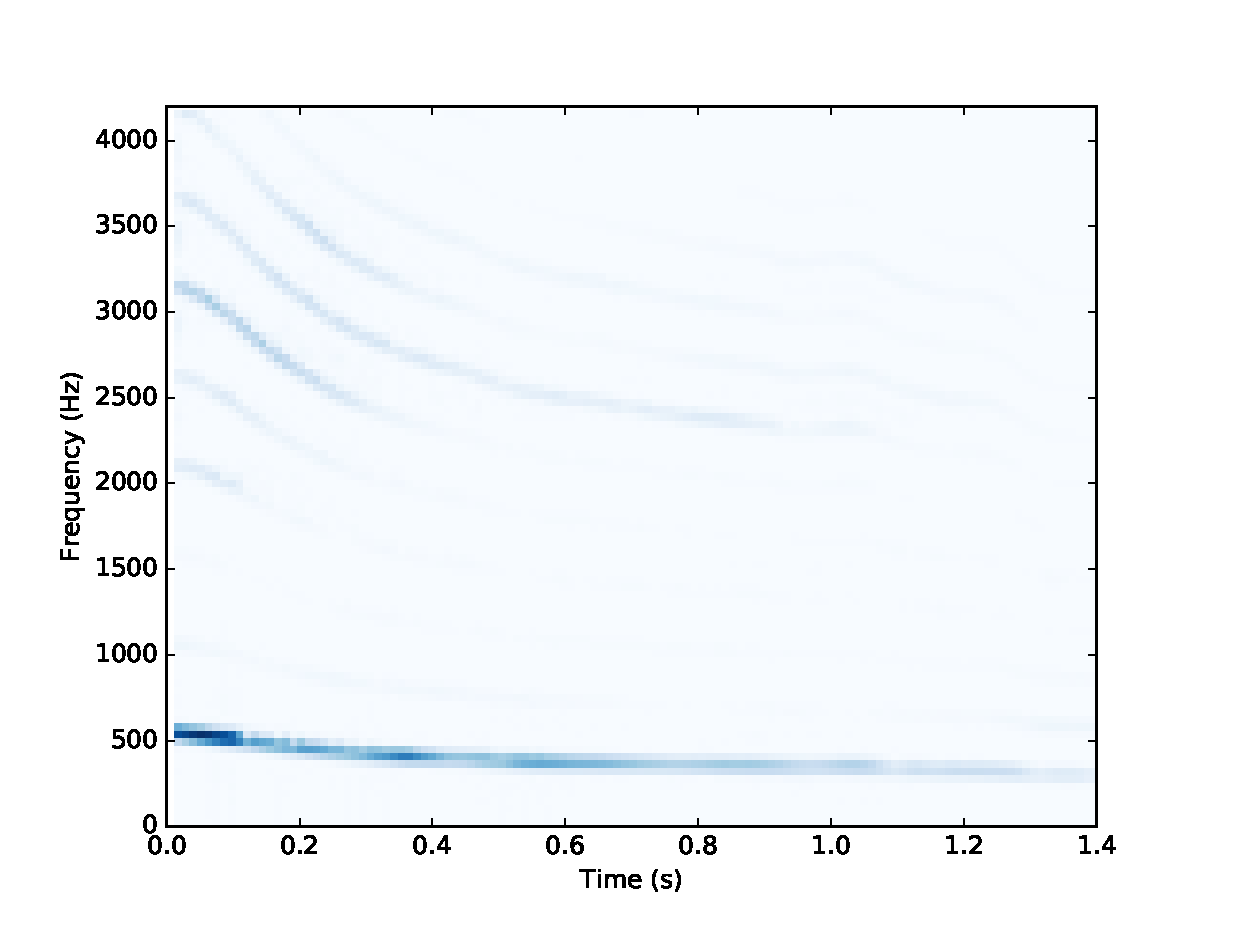
\includegraphics[height=2.5in]{figs/autocorr5.eps}}
\caption{Spectrogram of a vocal chirp.}
\label{fig.autocorr5}
\end{figure}

As an example, I downloaded from \url{freesound.org} a recording of
someone singing a chirp; the repository for this book includes the
file: \url{28042__bcjordan__voicedownbew.wav}.  You can use the
IPython notebook for this chapter, {\tt chap05.ipynb}, to play it.

Figure~\ref{fig.autocorr5} shows the spectrogram of this wave.
The fundamental frequency and some of the harmonics show up clearly.
The chirp starts near 500 Hz and drops down to about 300 Hz, roughly
from C5 to E4.

\begin{figure}
% autocorr.py
\centerline{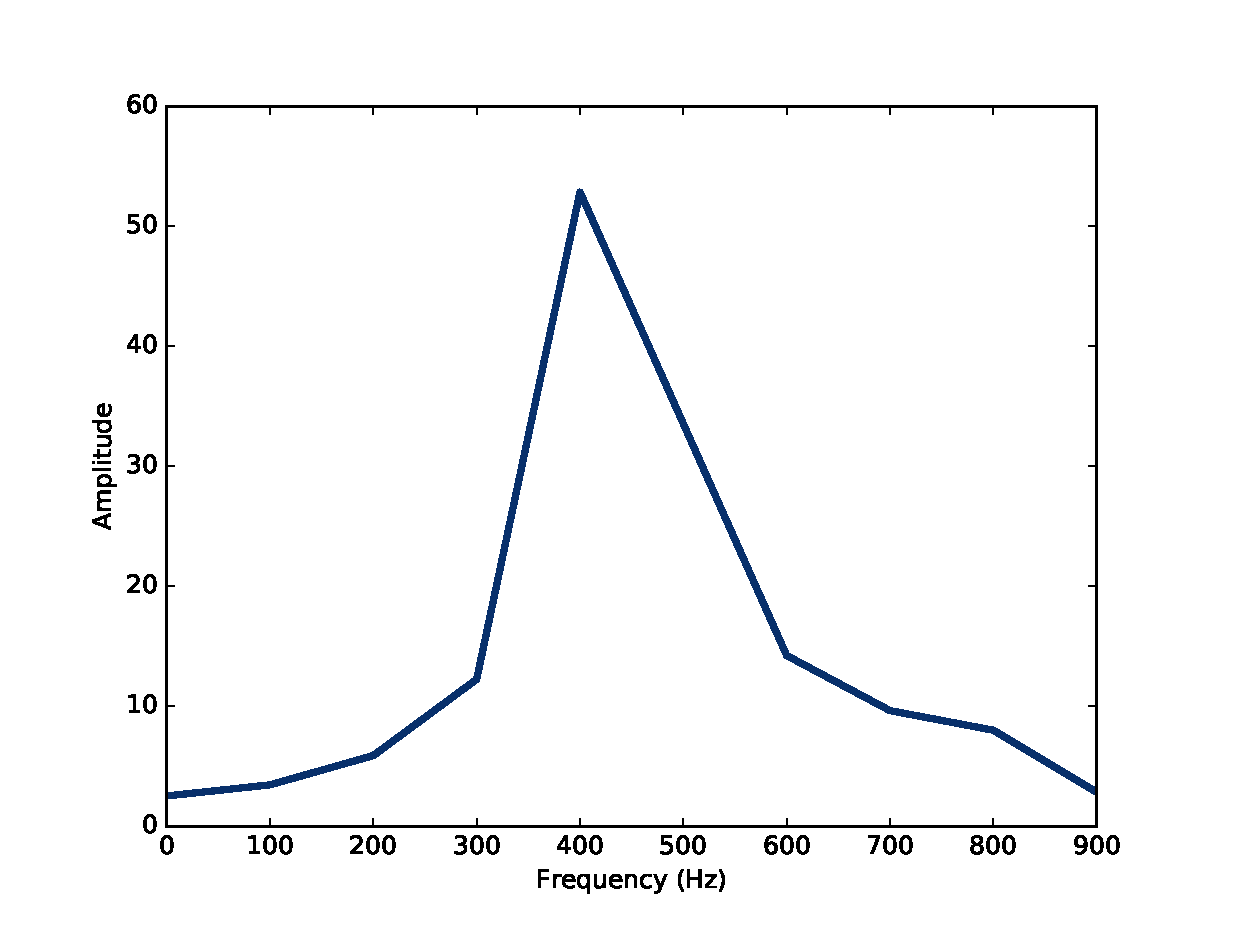
\includegraphics[height=2.5in]{figs/autocorr6.eps}}
\caption{Spectrum of a segment from a vocal chirp.}
\label{fig.autocorr6}
\end{figure}

To estimate pitch at a particular point in time, we could use the
spectrum, but it doesn't work very well.  To see why not, I'll take
a short segment from the wave and plot its spectrum:

\begin{verbatim}
    duration = 0.01
    segment = wave.segment(start=0.2, duration=duration)
    spectrum = segment.make_spectrum()
    spectrum.plot(high=1000)
\end{verbatim}

This segment starts at 0.2 seconds and lasts 0.01 seconds.
Figure~\ref{fig.autocorr6} shows its spectrum.  There is a clear peak
near 400 Hz, but it is hard to identify the pitch precisely.  The
length of the segment is 441 samples at a framerate of 44100 Hz, so
the frequency resolution is 100 Hz (see Section~\ref{gabor}).
That means the estimated pitch might be off by 50 Hz; in musical
terms, the range from 350 Hz to 450 Hz is about 5 semitones, which is
a big difference!

We could get better frequency resolution by taking a longer segment,
but since the pitch is changing over time, we would also get ``motion
blur''; that is, the peak would spread between the start and end pitch of
the segment, as we saw in Section~\ref{sauron}.

We can estimate pitch more precisely using autocorrelation.
If a signal is periodic, we expect the autocorrelation to spike
when the lag equals the period.

\begin{figure}
% autocorr.py
\centerline{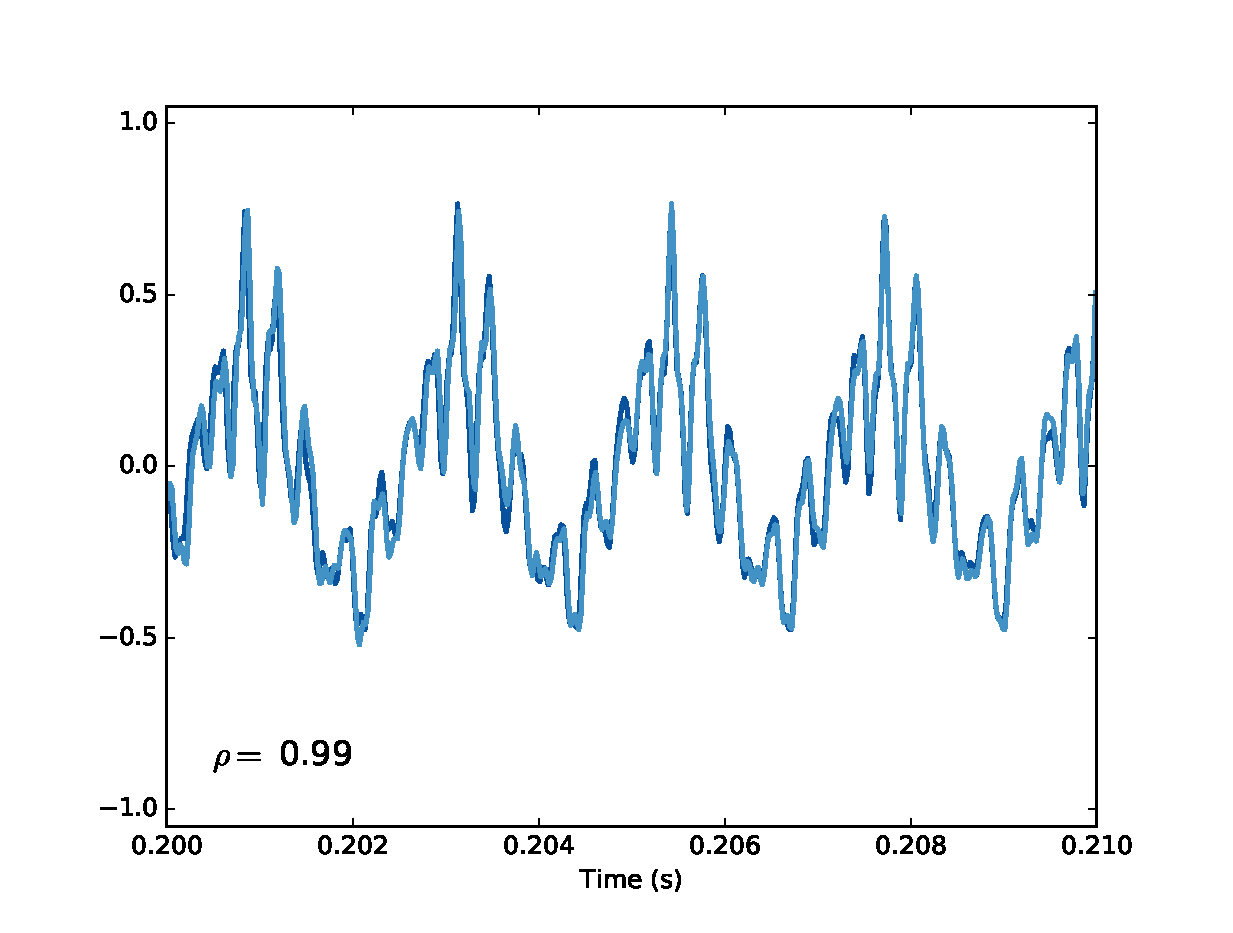
\includegraphics[height=2.5in]{figs/autocorr7.eps}}
\caption{Two segments from a chirp, one starting 0.0023 seconds
after the other.}
\label{fig.autocorr7}
\end{figure}

To show why that works, I'll plot two segments from the same
recording.

\begin{verbatim}
def plot_shifted(wave, offset=0.001, start=0.2):
    thinkplot.preplot(2)
    segment1 = wave.segment(start=start, duration=0.01)
    segment1.plot(linewidth=2, alpha=0.8)

    segment2 = wave.segment(start=start-offset, duration=0.01)
    segment2.shift(offset)
    segment2.plot(linewidth=2, alpha=0.4)

    corr = segment1.corr(segment2)
    text = r'$\rho =$ %.2g' % corr
    thinkplot.text(segment1.start+0.0005, -0.8, text)
    thinkplot.config(xlabel='Time (s)')
\end{verbatim} 

One segment starts at 0.2 seconds; the other starts 0.0023 seconds
later.  Figure~\ref{fig.autocorr7} shows the result.  The segments
are similar, and their correlation is 0.99.  This result suggests
that the period is near 0.0023 seconds, which corresponds to a frequency
of 435 Hz.

\begin{figure}
% autocorr.py
\centerline{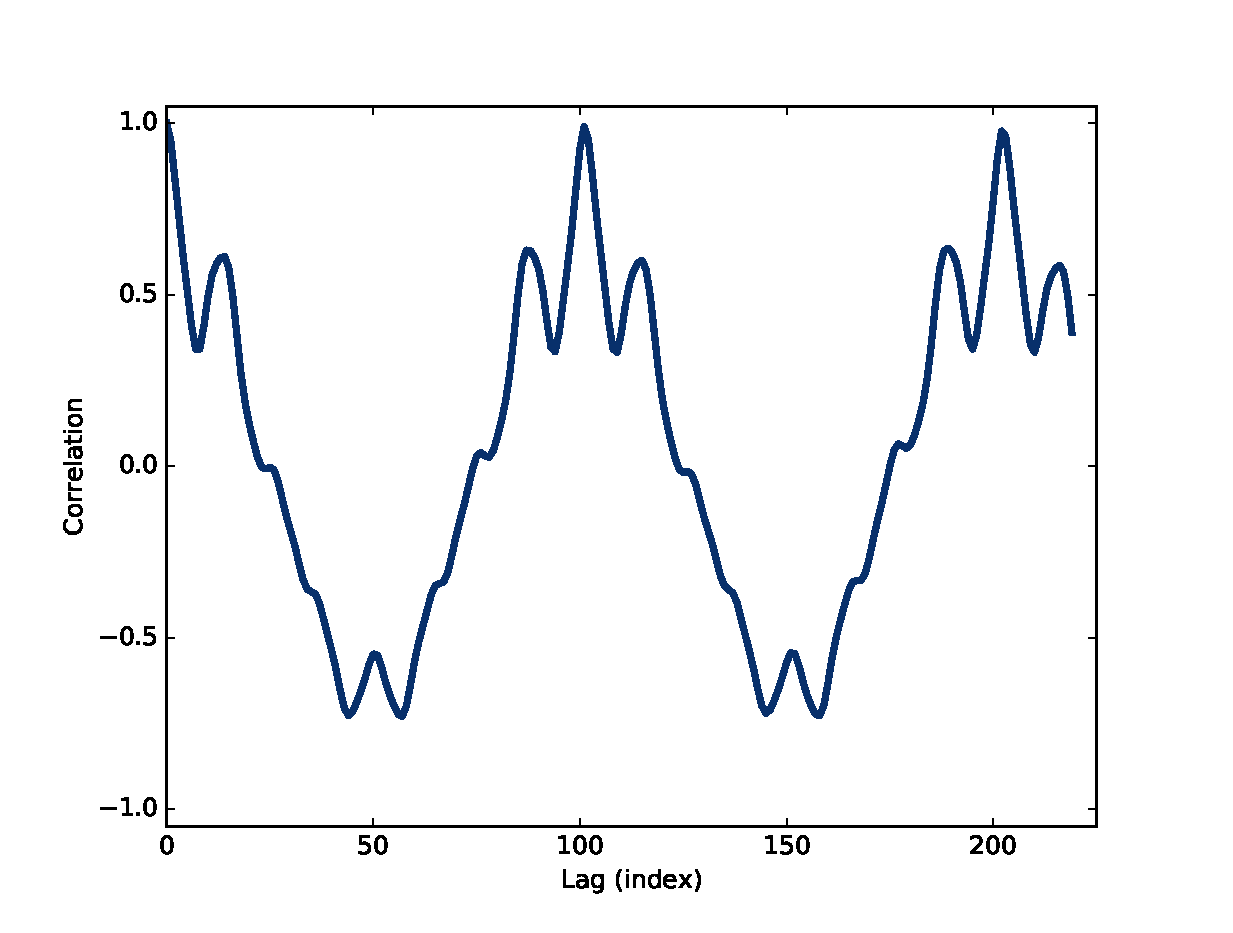
\includegraphics[height=2.5in]{figs/autocorr8.eps}}
\caption{Autocorrelation function for a segment from a chirp.}
\label{fig.autocorr8}
\end{figure}

For this example, I estimated the period by trial and error.  To automate
the process, we can use the autocorrelation function.

\begin{verbatim}
    lags, corrs = autocorr(segment)
    thinkplot.plot(lags, corrs)
\end{verbatim}

Figure~\ref{fig.autocorr8} shows the autocorrelation function for
the segment starting at $t=0.2$ seconds.  The first peak occurs at
{\tt lag=101}.  We can compute the frequency that corresponds
to that period like this:

\begin{verbatim}
    period = lag / segment.framerate
    frequency = 1 / period
\end{verbatim}

The estimated fundamental frequency is 437 Hz.  To evaluate the
precision of the estimate, we can run the same computation with
lags 100 and 102, which correspond to frequencies 432 and 441 Hz.
The frequency precision using autocorrelation is less than 10 Hz,
compared with 100 Hz using the spectrum.  In musical terms, the
expected error is about 30 cents (a third of a semitone).


\section{Correlation as dot product}
\label{dotproduct}

I started the chapter with this definition of Pearson's
correlation coefficient:
%
\[ \rho = \frac{ \sum_i (x_i - \mu_x) (y_i - \mu_y)}{N \sigma_x \sigma_y} \]
%
Then I used $\rho$ to define serial correlation and autocorrelation.
That's consistent with how these terms are used in statistics,
but in the context of signal processing, the definitions are
a little different.

In signal processing, we are often working with unbiased signals,
where the mean is 0, and normalized signals, where the standard
deviation is 1.  In that case, the definition of $\rho$ simplifies to:
%
\[ \rho = \frac{1}{N} \sum_i x_i y_i \]
%
And it is common to simplify even further:
%
\[ r = \sum_i x_i y_i \]
%
This definition of correlation is not ``standardized'', so it doesn't
generally fall between -1 and 1.  But it has other useful properties.

If you think of $x$ and $y$ as vectors, you might recognize this
formula as the {\bf dot product}, $x \cdot y$.  See
\url{http://en.wikipedia.org/wiki/Dot_product}.

\newcommand{\norm}{\mathrm{norm}}

The dot product indicates the degree to which the signals are similar.
If they are normalized so their standard deviations are 1,
%
\[ x \cdot y = \cos \theta \]
%
where $\theta$ is the angle between the vectors.  And that explains
why Figure~\ref{fig.autocorr2} is a cosine curve.


\section{Using NumPy}
\label{correlate}

\begin{figure}
% autocorr.py
\centerline{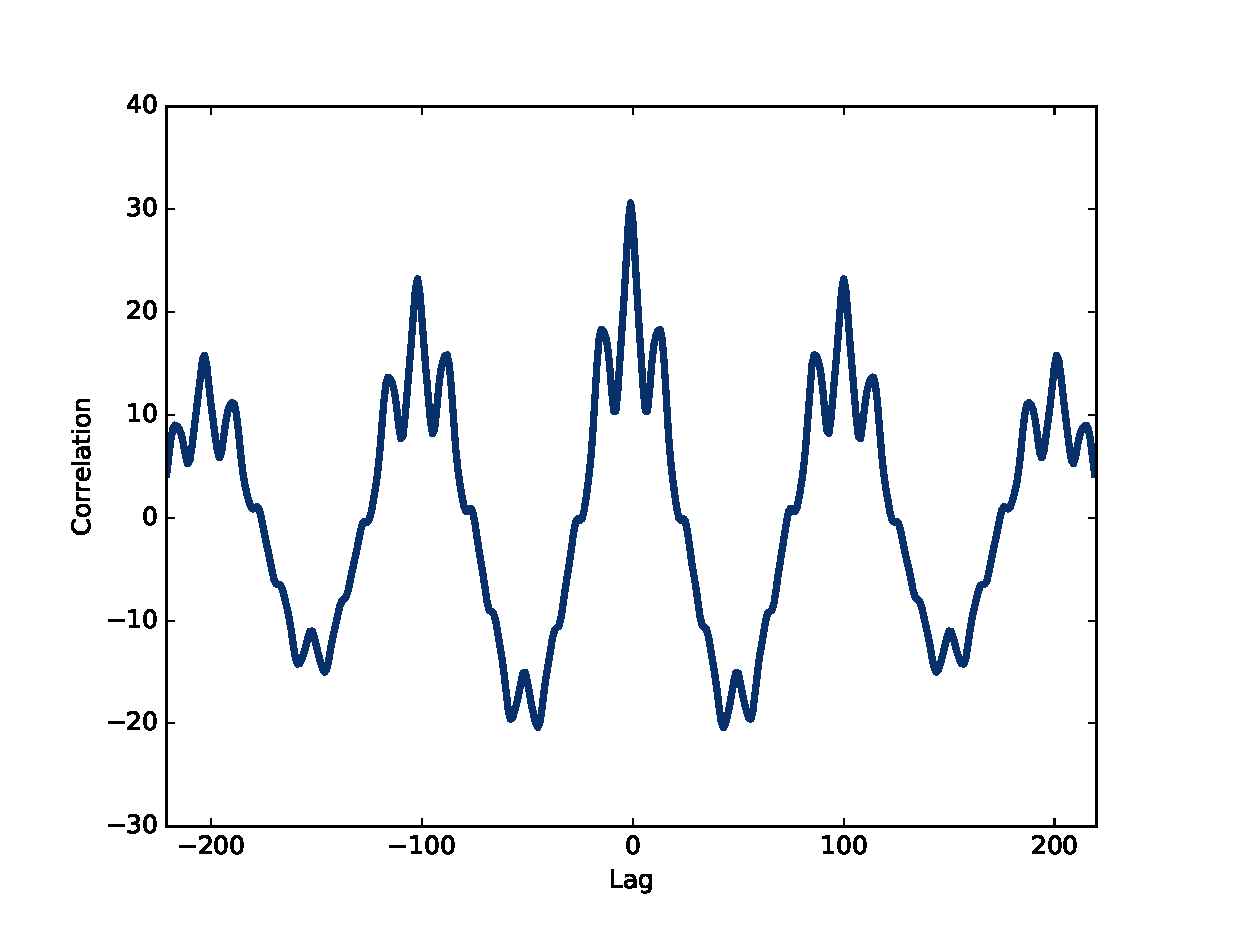
\includegraphics[height=2.5in]{figs/autocorr9.eps}}
\caption{Autocorrelation function computed with {\tt np.correlate}.}
\label{fig.autocorr9}
\end{figure}

NumPy provides a function, {\tt correlate}, that computes
the correlation of two functions or the autocorrelation of one
function.  We can use it to compute the autocorrelation of
the segment from the previous section:

\begin{verbatim}
corrs2 = np.correlate(segment.ys, segment.ys, mode='same')
\end{verbatim}

The option {\tt mode} tells {\tt correlate} what range
of {\tt lag} to use.  With the value {\tt 'same'}, the
range is from $-N/2$ to $N/2$, where $N$ is the length of the
wave array.

Figure~\ref{fig.autocorr9} shows the result.  It is symmetric because
the two signals are identical, so a negative lag on one has the same
effect as a positive lag on the other.  To compare with the results
from {\tt autocorr}, we can select the second half:

\begin{verbatim}
    N = len(corrs2)
    half = corrs2[N//2:]
\end{verbatim}

If you compare Figure~\ref{fig.autocorr9} to Figure~\ref{fig.autocorr8},
you'll notice that the correlations computed by {\tt np.correlate}
get smaller as the lags increase.  That's because {\tt np.correlate}
uses the unstandardized definition of correlation;
as the lag gets bigger, the
overlap between the two signals gets smaller, so the magnitude of
the correlations decreases.

We can correct that by dividing through by the lengths:

\begin{verbatim}
    lengths = range(N, N//2, -1)
    half /= lengths
\end{verbatim}

Finally, we can standardize the results so the correlation with
{\tt lag=0} is 1.

\begin{verbatim}
    half /= half[0]
\end{verbatim}

With these adjustments, the results computed by {\tt autocorr} and
{\tt np.correlate} are nearly the same.  They still differ by
1-2\%.  The reason is not important, but if you are curious: {\tt autocorr}
standardizes the correlations independently for each lag; for
{\tt np.correlate}, we standardized them all at the end.

More importantly, now you know what autocorrelation is, how to
use it to estimate the fundamental period of a signal, and two
ways to compute it.


\section{Exercises}

Solutions to these exercises are in {\tt chap05soln.ipynb}.

\begin{exercise}
The IPython notebook for this chapter, {\tt chap05.ipynb}, includes
an interaction that lets you compute autocorrelations for different
lags.  Use this interaction to estimate the pitch of the vocal chirp
for a few different start times.
\end{exercise}


\begin{exercise}
The example code in \verb"chap05.ipynb" shows how to use autocorrelation
to estimate the fundamental frequency of a periodic signal.
Encapsulate this code in a function called \verb"estimate_fundamental",
and use it to track the pitch of a recorded sound.

To see how well it works, try superimposing your pitch estimates on a
spectrogram of the recording.
\end{exercise}


\begin{exercise}
If you did the exercises in the previous chapter, you downloaded
the historical price of BitCoins and estimated the power spectrum
of the price changes.  Using the same data, compute the autocorrelation
of BitCoin prices.  Does the autocorrelation function drop off quickly?
Is there evidence of periodic behavior?
\end{exercise}


\begin{exercise}
In the repository for this book you will find an IPython notebook
called \verb"saxophone.ipynb" that explores autocorrelation,
pitch perception, and a phenomenon called the ``missing fundamental''.
Read through this notebook and run the examples.  Try selecting
a different segment of the recording and running the examples again.
\end{exercise}



\chapter{Discrete cosine transform}
\label{dct}

The topic of this chapter is the {\bf Discrete Cosine
  Transform} (DCT), which is used in MP3 and related formats for
compressing music; JPEG and similar formats for images; and the MPEG
family of formats for video.

DCT is similar in many ways to the Discrete Fourier Transform (DFT),
which we have been using for spectral analysis.
Once we learn how DCT works, it will be easier to explain DFT.

Here are the steps to get there:

\begin{enumerate}

\item We'll start with the synthesis problem: given a set of frequency
  components and their amplitudes, how can we construct a wave?

\item Next we'll rewrite the synthesis problem using NumPy arrays.
  This move is good for performance, and also provides insight
  for the next step.

\item We'll look at the analysis problem: given a signal and a
  set of frequencies, how can we find the amplitude of each frequency
  component?  We'll start with a solution that is conceptually simple
  but slow.

\item Finally, we'll use some principles from linear algebra to find a
  more efficient algorithm.  If you already know linear algebra,
  that's great, but I'll explain what you need as we go.

\end{enumerate}

The code for this chapter is in {\tt
  chap06.ipynb} which is in the repository for this book (see
Section~\ref{code}).
You can also view it at \url{http://tinyurl.com/thinkdsp06}.


\section{Synthesis}
\label{synth1}

Suppose I give you a list of amplitudes and a list of frequencies,
and ask you to construct a signal that is the sum of these frequency
components.  Using objects in the {\tt thinkdsp} module, there is
a simple way to perform this operation, which is called {\bf synthesis}:

\begin{verbatim}
def synthesize1(amps, fs, ts):
    components = [thinkdsp.CosSignal(freq, amp)
                  for amp, freq in zip(amps, fs)]
    signal = thinkdsp.SumSignal(*components)

    ys = signal.evaluate(ts)
    return ys
\end{verbatim}

{\tt amps} is a list of amplitudes, {\tt fs} is the list
of frequencies, and {\tt ts} is the sequence
of times where the signal should be evaluated.

{\tt components} is a list of {\tt CosSignal} objects, one for
each amplitude-frequency pair.  {\tt SumSignal} represents the
sum of these frequency components.

Finally, {\tt evaluate} computes the value of the signal at each
time in {\tt ts}.

We can test this function like this:

\begin{verbatim}
    amps = np.array([0.6, 0.25, 0.1, 0.05])
    fs = [100, 200, 300, 400]
    framerate = 11025

    ts = np.linspace(0, 1, framerate)
    ys = synthesize1(amps, fs, ts)
    wave = thinkdsp.Wave(ys, framerate)
\end{verbatim}

This example makes a signal that contains a fundamental frequency at
100 Hz and three harmonics (100 Hz is a sharp G2).  It renders the
signal for one second at 11,025 frames per second and puts the results
into a Wave object.

Conceptually, synthesis is pretty simple.  But in this form it doesn't
help much with {\bf analysis}, which is the inverse problem: given the
wave, how do we identify the frequency components and their amplitudes?


\section{Synthesis with arrays}
\label{synthesis}

\begin{figure}
% LaTeX source for ``Think DSP: Digital Signal Processing for Programmers''
% Copyright 2013  Allen B. Downey.

% License: Creative Commons Attribution-NonCommercial 3.0 Unported License.
% http://creativecommons.org/licenses/by-nc/3.0/
%

\[ 
\begin{matrix}
& {\large \mathtt{M}} &
 \begin{bmatrix} 
0.6 \\
0.25 \\
0.1 \\
0.05 \\
\end{bmatrix}
= \mathtt{amps}
\\
\\
\begin{matrix} 
&.& \\
&.& \\
&t_n& \\
&.& \\
&.& \\
\end{matrix}
&
\begin{bmatrix} 
. & . & . & . \\
. & . & . & . \\
a & b & c & d \\
. & . & . & . \\
. & . & . & . \\
\end{bmatrix} 
&
\begin{bmatrix} 
&.& \\
&.& \\
&e& \\
&.& \\
&.& \\
\end{bmatrix} = \mathtt{ys}
\\
\\
&
\begin{matrix}
. & f_k & . & . \\
\end{matrix}
&
\\
\end{matrix}
\]


 

\caption{Synthesis with arrays.}
\label{fig.synthesis}
\end{figure}

Here's another way to write {\tt synthesize}:

\begin{verbatim}
def synthesize2(amps, fs, ts):
    args = np.outer(ts, fs)
    M = np.cos(PI2 * args)
    ys = np.dot(M, amps)
    return ys
\end{verbatim}

This function looks very different, but it does the same thing.
Let's see how it works:

\begin{enumerate}

\item {\tt np.outer} computes the outer product of {\tt ts} and
  {\tt fs}.  The result is an array with one row for each element
  of {\tt ts} and one column for each element of {\tt fs}.  Each
  element in the array is the product of a frequency and a time, $f
  t$.

\item We multiply {\tt args} by $2 \pi$ and apply {\tt cos}, so each
  element of the result is $\cos (2 \pi f t)$.  Since the {\tt ts} run
  down the columns, each column contains a cosine signal at a
  particular frequency, evaluated at a sequence of times.

\item {\tt np.dot} multiplies each row of {\tt M} by {\tt amps},
  element-wise, and then adds up the products.  In terms of linear
  algebra, we are multiplying a matrix, {\tt M}, by a vector, {\tt
    amps}.  In terms of signals, we are computing the weighted sum
  of frequency components.

\end{enumerate}

Figure~\ref{fig.synthesis} shows the structure of this computation.
Each row of the matrix, {\tt M}, corresponds to a time 
from 0.0 to 1.0 seconds; $t_n$ is the time of the $n$th row.
Each column corresponds to a frequency from
100 to 400 Hz; $f_k$ is the frequency of the $k$th column.

I labeled the $n$th row with the letters $a$ through $d$; as an
example, the value of $a$ is $\cos [2 \pi (100) t_n]$.

The result of the dot product, {\tt ys}, is a vector with one element
for each row of {\tt M}.  The $n$th element, labeled $e$, is the sum
of products:
%
\[ e = 0.6 a + 0.25 b + 0.1 c + 0.05 d \]
%
And likewise with the other elements of {\tt ys}.  So each element
of {\tt y} is the sum of four frequency components, evaluated at
a point in time, and multiplied by the corresponding amplitudes.
And that's exactly what we wanted.

We can use the code from the previous section to check that the two
versions of {\tt synthesize} produce the same results.

\begin{verbatim}
ys1 = synthesize1(amps, fs, ts)
ys2 = synthesize2(amps, fs, ts)
max(abs(ys1 - ys2))
\end{verbatim}

The biggest difference between {\tt ys1} and {\tt ys2} is about {\tt
  1e-13}, which is what we expect due to floating-point errors.

Writing this computation in terms of linear algebra makes the code
smaller and faster.  Linear algebra
provides concise notation for operations on matrices and vectors.  For
example, we could write {\tt synthesize} like this:
%
\begin{eqnarray*}
M &=& \cos (2 \pi t \otimes f) \\
y &=& M a
\end{eqnarray*}
%
where $a$ is a vector of amplitudes,
$t$ is a vector of times, $f$ is a vector of frequencies, and
$\otimes$ is the symbol for the outer product of two vectors.


\section{Analysis}
\label{analysis}

Now we are ready to solve the analysis problem.  Suppose I give you
a wave and tell you that it is the sum of cosines with a given set
of frequencies.  How would you find the amplitude for each frequency
component?  In other words, given {\tt ys}, {\tt ts} and {\tt fs},
can you recover {\tt amps}?

In terms of linear algebra, the first step is the same as for
synthesis: we compute $M = \cos (2 \pi t \otimes f)$.  Then we want
to find $a$ so that $y = M a$; in other words, we want to solve a
linear system.  NumPy provides {\tt linalg.solve}, which does
exactly that.

Here's what the code looks like:

\begin{verbatim}
def analyze1(ys, fs, ts):
    args = np.outer(ts, fs)
    M = np.cos(PI2 * args)
    amps = np.linalg.solve(M, ys)
    return amps
\end{verbatim}

The first two lines use {\tt ts} and {\tt fs} to build the
matrix, {\tt M}.  Then {\tt np.linalg.solve} computes {\tt amps}.

But there's a hitch.  In general we can only solve a system of linear
equations if the matrix is square; that is, the number of equations
(rows) is the same as the number of unknowns (columns).

In this example, we have only 4 frequencies, but we evaluated the
signal at 11,025 times.  So we have many more equations than unknowns.

In general if {\tt ys}
contains more than 4 elements, it is unlikely that we can analyze it
using only 4 frequencies.

But in this case, we know that the {\tt ys} were actually generated by
adding only 4 frequency components, so we can use any 4 values from
the wave array to recover {\tt amps}.

For simplicity, I'll use the first 4 samples from the signal.
Using the values of {\tt ys}, {\tt fs} and {\tt ts} from
the previous section, we can run {\tt analyze1} like this:

\begin{verbatim}
n = len(fs)
amps2 = analyze1(ys[:n], fs, ts[:n])
\end{verbatim}

And sure enough, {\tt amps2} is

\begin{verbatim}
[ 0.6   0.25  0.1   0.05 ]
\end{verbatim}

This algorithm works, but it is slow.  Solving a linear
system of equations takes time proportional to $n^3$, where $n$ is
the number of columns in $M$.  We can do better.


\section{Orthogonal matrices}

One way to solve linear systems is by inverting matrices.  The
inverse of a matrix $M$ is written $M^{-1}$, and it has the property
that $M^{-1}M = I$.  $I$ is the identity matrix, which has
the value 1 on all diagonal elements and 0 everywhere else.

So, to solve the equation $y = Ma$, we can multiply both sides by
$M^{-1}$, which yields:
%
\[ M^{-1}y = M^{-1} M a \]
%
On the right side, we can replace $M^{-1}M$ with $I$:
%
\[ M^{-1}y = I a \]
%
If we multiply $I$ by any vector $a$, the result is $a$, so  
%
\[ M^{-1}y = a \]
%
This implies that if we can compute $M^{-1}$ efficiently, we can find
$a$ with a simple matrix multiplication (using {\tt np.dot}).  That
takes time proportional to $n^2$, which is better than $n^3$.

Inverting a matrix is slow, in general, but some special cases are
faster.  In particular, if $M$ is {\bf orthogonal}, the inverse of $M$
is just the transpose of $M$, written $M^T$.  In NumPy
transposing an array is a constant-time operation.  It
doesn't actually move the elements of the array; instead, it creates a
``view'' that changes the way the elements are accessed.

Again, a matrix is orthogonal if its transpose is also its inverse;
that is, $M^T = M^{-1}$.  That implies that $M^TM = I$, which means we
can check whether a matrix is orthogonal by computing $M^TM$.

So let's see what the matrix looks like in {\tt synthesize2}.  In 
the previous example, $M$ has 11,025 rows, so it might be a good idea
to work with a smaller example:

\begin{verbatim}
def test1():
    amps = np.array([0.6, 0.25, 0.1, 0.05])
    N = 4.0
    time_unit = 0.001
    ts = np.arange(N) / N * time_unit
    max_freq = N / time_unit / 2
    fs = np.arange(N) / N * max_freq
    ys = synthesize2(amps, fs, ts)
\end{verbatim}

{\tt amps} is the same vector of amplitudes we saw before.
Since we have 4 frequency components, we'll sample the signal
at 4 points in time.  That way, $M$ is square.

{\tt ts} is a vector of equally spaced sample times in the range from
0 to 1 time unit.  I chose the time unit to be 1 millisecond, but it
is an arbitrary choice, and we will see in a minute that it drops out
of the computation anyway.

Since the frame rate is $N$ samples per time unit, the Nyquist
frequency is \verb"N / time_unit / 2", which is 2000 Hz in this
example.  So {\tt fs} is a vector of equally spaced frequencies
between 0 and 2000 Hz.

With these values of {\tt ts} and {\tt fs}, the matrix, $M$, is:

\begin{verbatim}
[[ 1.     1.     1.     1.   ]
 [ 1.     0.707  0.    -0.707]
 [ 1.     0.    -1.    -0.   ]
 [ 1.    -0.707 -0.     0.707]]
\end{verbatim}

You might recognize 0.707 as an approximation of $\sqrt{2}/2$,
which is $\cos \pi/4$.  You also might notice that this matrix
is {\bf symmetric}, which means that the element at $(j, k)$ always
equals the element at $(k, j)$.  This implies that $M$ is its own
transpose; that is, $M^T = M$.

But sadly, $M$ is not orthogonal.  If we compute $M^TM$, we get:

\begin{verbatim}
[[ 4.  1. -0.  1.]
 [ 1.  2.  1. -0.]
 [-0.  1.  2.  1.]
 [ 1. -0.  1.  2.]]
\end{verbatim}

And that's not the identity matrix.


\section{DCT-IV}
\label{dctiv}

But if we choose {\tt ts} and {\tt fs} carefully,
we can make $M$ orthogonal.  There are several ways to do it, which
is why there are several versions of the discrete cosine transform (DCT).

One simple option is to shift {\tt ts} and {\tt fs} by a half unit.
This version is called DCT-IV, where ``IV'' is a roman numeral
indicating that this is the fourth of eight versions of the DCT.

Here's an updated version of {\tt test1}:

\begin{verbatim}
def test2():
    amps = np.array([0.6, 0.25, 0.1, 0.05])
    N = 4.0
    ts = (0.5 + np.arange(N)) / N
    fs = (0.5 + np.arange(N)) / 2
    ys = synthesize2(amps, fs, ts)
\end{verbatim}

If you compare this to the previous version, you'll notice
two changes.  First, I added 0.5 to {\tt ts} and {\tt fs}.
Second, I cancelled out \verb"time_units", which simplifies
the expression for {\tt fs}.

With these values, $M$ is

\begin{verbatim}
[[ 0.981  0.831  0.556  0.195]
 [ 0.831 -0.195 -0.981 -0.556]
 [ 0.556 -0.981  0.195  0.831]
 [ 0.195 -0.556  0.831 -0.981]]
\end{verbatim}

And $M^TM$ is

\begin{verbatim}
[[ 2.  0.  0.  0.]
 [ 0.  2. -0.  0.]
 [ 0. -0.  2. -0.]
 [ 0.  0. -0.  2.]]
\end{verbatim}

Some of the off-diagonal elements are displayed as -0, which means
that the floating-point representation is a small negative number.
This matrix is very close to $2I$, which means $M$ is almost
orthogonal; it's just off by a factor of 2.  And for our purposes,
that's good enough.

Because $M$ is symmetric and (almost) orthogonal, the inverse of $M$
is just $M/2$.  Now we can write a more efficient version of {\tt
  analyze}:

\begin{verbatim}
def analyze2(ys, fs, ts):
    args = np.outer(ts, fs)
    M = np.cos(PI2 * args)
    amps = np.dot(M, ys) / 2
    return amps
\end{verbatim}

Instead of using {\tt np.linalg.solve}, we just multiply
by $M/2$.

Combining {\tt test2} and {\tt analyze2}, we can write an
implementation of DCT-IV:

\begin{verbatim}
def dct_iv(ys):
    N = len(ys)
    ts = (0.5 + np.arange(N)) / N
    fs = (0.5 + np.arange(N)) / 2
    args = np.outer(ts, fs)
    M = np.cos(PI2 * args)
    amps = np.dot(M, ys) / 2
    return amps
\end{verbatim}

Again, {\tt ys} is the wave array.  We don't have to pass
{\tt ts} and {\tt fs} as parameters; \verb"dct_iv" can
figure them out based on {\tt N}, the length of {\tt ys}.

If we've got it right, this function should solve the analysis
problem; that is, given {\tt ys} it should be able to recover
{\tt amps}.  We can test it like this.

\begin{verbatim}
amps = np.array([0.6, 0.25, 0.1, 0.05])
N = 4.0
ts = (0.5 + np.arange(N)) / N
fs = (0.5 + np.arange(N)) / 2
ys = synthesize2(amps, fs, ts)
amps2 = dct_iv(ys)
max(abs(amps - amps2))
\end{verbatim}

Starting with {\tt amps}, we synthesize a wave array, then use
\verb"dct_iv" to compute {\tt amps2}.  The biggest
difference between {\tt amps} and {\tt amps2} is about {\tt 1e-16},
which is what we expect due to floating-point errors.


\section{Inverse DCT}

Finally, notice that {\tt analyze2} and {\tt synthesize2} are almost
identical.  The only difference is that {\tt analyze2} divides the
result by 2.  We can use this insight to compute the inverse DCT:

\begin{verbatim}
def inverse_dct_iv(amps):
    return dct_iv(amps) * 2
\end{verbatim}

\verb"inverse_dct_iv" solves the synthesis problem: it
takes the vector of amplitudes and returns
the wave array, {\tt ys}.  We can test it by starting
with {\tt amps}, applying \verb"inverse_dct_iv" and \verb"dct_iv",
and testing that we get back what we started with.

\begin{verbatim}
amps = [0.6, 0.25, 0.1, 0.05]
ys = inverse_dct_iv(amps)
amps2 = dct_iv(ys)
max(abs(amps - amps2))
\end{verbatim}

Again, the biggest difference is about {\tt 1e-16}.


\section{The Dct class}

\begin{figure}
% dct.py
\centerline{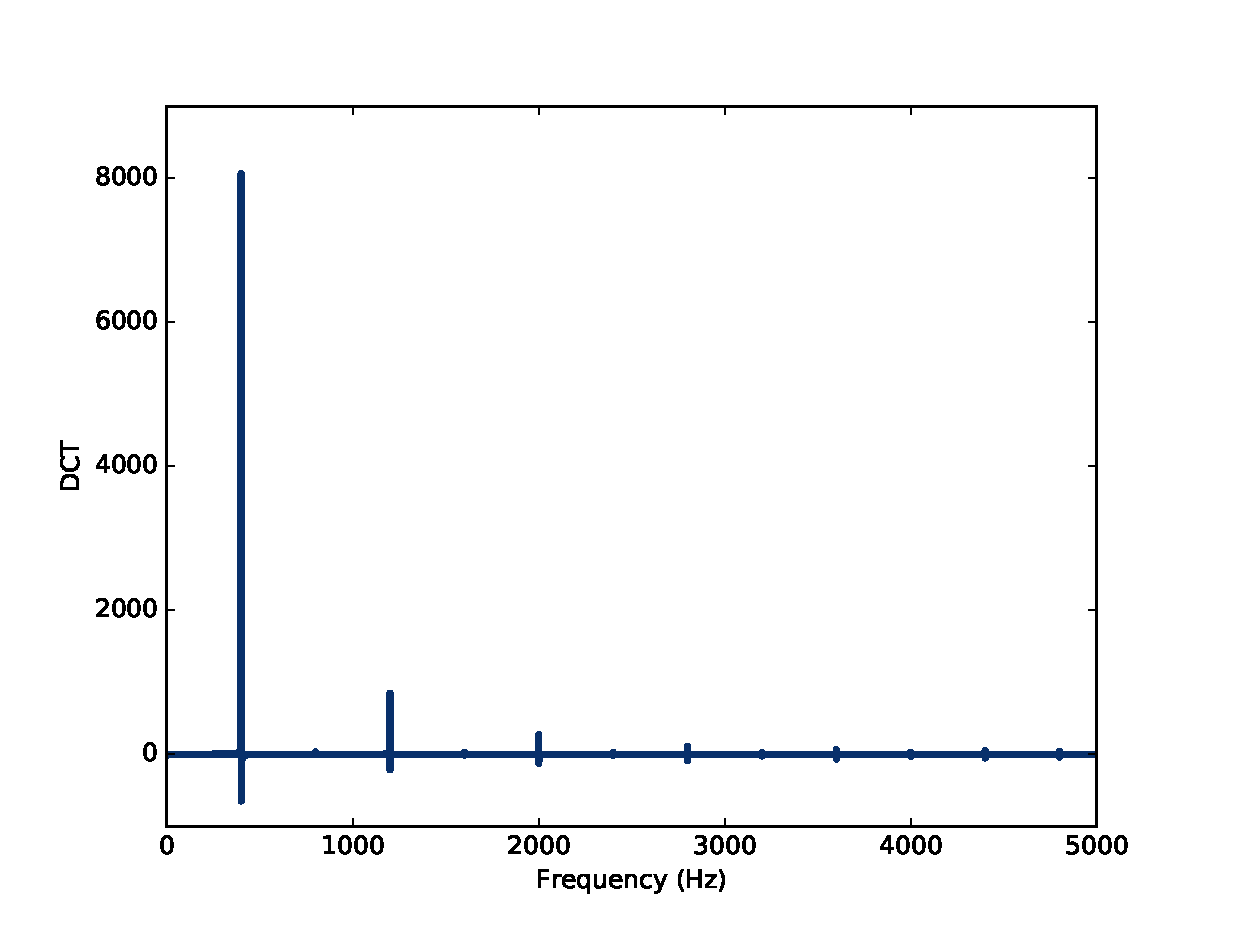
\includegraphics[height=2.5in]{figs/dct1.eps}}
\caption{DCT of a triangle signal at 400 Hz, sampled at 10 kHz.}
\label{fig.dct1}
\end{figure}

{\tt thinkdsp} provides a Dct class that encapsulates the
DCT in the same way the Spectrum class encapsulates the FFT.
To make a Dct object, you can invoke \verb"make_dct" on a Wave.

\begin{verbatim}
signal = thinkdsp.TriangleSignal(freq=400)
wave = signal.make_wave(duration=1.0, framerate=10000)
dct = wave.make_dct()
dct.plot()
\end{verbatim}

The result is the DCT of a triangle wave at 400 Hz, shown in
Figure~\ref{dct1}.  The values of the DCT can be positive or negative;
a negative value in the DCT corresponds to a negated cosine or,
equivalently, to a cosine shifted by 180 degrees.

\verb"make_dct" uses DCT-II, which is the most common type of DCT,
provided by {\tt scipy.fftpack}.

\begin{verbatim}
import scipy.fftpack

# class Wave:
    def make_dct(self):
        N = len(self.ys)
        hs = scipy.fftpack.dct(self.ys, type=2)
        fs = (0.5 + np.arange(N)) / 2
        return Dct(hs, fs, self.framerate)
\end{verbatim}

The results from {\tt dct} are stored in {\tt hs}.  The corresponding
frequencies, computed as in Section~\ref{dctiv}, are stored in {\tt fs}.
And then both are used to initialize the Dct object.

Dct provides \verb"make_wave", which performs the inverse DCT.
We can test it like this:

\begin{verbatim}
wave2 = dct.make_wave()
max(abs(wave.ys-wave2.ys))
\end{verbatim}

The biggest difference between {\tt ys1} and {\tt ys2} is about {\tt
  1e-16}, which is what we expect due to floating-point errors.

\verb"make_wave" uses {\tt scipy.fftpack.idct}: 

\begin{verbatim}
# class Dct
    def make_wave(self):
        n = len(self.hs)
        ys = scipy.fftpack.idct(self.hs, type=2) / 2 / n
        return Wave(ys, framerate=self.framerate) 
\end{verbatim}

Be default, the inverse DCT doesn't normalize the result, so we have
to divide through by $2N$.


\section{Exercises}

For the following exercises, I provide some starter code in
{\tt chap06starter.ipynb}.
Solutions are in {\tt chap06soln.ipynb}.

\begin{exercise}
In this chapter I claim that {\tt analyze1} takes time proportional
to $n^3$ and {\tt analyze2} takes time proportional to $n^2$.  To
see if that's true, run them on a range of input sizes and time
them.  In IPython, you can use the ``magic command'' \verb"%timeit".

If you plot run time versus input size on a log-log scale, you
should get a straight line with slope 3 for  {\tt analyze1} and
slope 2 for {\tt analyze2}.

You also might want to test \verb"dct_iv"
and {\tt scipy.fftpack.dct}.

\end{exercise}


\begin{exercise}
One of the major applications of the DCT is compression for both
sound and images.  In its simplest form, DCT-based compression
works like this:

\begin{enumerate}

\item Break a long signal into segments.

\item Compute the DCT of each segment.

\item Identify frequency components with amplitudes so low they are
  inaudible, and remove them.  Store only the frequencies and
  amplitudes that remain.

\item To play back the signal, load the frequencies and amplitudes
  for each segment and apply the inverse DCT.

\end{enumerate}

Implement a version of this algorithm and apply it to a recording
of music or speech.  How many components can you eliminate before
the difference is perceptible?

In order to make this method practical, you need some way to store a
sparse array; that is, an array where most of the elements are zero.
NumPy provides several implementations of sparse arrays, which you can
read about at
\url{http://docs.scipy.org/doc/scipy/reference/sparse.html}.
\end{exercise}


\begin{exercise}
In the repository for this book you will find an IPython notebook
called \verb"phase.ipynb" that the effect of phase on sound
perception.
Read through this notebook and run the examples.  
Choose another segment of sound and run the same experiments.
Can you find any general relationships between the phase structure
of a sound and how we perceive it?
\end{exercise}




\chapter{Discrete Fourier Transform}
\label{dft}

We've been using the discrete Fourier transform (DFT) since
Chapter~\ref{sounds}, but I haven't explained how it works.  Now is
the time.

If you understand the discrete cosine transform (DCT), you will
understand the DFT.  The only difference is that instead of using the
cosine function, we'll use the complex exponential function.  I'll
start by explaining complex exponentials, then I'll follow the
same progression as in Chapter~\ref{dct}:

\begin{enumerate}

\item We'll start with the synthesis
  problem: given a set of frequency components and their amplitudes,
  how can we construct a signal?  The synthesis problem is 
  equivalent to the inverse DFT.

\item Then I'll rewrite the synthesis problem in the form of matrix
  multiplication using NumPy arrays.

\item Next we'll solve the analysis problem, which is equivalent to
  the DFT: given a signal, how to we find the amplitude and phase
  offset of its frequency components?

\item Finally, we'll use linear algebra to find a more efficient way
  to compute the DFT.

\end{enumerate}

The code for this chapter is in {\tt chap07.ipynb}, which is in the
repository for this book (see Section~\ref{code}).
You can also view it at \url{http://tinyurl.com/thinkdsp07}.


\section{Complex exponentials}

One of the more interesting moves in mathematics is the generalization
of an operation from one type to another.  For example, factorial is a
function that operates on integers; the natural definition for
factorial of $n$ is the product of all integers from 1 to $n$.

If you are of a certain inclination, you might wonder how to compute
the factorial of a non-integer like 3.5.  Since the natural definition
doesn't apply, you might look for other ways to compute the factorial
function, ways that would work with non-integers.

In 1730, Leonhard Euler found one, a generalization of the factorial
function that we know as the gamma function (see
\url{http://en.wikipedia.org/wiki/Gamma_function}).

Euler also found one of the most useful generalizations in applied
mathematics, the complex exponential function.

The natural definition of exponentiation is repeated multiplication.
For example, $\phi^3 = \phi \cdot \phi \cdot \phi$.  But this
definition doesn't apply to non-integer exponents.

However, exponentiation can also be expressed as a power series:
%
\[ e^\phi = 1 + \phi + \phi^2/2! + \phi^3/3! + ... \]
%
This definition works with real numbers, imaginary numbers and, by a simple
extension, with complex numbers.  Applying this definition
to a pure imaginary number, $i\phi$, we get
%
\[ e^{i\phi} = 1 + i\phi - \phi^2/2! - i\phi^3/3! + ... \]
%
By rearranging terms, we can show that this is equivalent to:
%
\[ e^{i\phi} = \cos \phi + i \sin \phi \]
%
You can see the derivation at
\url{http://en.wikipedia.org/wiki/Euler's_formula}.

This formula
implies that $e^{i\phi}$ is a complex number with magnitude 1; if you
think of it as a point in the complex plane, it is always on the unit
circle.  And if you think of it as a vector, the angle in radians
between the vector and the positive x-axis is the argument, $\phi$.

In the case where the exponent is a complex number, we have:
%
\[ e^{a + i\phi} = e^a e^{i\phi} = A e^{i\phi} \]
%
where $A$ is a real number that indicates amplitude and
$e^{i\phi}$ is a unit complex number that indicates angle.

NumPy provides a version of {\tt exp} that works with complex numbers:

\begin{verbatim}
>>> phi = 1.5
>>> z = np.exp(1j * phi)
>>> z
(0.0707+0.997j)
\end{verbatim}

Python uses {\tt j} to represent the imaginary unit, rather
than {\tt i}.  A number ending in {\tt j} is considered imaginary,
so {\tt 1j} is just $i$.

When the argument to {\tt np.exp} is imaginary or complex, the
result is a complex number; specifically, a {\tt np.complex128},
which is represented by two 64-bit floating-point numbers.
In this example, the result is {\tt 0.0707+0.997j}.  

Complex numbers have attributes {\tt real} and {\tt imag}:

\begin{verbatim}
>>> z.real
0.0707
>>> z.imag
0.997
\end{verbatim}

To get the magnitude, you can use the built-in function {\tt abs}
or {\tt np.absolute}:

\begin{verbatim}
>>> abs(z)
1.0
>>> np.absolute(z)
1.0
\end{verbatim}

To get the angle, you can use {\tt np.angle}:

\begin{verbatim}
>>> np.angle(z)
1.5
\end{verbatim}

This example confirms that $e^{i \phi}$ is a complex number with
magnitude 1 and angle $\phi$ radians.


\section{Complex signals}

If $\phi(t)$ is a function of time, $e^{i \phi(t)}$ is also a function
of time.  Specifically,
%
\[ e^{i \phi(t)} = \cos \phi(t) + i \sin \phi(t) \]
%
This function describes a quantity that varies in time, so it is
a signal.  Specifically, it is a {\bf complex exponential signal}.

In the special case where the frequency of the signal is constant,
$\phi(t)$ is $2 \pi f t$ and the result is a {\bf complex sinusoid}:
%
\[ e^{i 2 \pi f t} = \cos 2 \pi f t + i \sin 2 \pi f t \]
%
Or more generally, the signal might start at a phase offset
$\phi_0$, yielding
%
\[ e^{i (2 \pi f t + \phi_0)} \]
%
{\tt thinkdsp} provides an implementation of this signal,
{\tt ComplexSinusoid}:

\begin{verbatim}
class ComplexSinusoid(Sinusoid):
 
   def evaluate(self, ts):
        phases = PI2 * self.freq * ts + self.offset
        ys = self.amp * np.exp(1j * phases)
        return ys
\end{verbatim}

{\tt ComplexSinusoid} inherits \verb"__init__" from
{\tt Sinusoid}.  It provides a version of {\tt evaluate}
that is almost identical to {\tt Sinusoid.evaluate}; the
only difference is that it uses {\tt np.exp} instead of
{\tt np.sin}.

The result is a NumPy array of complex numbers:

\begin{verbatim}
>>> signal = thinkdsp.ComplexSinusoid(freq=1, amp=0.6, offset=1)
>>> wave = signal.make_wave(duration=1, framerate=4)
>>> print(wave.ys)
[ 0.324+0.505j -0.505+0.324j -0.324-0.505j  0.505-0.324j]
\end{verbatim}

The frequency of this signal is 1 cycle per second; the amplitude
is 0.6 (in unspecified units); and the phase offset is 1 radian.

This example evaluates the signal at 4 places equally spaced between
0 and 1 second.  The resulting samples are complex numbers.


\section{The synthesis problem}

Just as we did with real sinusoids, we we can create compound signals
by adding up complex sinusoids with different frequencies.  And that
brings us to the complex version of the synthesis problem: given the
frequency and amplitude of each complex component, how do we evaluate the
signal?

The simplest solution is to create {\tt ComplexSinusoid} objects and
add them up.

\begin{verbatim}
def synthesize1(amps, fs, ts):
    components = [thinkdsp.ComplexSinusoid(freq, amp)
                  for amp, freq in zip(amps, fs)]
    signal = thinkdsp.SumSignal(*components)
    ys = signal.evaluate(ts)
    return ys
\end{verbatim}

This function is almost identical to {\tt synthesize1} in
Section~\ref{synth1}; the only difference is that I replaced
{\tt CosSignal} with {\tt ComplexSinusoid}.

Here's an example:

\begin{verbatim}
>>> amps = np.array([0.6, 0.25, 0.1, 0.05])
>>> fs = [100, 200, 300, 400]
>>> framerate = 11025
>>> ts = np.linspace(0, 1, framerate)
>>> ys = synthesize1(amps, fs, ts)
>>> print(ys)
[ 1.000 +0.000e+00j  0.995 +9.093e-02j  0.979 +1.803e-01j ...,
  0.979 -1.803e-01j  0.995 -9.093e-02j  1.000 -5.081e-15j]
\end{verbatim}

At the lowest level, a complex signal is a sequence of complex
numbers.  But how should we interpret it?  We have some intuition for
real signals: they represent quantities that vary in time; for
example, a sound signal represents changes in air pressure.
But nothing we measure in the world yields complex numbers.

\begin{figure}
% dft.py
\centerline{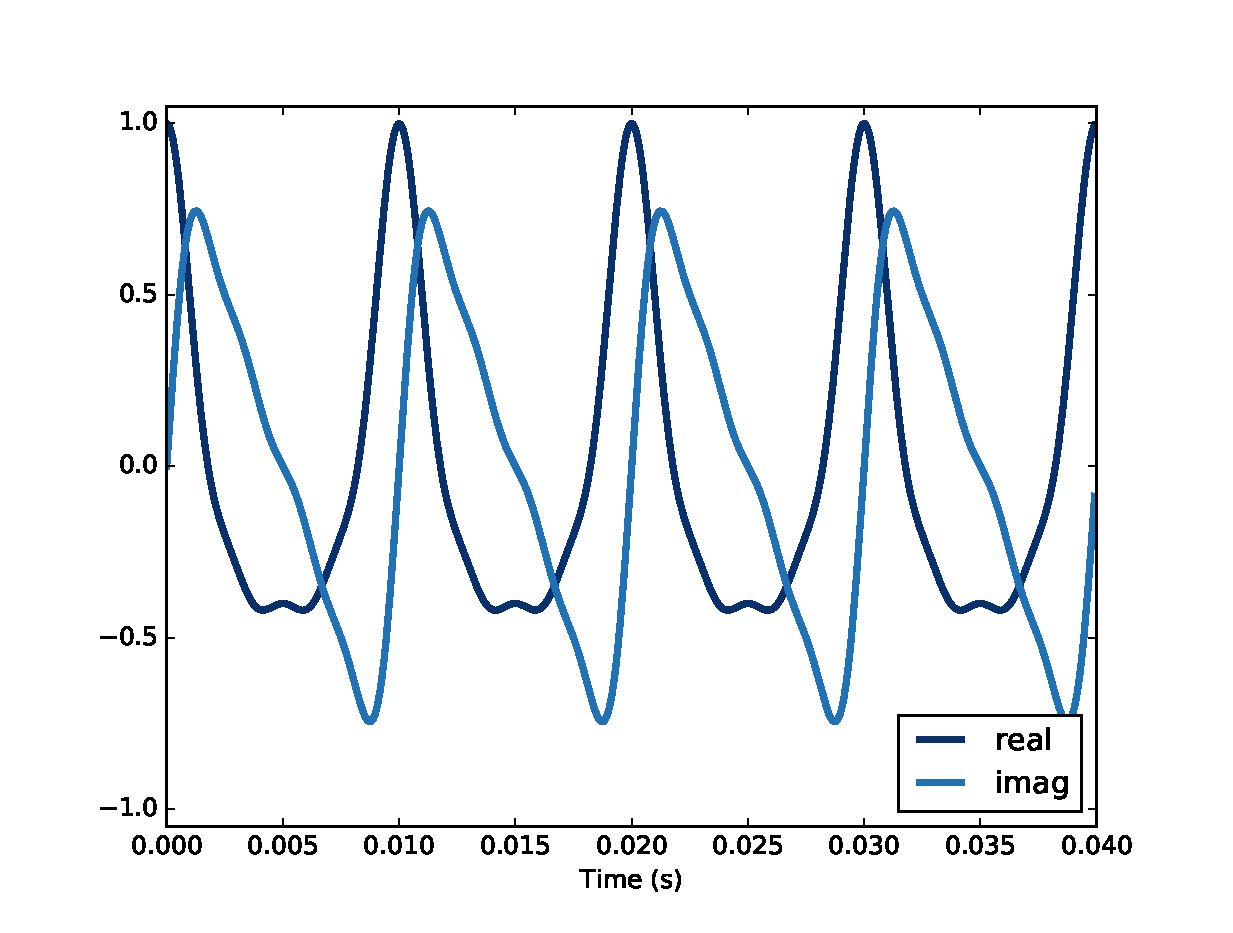
\includegraphics[height=2.5in]{figs/dft1.eps}}
\caption{Real and imaginary parts of a mixture of complex sinusoids.}
\label{fig.dft1}
\end{figure}

So what is a complex signal?  I don't have a satisfying answer to this
question.  The best I can offer is two unsatisfying
answers:

\begin{enumerate}

\item A complex signal is a mathematical abstraction that is useful
  for computation and analysis, but it does not correspond directly
  with anything in the real world.

\item If you like, you can think of a complex signal as a sequence of
  complex numbers that contains two signals as its real and imaginary
  parts.

\end{enumerate}

Taking the second point of view, we can split the previous
signal into its real and imaginary parts:

\begin{verbatim}
    n = 500
    thinkplot.plot(ts[:n], ys[:n].real, label='real')
    thinkplot.plot(ts[:n], ys[:n].imag, label='imag')
\end{verbatim}

Figure~\ref{fig.dft1} shows a segment of the result.  The
real part is a sum of cosines; the imaginary part is
a sum of sines.  Although the waveforms look different, they
contain the same frequency components in the same proportions.
To our ears, they sound the same (in general, we don't hear
phase offsets).


\section{Synthesis with matrices}
\label{synthmat}

As we saw in Section~\ref{synthesis}, we can also express the synthesis
problem in terms of matrix multiplication: 

\begin{verbatim}
PI2 = np.pi * 2

def synthesize2(amps, fs, ts):
    args = np.outer(ts, fs)
    M = np.exp(1j * PI2 * args)
    ys = np.dot(M, amps)
    return ys
\end{verbatim}

Again, {\tt amps} is a NumPy array that contains a sequence of
amplitudes.

{\tt fs} is a sequence containing the frequencies of the
components.  {\tt ts} contains the times where we will evaluate
the signal.

{\tt args} contains the outer product of {\tt ts} and {\tt fs},
with the {\tt ts} running down the rows and the {\tt fs} running
across the columns (you might want to refer back to
Figure~\ref{fig.synthesis}).

Each column of matrix {\tt M} contains a complex sinusoid with
a particular frequency, evaluated at a sequence of {\tt ts}.

When we multiply {\tt M} by the amplitudes, the result is a vector
whose elements correspond to the {\tt ts}; each element is the sum of
several complex sinusoids, evaluated at a particular time.

Here's the example from the previous section again:

\begin{verbatim}
>>> ys = synthesize2(amps, fs, ts)
>>> print(ys)
[ 1.000 +0.000e+00j  0.995 +9.093e-02j  0.979 +1.803e-01j ...,
  0.979 -1.803e-01j  0.995 -9.093e-02j  1.000 -5.081e-15j]
\end{verbatim}

The result is the same.

In this example the amplitudes are real, but they could also be
complex.  What effect does a complex amplitude have on the result?
Remember that we can think of a complex number in two ways: either the
sum of a real and imaginary part, $x + i y$, or the product of a real
amplitude and a complex exponential, $A e^{i \phi_0}$.  Using the
second interpretation, we can see what happens when we multiply
a complex amplitude by a complex sinusoid.  For each frequency, $f$,
we have:
%
\[ A e^{i \phi_0} \cdot e^{i 2 \pi f t} = A e^{i 2 \pi f t + \phi_0} \]
%
Multiplying by $A e^{i \phi_0}$ multiplies the amplitude by $A$
and adds the phase offset $\phi_0$.

\begin{figure}
% dft.py
\centerline{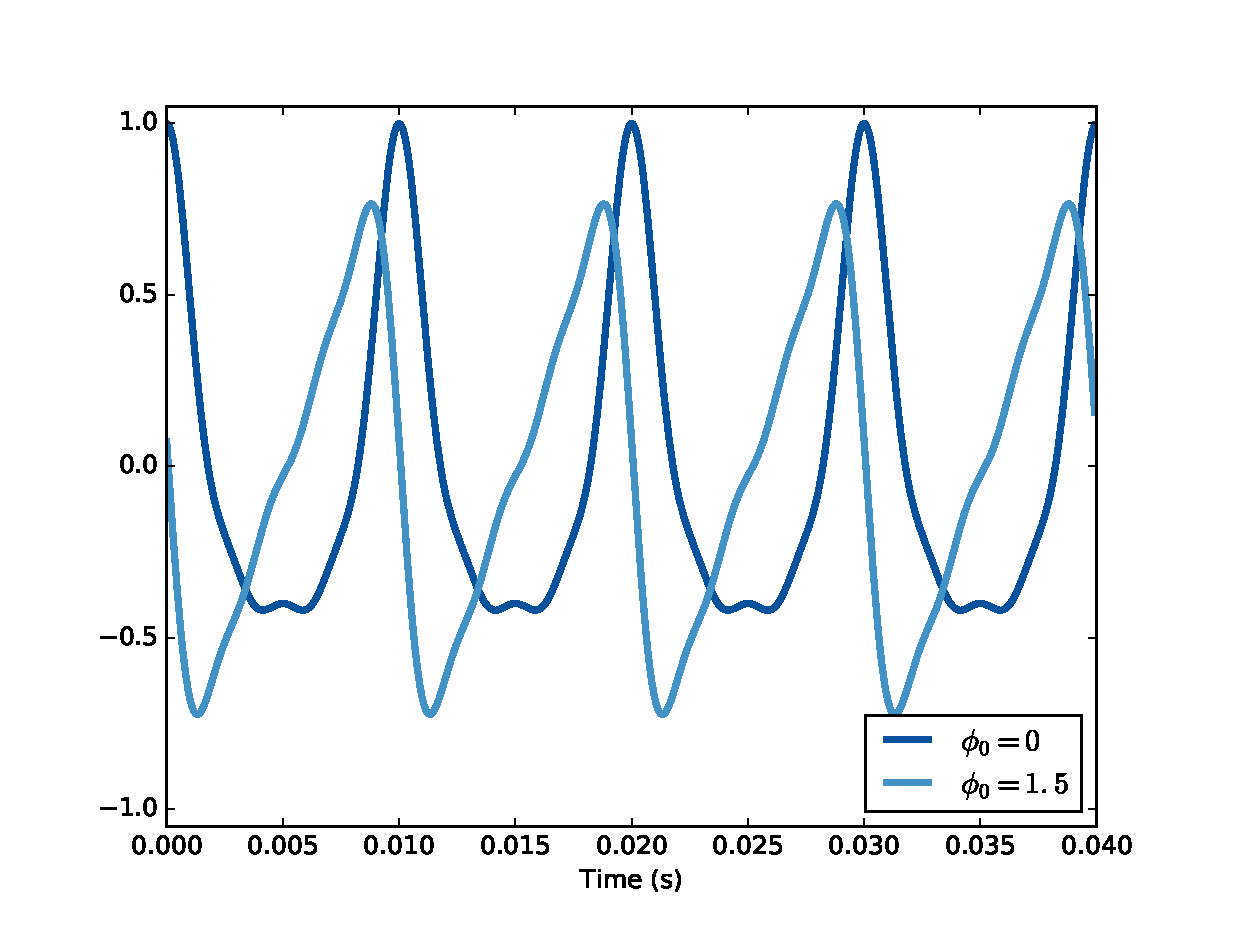
\includegraphics[height=2.5in]{figs/dft2.eps}}
\caption{Real part of two complex signals that differ by a phase
offset.}
\label{fig.dft2}
\end{figure}

We can test that claim by running the previous example with
$\phi_0 = 1.5$ for all frequency components:

\begin{verbatim}
    phi = 1.5
    amps2 = amps * np.exp(1j * phi)
    ys2 = synthesize2(amps2, fs, ts)

    thinkplot.plot(ts[:n], ys.real[:n])
    thinkplot.plot(ts[:n], ys2.real[:n])
\end{verbatim}

Since {\tt amps}
is an array of reals, multiplying by {\tt np.exp(1j * phi)} yields
an array of complex numbers with phase offset {\tt phi} radians, and
the same magnitudes as {\tt amps}.

Figure~\ref{fig.dft2} shows the result.  The phase offset
$\phi_0 = 1.5$ shifts the wave to the left by about one quarter of
a cycle; it also changes the waveform, because the same phase
offset applied to different frequencies changes how the frequency
components line up with each other.

Now that we have the more general solution to the synthesis problem --
one that handles complex amplitudes -- we are ready for the analysis
problem.


\section{The analysis problem}

The analysis problem is the inverse of the synthesis problem: given a
sequence of samples, $y$, and knowing the frequencies
that make up the signal, can we compute the complex amplitudes of the
components, $a$?

As we saw in Section~\ref{analysis}, we can solve this problem by forming
the synthesis matrix, $M$, and solving the system of linear
equations, $M a = y$ for $a$.

\begin{verbatim}
def analyze1(ys, fs, ts):
    args = np.outer(ts, fs)
    M = np.exp(1j * PI2 * args)
    amps = np.linalg.solve(M, ys)
    return amps
\end{verbatim}

{\tt analyze1} takes a (possibly complex) wave array, {\tt ys}, a
sequence of real frequencies, {\tt fs}, and a sequence of real
times, {\tt ts}.  It returns a sequence of complex amplitudes, {\tt
  amps}.

Continuing the previous example, we can confirm that {\tt analyze1}
recovers the amplitudes we started with.  For the linear system
solver to work, {\tt M} has to be square, so we need {\tt ys}, {\tt
  fs} and {\tt ts} to have the same length.  I'll insure that by
slicing {\tt ys} and {\tt ts} down to the length of {\tt fs}:

\begin{verbatim}
>>> n = len(fs)
>>> amps2 = analyze1(ys[:n], fs, ts[:n])
>>> print(amps2)
[ 0.60+0.j  0.25-0.j  0.10+0.j  0.05-0.j]
\end{verbatim}

These are approximately the amplitudes we started with, although
each component has a small imaginary part due to
floating-point errors.


\section{Efficient analysis}

Unfortunately, solving a linear system of equations is slow.  For the
DCT, we were able to speed things up by choosing {\tt fs} and {\tt
  ts} so that {\tt M} is orthogonal.  That way, the inverse of {\tt M}
is the transpose of {\tt M}, and we can compute both DCT and inverse
DCT by matrix multiplication.

We'll do the same thing for the DFT, with one small change.
Since {\tt M} is complex, we need it to be {\bf unitary}, rather
than orthogonal, which means that the inverse of {\tt M} is
the conjugate transpose of {\tt M}, which we can compute by
transposing the matrix and negating the imaginary part of each
element.  See \url{http://en.wikipedia.org/wiki/Unitary_matrix}. 

The NumPy methods {\tt conj} and {\tt transpose} do what we
want.  Here's the code that computes {\tt M} for $N=4$ components:

\begin{verbatim}
>>> N = 4
>>> ts = np.arange(N) / N
>>> fs = np.arange(N)
>>> args = np.outer(ts, fs)
>>> M = np.exp(1j * PI2 * args)
\end{verbatim}

If $M$ is unitary, $M^*M = I$, where $M^*$ is the conjugate transpose
of $M$, and $I$ is the identity matrix.  We can test whether $M$
is unitary like this:

\begin{verbatim}
>>> MstarM = M.conj().transpose().dot(M)
\end{verbatim}

The result, within the tolerance of floating-point error, is
$4 I$, so $M$ is unitary except for an extra factor of $N$,
similar to the extra factor of 2 we found with the DCT.

We can use this result to write a faster version of {\tt analyze1}:

\begin{verbatim}
def analyze2(ys, fs, ts):
    args = np.outer(ts, fs)
    M = np.exp(1j * PI2 * args)
    amps = M.conj().transpose().dot(ys) / N
    return amps
\end{verbatim}

And test it with appropriate values of {\tt fs} and {\tt ts}:

\begin{verbatim}
>>> N = 4
>>> amps = np.array([0.6, 0.25, 0.1, 0.05])
>>> fs = np.arange(N)
>>> ts = np.arange(N) / N
>>> ys = synthesize2(amps, fs, ts)

>>> amps23 = analyze2(ys, fs, ts)
>>> print(amps3)
[ 0.60+0.j  0.25+0.j  0.10-0.j  0.05-0.j]
\end{verbatim}

Again, the result is correct within the tolerance of floating-point
arithmetic.


\section{DFT}
\label{dftsection}

As a function, {\tt analyze2} would be hard to use because it
only works if {\tt fs} and {\tt ts} are chosen correctly.
Instead, I will rewrite it to take just {\tt ys} and compute {\tt freq}
and {\tt ts} itself.

First, I'll make a function to compute the synthesis matrix, $M$:

\begin{verbatim}
def synthesis_matrix(N):
    ts = np.arange(N) / N
    fs = np.arange(N)
    args = np.outer(ts, fs)
    M = np.exp(1j * PI2 * args)
    return M
\end{verbatim}

Then I'll write the function that takes {\tt ys} and returns 
{\tt amps}:

\begin{verbatim}
def analyze3(ys):
    N = len(ys)
    M = synthesis_matrix(N)
    amps = M.conj().transpose().dot(ys) / N
    return amps
\end{verbatim}

We are almost done; {\tt analyze3} computes something very
close to the DFT, with one difference.  The conventional definition
of DFT does not divide by {\tt N}:

\begin{verbatim}
def dft(ys):
    N = len(ys)
    M = synthesis_matrix(N)
    amps = M.conj().transpose().dot(ys)
    return amps
\end{verbatim}

Now we can confirm that my version yields the same result as
FFT:

\begin{verbatim}
>>> dft(ys)
[ 2.4+0.j  1.0+0.j  0.4-0.j  0.2-0.j]
\end{verbatim}

The result is close to {\tt amps * N}.
And here's the version in {\tt np.fft}:

\begin{verbatim}
>>> np.fft.fft(ys)
[ 2.4+0.j  1.0+0.j  0.4-0.j  0.2-0.j]
\end{verbatim}

They are the same, within floating point error.

The inverse DFT is almost the same, except we don't have to transpose
and conjugate $M$, and {\em now} we have to divide through by N:

\begin{verbatim}
def idft(ys):
    N = len(ys)
    M = synthesis_matrix(N)
    amps = M.dot(ys) / N
    return amps
\end{verbatim}

Finally, we can confirm that {\tt dft(idft(amps))} yields {\tt amps}.

\begin{verbatim}
>>> ys = idft(amps)
>>> dft(ys)
[ 0.60+0.j  0.25+0.j  0.10-0.j  0.05-0.j]
\end{verbatim}

If I could go back in time, I might change the definition of
DFT so it divides by $N$ and the inverse DFT doesn't.  That would
be more consistent with my presentation of the synthesis and analysis
problems.

Or I might change the definition so that both operations divide
through by $\sqrt{N}$.  Then the DFT and inverse DFT would be
more symmetric.

But I can't go back in time (yet!), so we're stuck with a slightly
weird convention.  For practical purposes it doesn't really
matter.


\section{The DFT is periodic}

In this chapter I presented the DFT in the form of matrix multiplication.
We compute the synthesis matrix, $M$, and the analysis matrix, $M^*$.
When we multiply $M^{*}$ by the wave array, $y$, each element of the
result is the product of a row from $M^*$ and $y$, which we can
write in the form of a summation:
%
\[ DFT(y)[k] = \sum_n y[n] \exp(-2 \pi i n k / N) \]
%
where $k$ is an index of frequency from
$0$ to $N-1$ and $n$ is an index of time from $0$ to $N-1$.
So $DFT(y)[k]$ is the $k$th element of the DFT of $y$.

Normally we evaluate this summation for $N$ values of $k$, running from
0 to $N-1$.  We {\em could} evaluate it for other values of $k$, but
there is no point, because they start to repeat.  That is, the value at
$k$ is the same as the value at $k+N$ or $k+2N$ or $k-N$, etc.

We can see that mathematically by plugging $k+N$ into the summation:
%
\[ DFT(y)[k+N] = \sum_n y[n] \exp(-2 \pi i n (k+N) / N) \]
%
Since there is a sum in the exponent, we can break it into two parts:
%
\[ DFT(y)[k+N] = \sum_n y[n] \exp(-2 \pi i n k / N)  \exp(-2 \pi i n N / N) \]
%
In the second term, the exponent is always an integer multiple of
$2 \pi$, so the result is always 1, and we can drop it:
%
\[ DFT(y)[k+N] = \sum_n y[n] \exp(-2 \pi i n k / N) \]
%
And we can see that this summation is equivalent to $ DFT(y)[k]$.
So the DFT is periodic, with period $N$.  You will need this result
for one of the exercises below, which asks you to implement the Fast Fourier
Transform (FFT).

As an aside, writing the DFT in the form of a summation provides an
insight into how it works.  If you review the diagram in
Section~\ref{synthesis}, you'll see that each column of the synthesis matrix
is a signal evaluated at a sequence of times.  The analysis matrix is
the (conjugate) transpose of the synthesis matrix, so each {\em row}
is a signal evaluated at a sequence of times.

Therefore, each summation is the correlation of $y$ with one of the
signals in the array (see Section~\ref{dotproduct}).  That is, each
element of the DFT is a correlation that quantifies the similarity of
the wave array, $y$, and a complex exponential at a particular
frequency.


\section{DFT of real signals}

\begin{figure}
% dft.py
\centerline{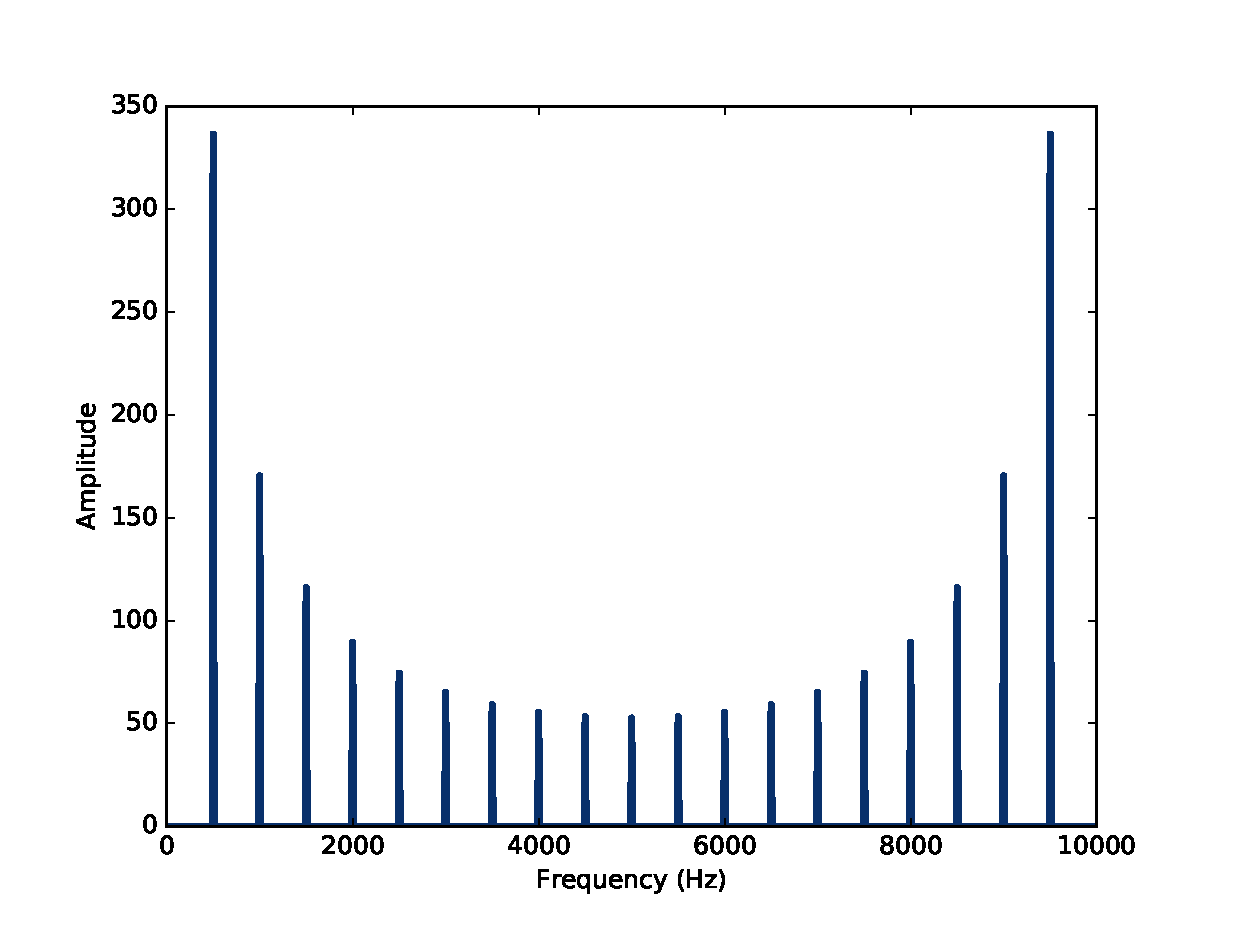
\includegraphics[height=2.5in]{figs/dft3.eps}}
\caption{DFT of a 500 Hz sawtooth signal sampled at 10 kHz.}
\label{fig.dft3}
\end{figure}

The Spectrum class in {\tt thinkdsp} is based on {\tt np.ftt.rfft},
which computes the ``real DFT''; that is, it works with real signals.
But the DFT as presented in this chapter is more general than that; it
works with complex signals.

So what happens when we apply the ``full DFT'' to a real signal?
Let's look at an example:

\begin{verbatim}
>>> signal = thinkdsp.SawtoothSignal(freq=500)
>>> wave = signal.make_wave(duration=0.1, framerate=10000)
>>> hs = dft(wave.ys)
>>> amps = np.absolute(hs)
\end{verbatim}

This code makes a sawtooth wave with frequency 500 Hz, sampled at
framerate 10 kHz.  {\tt hs} contains the complex DFT of the wave;
{\tt amps} contains the amplitude at each frequency.  But what
frequency do these amplitudes correspond to?  If we look at the
body of {\tt dft}, we see:

\begin{verbatim}
>>> fs = np.arange(N)
\end{verbatim}

It's tempting to think that these values are the right frequencies.
The problem is that {\tt dft} doesn't know the sampling rate.  The DFT
assumes that the duration of the wave is 1 time unit, so it thinks the
sampling rate is $N$ per time unit.  In order to interpret the
frequencies, we have to convert from these arbitrary time units back
to seconds, like this:

\begin{verbatim}
>>> fs = np.arange(N) * framerate / N
\end{verbatim}

With this change, the range of frequencies is from 0 to the actual
framerate, 10 kHz.  Now we can plot the spectrum:

\begin{verbatim}
>>> thinkplot.plot(fs, amps)
>>> thinkplot.config(xlabel='frequency (Hz)', 
                     ylabel='amplitude')
\end{verbatim}

Figure~\ref{fig.dft3} shows the amplitude of the signal for each
frequency component from 0 to 10 kHz.  The left half of the figure
is what we should expect: the dominant frequency is at 500 Hz, with
harmonics dropping off like $1/f$.

But the right half of the figure is a surprise.  Past 5000 Hz, the
amplitude of the harmonics start growing again, peaking at 9500 Hz.
What's going on?

The answer: aliasing.  Remember that with framerate 10000 Hz, the
folding frequency is 5000 Hz.  As we saw in Section~\ref{aliasing},
a component at 5500 Hz is indistinguishable from a component
at 4500 Hz.  When we evaluate the DFT at 5500 Hz, we get the same
value as at 4500 Hz.  Similarly, the value at 6000 Hz is the same
as the one at 4000 Hz, and so on.

The DFT of a real signal is symmetric around the folding frequency.
Since there is no additional information past this point, we can
save time by evaluating only the first half of the DFT,
and that's exactly what {\tt np.fft.rfft} does.



\section{Exercises}

Solutions to these exercises are in {\tt chap07soln.ipynb}.


\begin{exercise}
The notebook for this chapter, {\tt chap07.ipynb}, contains
additional examples and explanations.  Read through it and run
the code.
\end{exercise}


\begin{exercise}
In this chapter, I showed how we can express the DFT and inverse DFT
as matrix multiplications.  These operations take time proportional to
$N^2$, where $N$ is the length of the wave array.  That is fast enough
for many applications, but there is a faster
algorithm, the Fast Fourier Transform (FFT), which takes time
proportional to $N \log N$.

The key to the FFT is the Danielson-Lanczos lemma:
%
\[ DFT(y)[n] = DFT(e)[n] + exp(-2 \pi i n / N) DFT(o)[n] \]
%
Where $ DFT(y)[n]$ is the $n$th element of the DFT of $y$; $e$ is a
wave array containing the even elements of $y$, and $o$ contains the
odd elements of $y$.

This lemma suggests a recursive algorithm for the DFT:

\begin{enumerate}

\item Given a wave array, $y$, split it into its even elements, $e$,
  and its odd elements, $o$.

\item Compute the DFT of $e$ and $o$ by making recursive calls.

\item Compute $DFT(y)$ for each value of $n$ using the
  Danielson-Lanczos lemma.

\end{enumerate}

For the base case of this recursion, you could wait until the length
of $y$ is 1.  In that case, $DFT(y) = y$.  Or if the length of $y$
is sufficiently small, you could compute its DFT by matrix multiplication,
possibly using a precomputed matrix.

Hint: I suggest you implement this algorithm incrementally by starting
with a version that is not truly recursive.  In Step 2, instead of
making a recursive call, use {\tt dft}, as defined by
Section~\ref{dftsection}, or {\tt np.fft.fft}.  Get Step 3 working,
and confirm that the results are consistent with the other
implementations.  Then add a base case and confirm that it works.
Finally, replace Step 2 with recursive calls.

One more hint: Remember that the DFT is periodic; you might find {\tt
  np.tile} useful.

You can read more about the FFT at
\url{https://en.wikipedia.org/wiki/Fast_Fourier_transform}.

\end{exercise}


\chapter{Filtering and Convolution}

In this chapter I present one of the most important and useful
ideas related to signal processing: the Convolution Theorem.
But before we can understand the Convolution Theorem, we have to understand
convolution.  I'll start with a simple example, smoothing, and
we'll go from there.

The code for this chapter is in {\tt chap08.ipynb}, which is in the
repository for this book (see Section~\ref{code}).
You can also view it at \url{http://tinyurl.com/thinkdsp08}.


\section{Smoothing}
\label{smoothing}

\begin{figure}
% convolution1.py
\centerline{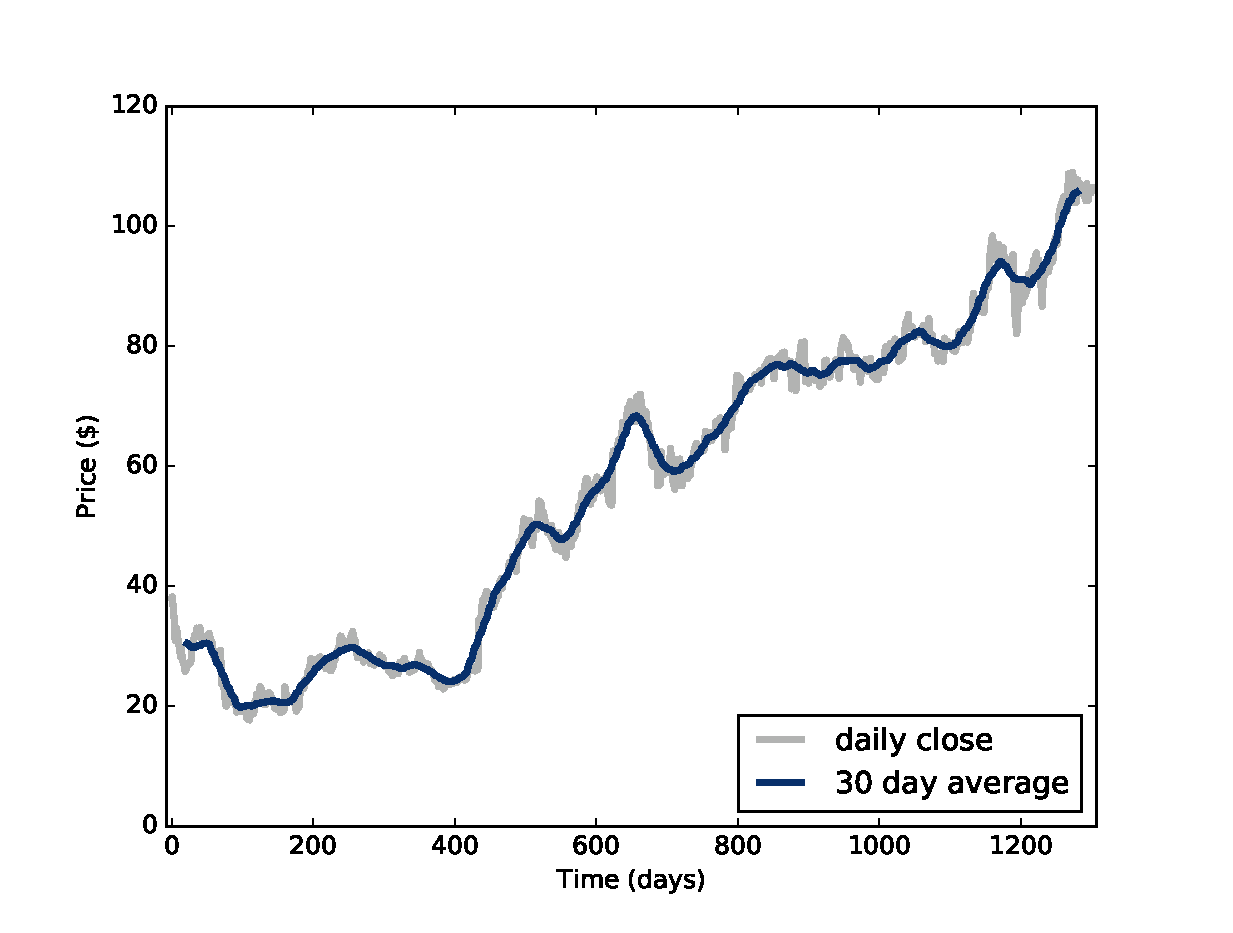
\includegraphics[height=2.5in]{figs/convolution1.eps}}
\caption{Daily closing price of Facebook stock and a 30-day moving
average.}
\label{fig.convolution1}
\end{figure}

Smoothing is an operation that tries to remove short-term variations
from a signal in order to reveal long-term trends.  For example, if
you plot daily changes in the price of a stock, it would look noisy;
a smoothing operator might make it easier to see whether the price
was generally going up or down over time.  

A common smoothing algorithm is a moving average, which computes
the mean of the previous $n$ values, for some value of $n$.

For example, Figure~\ref{fig.convolution1} shows the daily
closing price of Facebook from May 17, 2012 to December 8,
2015.  The gray line
is the raw data, the darker line shows the 30-day moving average.
Smoothing removes the most
extreme changes and makes it easier to see long-term trends.

Smoothing operations also apply to sound signals.  As an example, I'll
start with a square wave at 440 Hz.  As we saw in
Section~\ref{square}, the harmonics of a square wave drop off
slowly, so it contains many high-frequency components.

\begin{verbatim}
>>> signal = thinkdsp.SquareSignal(freq=440)
>>> wave = signal.make_wave(duration=1, framerate=44100)
>>> segment = wave.segment(duration=0.01)
\end{verbatim}

{\tt wave} is a 1-second segment of the signal; {\tt segment}
is a shorter segment I'll use for plotting.

To compute the moving average of this signal, I'll create
a window with 11 elements and normalize it so the elements
add up to 1.

\begin{verbatim}
>>> window = np.ones(11)
>>> window /= sum(window)
\end{verbatim}

Now I can compute the average of the first 11 elements by
multiplying the window by the wave array:

\begin{verbatim}
>>> ys = segment.ys
>>> N = len(ys)
>>> padded = thinkdsp.zero_pad(window, N)
>>> prod = padded * ys
>>> sum(prod)
-1
\end{verbatim}

{\tt padded} is a version of the window with zeros added to
the end so it has the same length as {\tt segment.ys}
{\tt prod} is the product of the window and the wave array.

The sum of the elementwise products is the average of the first 11
elements of the array.  Since these elements are all -1, their average
is -1.

\begin{figure}
% convolution2.py
\centerline{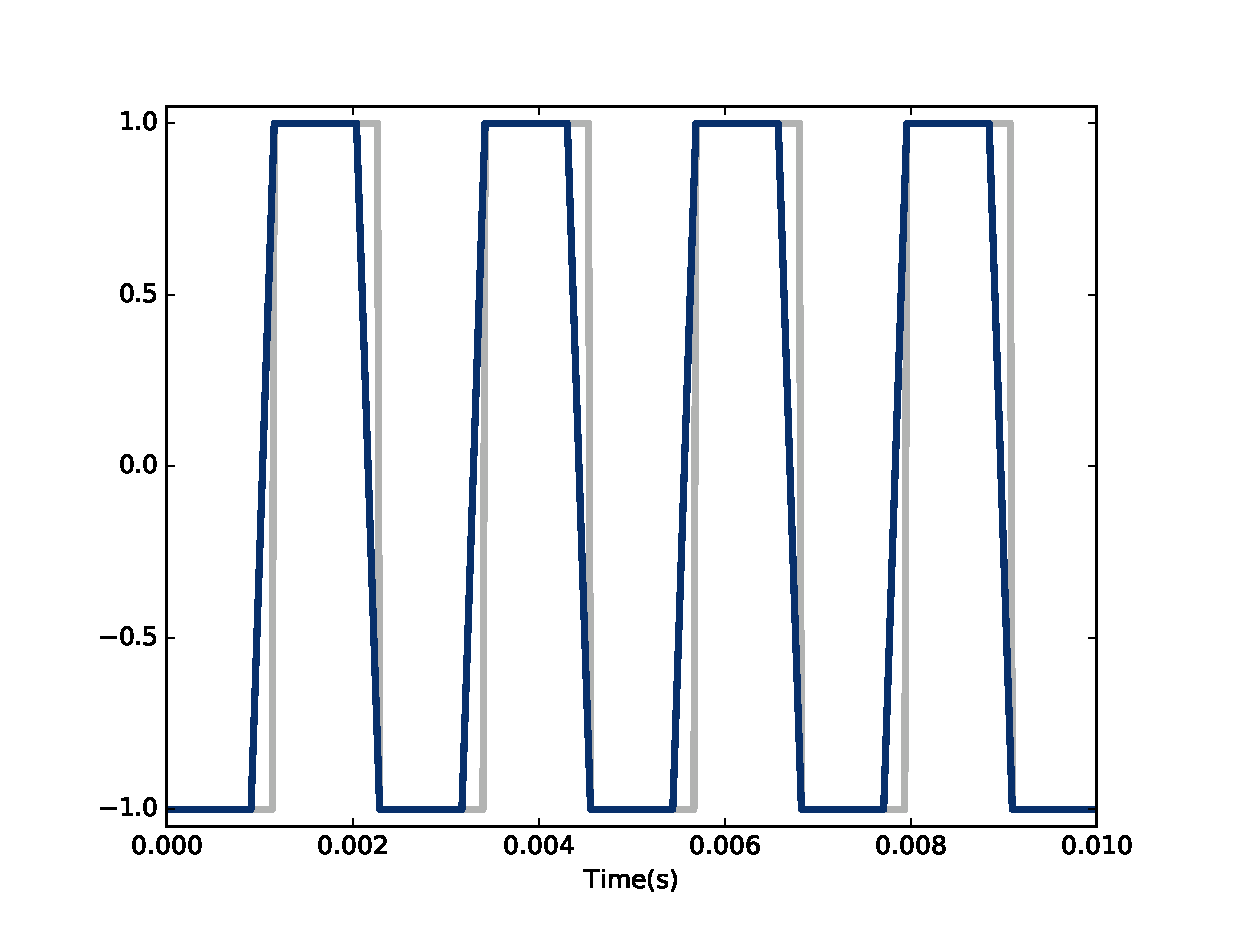
\includegraphics[height=2.5in]{figs/convolution2.eps}}
\caption{A square signal at 400 Hz (gray) and an 11-element
moving average.}
\label{fig.convolution2}
\end{figure}

To compute the next element of the smoothed signal, we shift the
window to the right and compute the average of the next 11 elements of
the wave array, starting with the second.

\begin{verbatim}
>>> rolled = np.roll(rolled, 1)
>>> prod = rolled * ys
>>> sum(prod)
-1
\end{verbatim}

To compute the moving average, we repeat this process and store
the result in an array named {\tt smoothed}:

\begin{verbatim}
>>> smoothed = np.zeros_like(ys)
>>> rolled = padded
>>> for i in range(N):
        smoothed[i] = sum(rolled * ys)
        rolled = np.roll(rolled, 1)
\end{verbatim}

{\tt rolled} is a copy of {\tt padded} that gets shifted to
the right by one element each time through the loop.  Inside
the loop, we multiply the segment by {\tt rolled} to select
11 elements, and then add them up.

Figure~\ref{fig.convolution2} shows the result.  The gray line
is the original signal; the darker line is the smoothed signal.
The smoothed signal starts to ramp up when the leading edge of
the window reaches the first transition, and levels off when
the window crosses the transition.  As a result, the transitions
are less abrupt, and the corners less sharp.  If you listen
to the smoothed signal, it sounds less buzzy and slightly muffled.


\section{Convolution}
\label{convolution}

The operation we just computed is called {\bf convolution},
and it is such a common operation that NumPy provides an
implementation that is simpler and faster than my version:

\begin{verbatim}
>>> convolved = np.convolve(ys, window, mode='valid')
>>> smooth2 = thinkdsp.Wave(convolved, framerate=wave.framerate)
\end{verbatim}

{\tt np.convolve} computes the convolution of the wave
array and the window.  The mode flag {\tt valid} indicates
that it should only compute values when the window and the
wave array overlap completely, so it stops when the right
edge of the window reaches the end of the wave array.  Other
than that, the result is the same as in Figure~\ref{fig.convolution2}.

\newcommand{\conv}{\ast}

Actually, there is one other difference.  The loop in the
previous section actually computes {\bf cross-correlation}:
%
\[ (f \star g)[n] = \sum_{m=0}^{N-1} f[m] g[n+m]  \]
%
where $f$ is a wave array with length $N$, $g$ is the window,
and $\star$ is the symbol for cross-correlation.  To
compute the $n$th element of the result, we shift $g$ to
the right, which is why the index is $n+m$.

The definition of convolution is slightly different:
%
\[ (f \conv g)[n] = \sum_{m=0}^{N-1} f[m] g[n-m]  \]
%
The symbol $\conv$ represents convolution.  The difference is in the
index of $g$: $m$ has been negated, so the summation iterates the
elements of $g$ backward (assuming that negative indices wrap around
to the end of the array).

Because the window we used in this example is symmetric,
cross-correlation and convolution yield the same result.  When we use
other windows, we will have to be more careful.

You might wonder why convolution is defined the way it is.  There
are two reasons:

\begin{itemize}

\item This definition comes up naturally for several applications,
especially analysis of signal-processing systems, which is
the topic of Chapter~\ref{systems}.

\item Also, this definition is the basis of the Convolution Theorem,
coming up very soon.

\end{itemize}


\section{The frequency domain}

\begin{figure}
% convolution4.py
\centerline{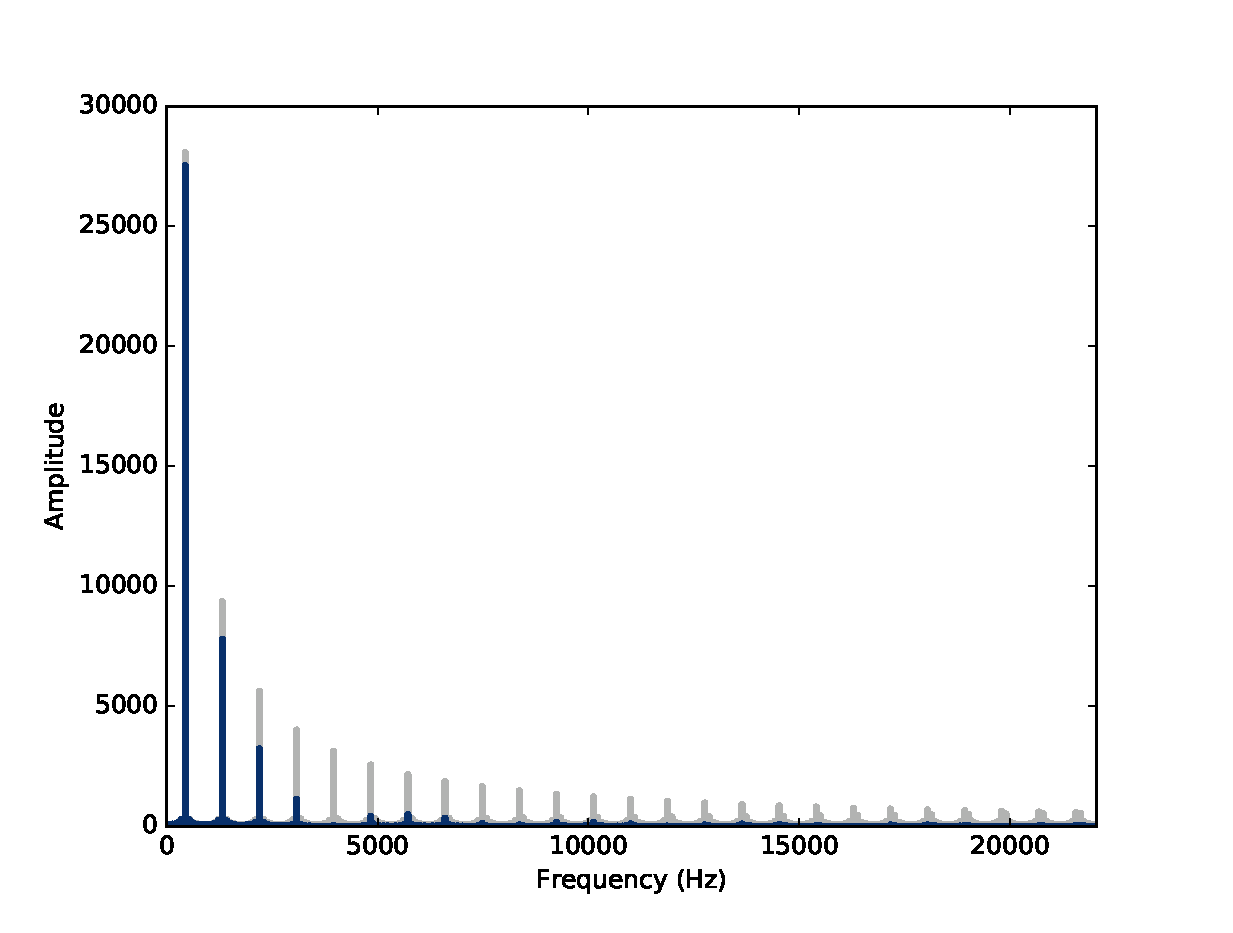
\includegraphics[height=2.5in]{figs/convolution4.eps}}
\caption{Spectrum of the square wave before and after smoothing.}
\label{fig.convolution4}
\end{figure}

Smoothing makes the transitions in a square signal less abrupt,
and makes the sound slightly muffled.  Let's see what effect this
operation has on the spectrum.  First I'll plot the spectrum
of the original wave:

\begin{verbatim}
>>> spectrum = wave.make_spectrum()
>>> spectrum.plot(color=GRAY)
\end{verbatim}

Then the smoothed wave:

\begin{verbatim}
>>> convolved = np.convolve(wave.ys, window, mode='same')
>>> smooth = thinkdsp.Wave(convolved, framerate=wave.framerate)
>>> spectrum2 = smooth.make_spectrum()
>>> spectrum2.plot()
\end{verbatim}

The mode flag {\tt same} indicates that the result should have the
same length as the input.  In this example, it will include a few values
that ``wrap around'', but that's ok for now.

Figure~\ref{fig.convolution4} shows the result.  The fundamental
frequency is almost unchanged; the first few harmonics are
attenuated, and the higher harmonics are almost eliminated.  So
smoothing has the effect of a low-pass filter, which we
saw in Section~\ref{spectrums} and Section~\ref{pink}.

To see how much each component has been attenuated, we can
compute the ratio of the two spectrums:

\begin{verbatim}
>>> amps = spectrum.amps
>>> amps2 = spectrum2.amps
>>> ratio = amps2 / amps    
>>> ratio[amps<560] = 0
>>> thinkplot.plot(ratio)
\end{verbatim}

{\tt ratio} is the ratio of the amplitude before and after 
smoothing.  When {\tt amps} is small, this ratio can be big
and noisy, so for simplicity I set the ratio to 0 except
where the harmonics are.

\begin{figure}
% convolution5.py
\centerline{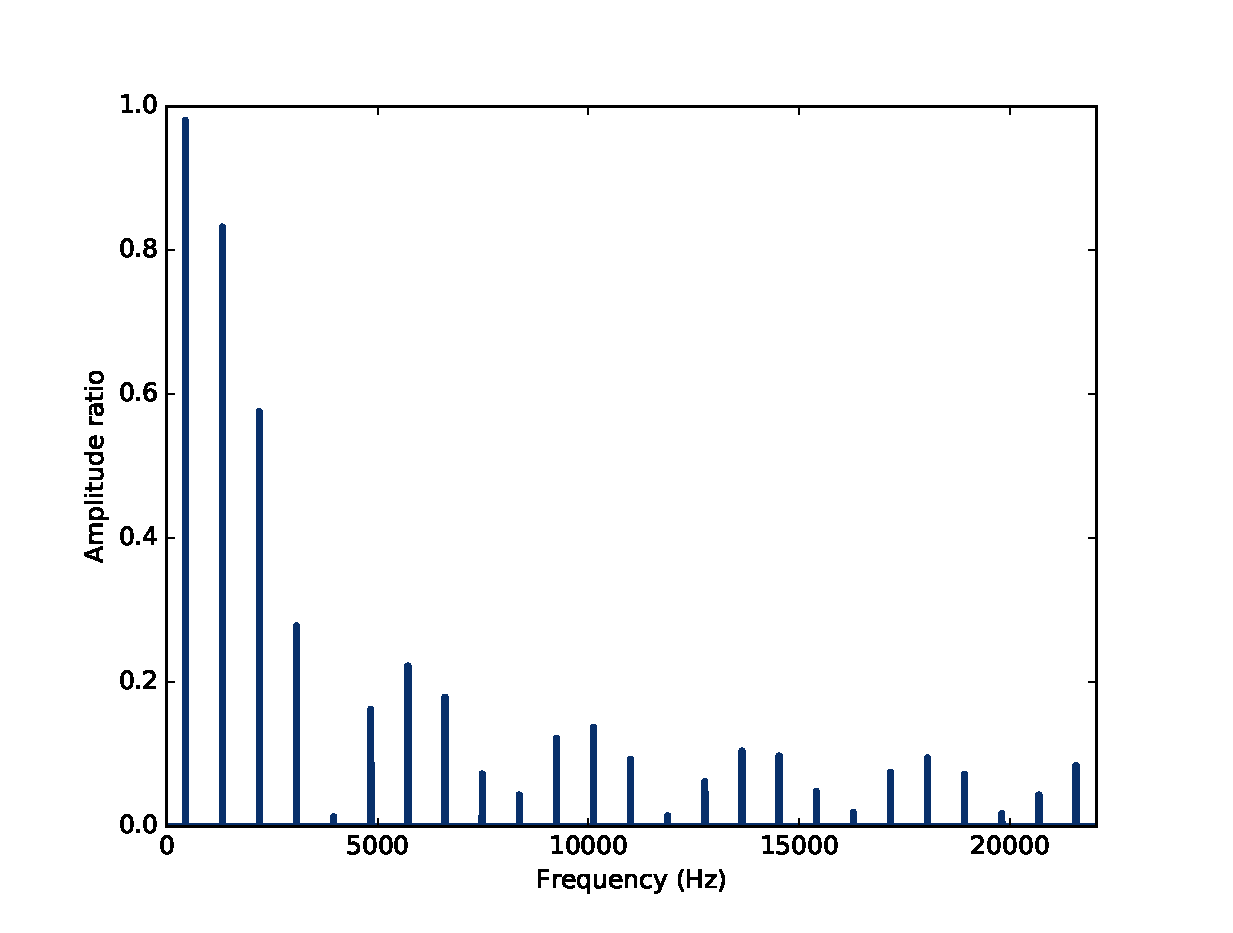
\includegraphics[height=2.5in]{figs/convolution5.eps}}
\caption{Ratio of spectrums for the square wave, before and after smoothing.}
\label{fig.convolution5}
\end{figure}

Figure~\ref{fig.convolution5} shows the result.  As expected, the
ratio is high for low frequencies and drops off at a cutoff frequency
near 4000 Hz.  But there is another feature we did not expect: above
the cutoff, the ratio bounces around between 0 and 0.2.
What's up with that?


\section{The convolution theorem}
\label{convtheorem}

\begin{figure}
% convolution6.py
\centerline{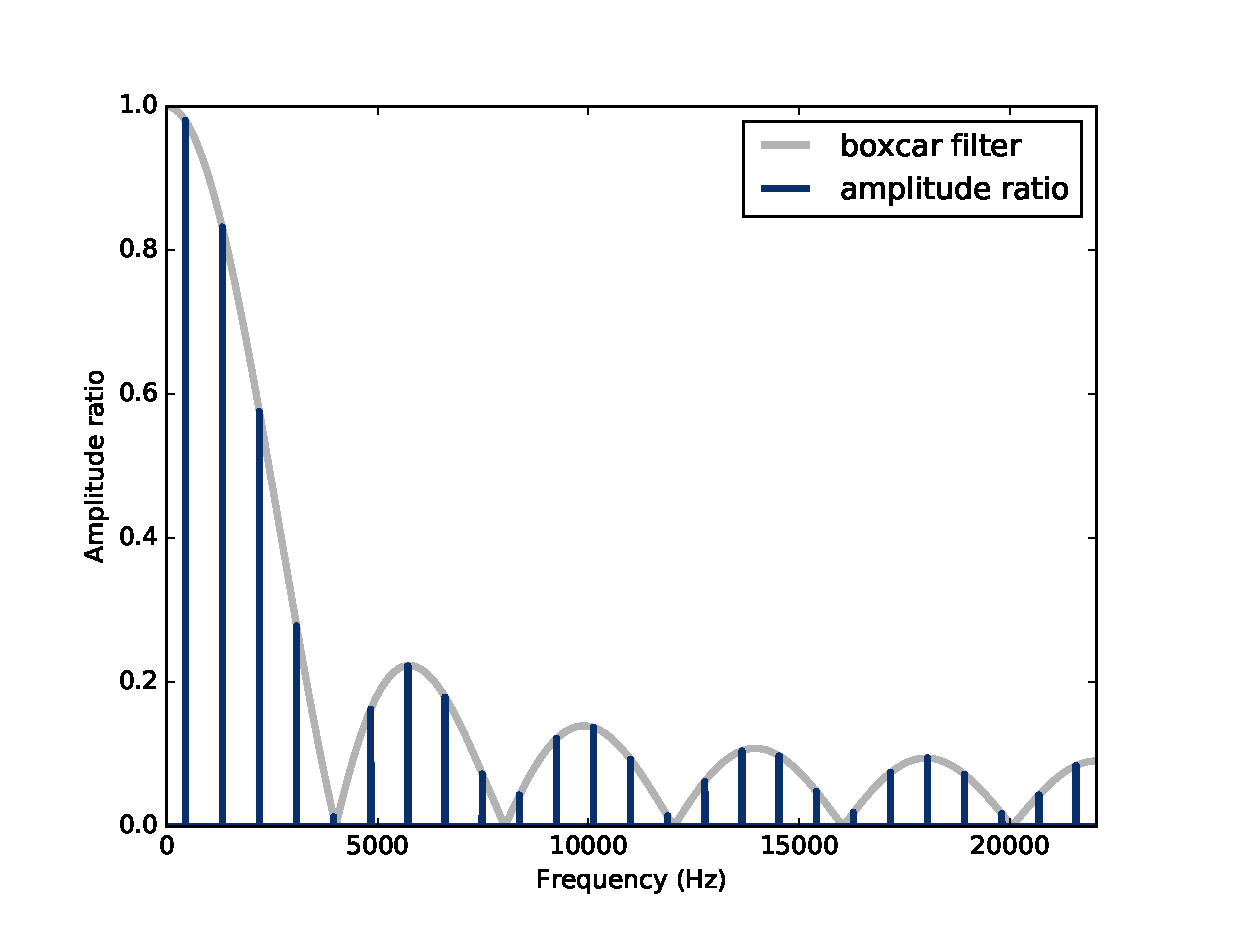
\includegraphics[height=2.5in]{figs/convolution6.eps}}
\caption{Ratio of spectrums for the square wave, before and after
  smoothing, along with the DFT of the smoothing window.}
\label{fig.convolution6}
\end{figure}

\newcommand{\DFT}{\mathrm{DFT}}
\newcommand{\IDFT}{\mathrm{IDFT}}

The answer is the convolution theorem.  Stated mathematically:
%
\[ \DFT(f \conv g) = \DFT(f) \cdot \DFT(g) \]
%
where $f$ is a wave array and $g$ is a window.  In words,
the convolution theorem says that if we convolve $f$ and $g$,
and then compute the DFT, we get the same answer as computing
the DFT of $f$ and $g$, and then multiplying the results
element-wise.  More concisely, convolution in the time
domain corresponds to multiplication in the frequency domain.

And that explains Figure~\ref{fig.convolution5}, because when we
convolve a wave and a window, we multiply the spectrum of
the wave with the spectrum of the window.  To see how that works,
we can compute the DFT of the window:

\begin{verbatim}
    padded = zero_pad(window, N)
    dft_window = np.fft.rfft(padded)
    thinkplot.plot(abs(dft_window))
\end{verbatim}

{\tt padded} contains the window, padded with zeros to be the
same length as {\tt wave}.  \verb"dft_window" contains the
DFT of the smoothing window.

\newcommand{\abs}{\mathrm{abs}}

Figure~\ref{fig.convolution6} shows the result, along with the
ratios we computed in the previous section.  The ratios are
exactly the amplitudes in \verb"dft_window".  Mathematically:
%
\[ \abs(\DFT(f \conv g)) / \abs(\DFT(f)) = \abs(\DFT(g)) \]
%
In this context, the DFT of a window is called a {\bf filter}.
For any convolution window in the time domain, there is a
corresponding filter in the frequency domain.  And for any
filter than can be expressed by element-wise multiplication in
the frequency domain, there is a corresponding window.


\section{Gaussian filter}

\begin{figure}
% convolution7.py
\centerline{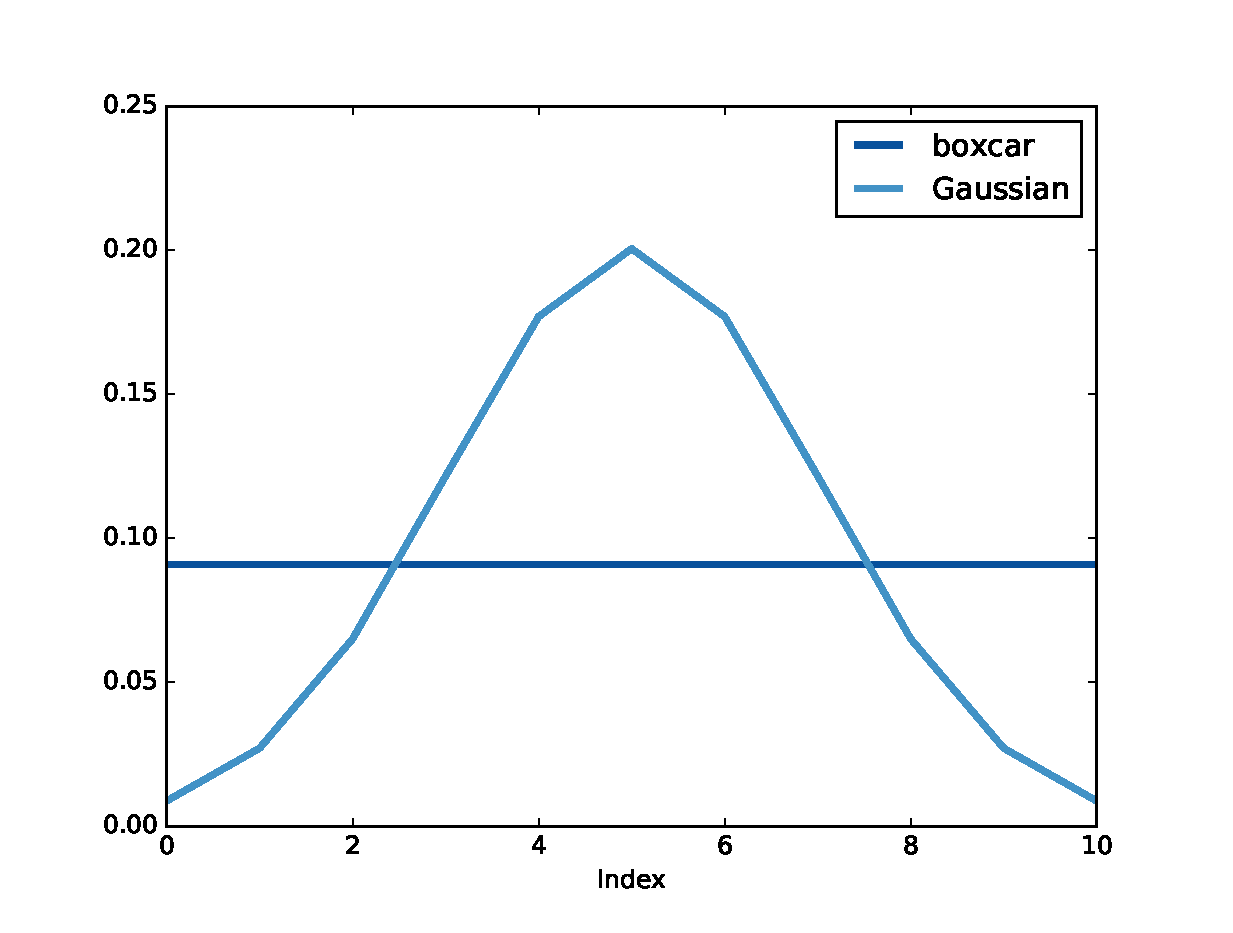
\includegraphics[height=2.5in]{figs/convolution7.eps}}
\caption{Boxcar and Gaussian windows.}
\label{fig.convolution7}
\end{figure}

The moving average window we used in the previous section is a
low-pass filter, but it is not a very good one.  The DFT drops off
steeply at first, but then it bounces around.  Those bounces are
called {\bf sidelobes}, and they are there because the moving average
window is like a square wave, so its spectrum contains high-frequency
harmonics that drop off proportionally to $1/f$, which is relatively
slow.

We can do better with a Gaussian window.  SciPy provides functions
that compute many common convolution windows, including {\tt
  gaussian}:

\begin{verbatim}
    gaussian = scipy.signal.gaussian(M=11, std=2)
    gaussian /= sum(gaussian)
\end{verbatim}

{\tt M} is the number of elements in the window; {\tt std}
is the standard deviation of the Gaussian distribution used to
compute it.  Figure~\ref{fig.convolution7} shows the shape
of the window.  It is a discrete approximation of the Gaussian
``bell curve''.  The figure also shows the moving average window
from the previous example, which is sometimes called a
``boxcar'' window because it looks like a rectangular railway car.

\begin{figure}
% convolution.py
\centerline{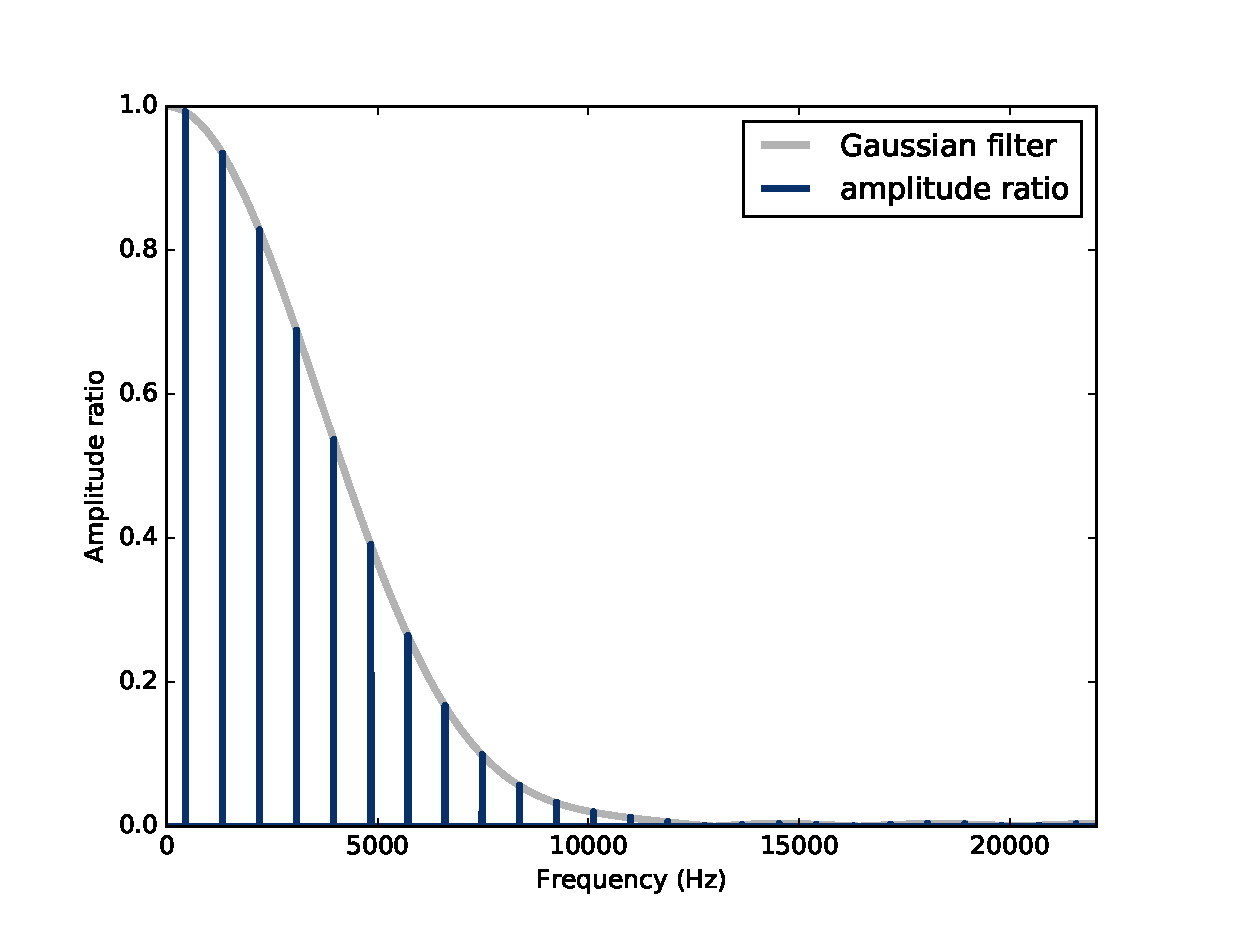
\includegraphics[height=2.5in]{figs/convolution8.eps}}
\caption{Ratio of spectrums before and after Gaussian smoothing, and
  the DFT of the window.}
\label{fig.convolution8}
\end{figure}

I ran the computations from the previous sections again
with this curve, and generated Figure~\ref{fig.convolution8},
which shows the ratio of the spectrums before and after
smoothing, along with the DFT of the Gaussian window. 

As a low-pass filter, Gaussian smoothing is better than a simple
moving average.  After the ratio drops off, it stays low, with almost
none of the sidelobes we saw with the boxcar window.  So it does a
better job of cutting off the higher frequencies.

The reason it does so well is that the DFT of a Gaussian curve is also a
Gaussian curve.  So the ratio drops off in proportion to $\exp(-f^2)$,
which is much faster than $1/f$.


\section{Efficient convolution}
\label{effconv}

One of the reasons the FFT is such an important algorithm is that,
combined with the Convolution Theorem, it provides an efficient
way to compute convolution, cross-correlation, and autocorrelation.

Again, the Convolution Theorem states
%
\[ \DFT(f \conv g) = \DFT(f) \cdot \DFT(g) \]
%
So one way to compute a convolution is:
%
\[ f \conv g = \IDFT(\DFT(f) \cdot \DFT(g)) \]
%
where $IDFT$ is the inverse DFT.  A simple implementation of
convolution takes time proportional to $N^2$; this algorithm,
using FFT, takes time proportional to $N \log N$.

We can confirm that it works by computing the same convolution
both ways.  As an example, I'll apply it to the BitCoin data
shown in Figure~\ref{fig.convolution1}.

\begin{verbatim}
    df = pandas.read_csv('coindesk-bpi-USD-close.csv', 
                         nrows=1625, 
                         parse_dates=[0])
    ys = df.Close.values
\end{verbatim}

This example uses Pandas to read the data from the CSV file (included
in the repository for this book).  If you are not familiar with
Pandas, don't worry: I'm not going to do much with it in this book.
But if you're interested, you can learn more about it in
{\it Think Stats} at \url{http://thinkstats2.com}.

The result, {\tt df}, is a DataFrame, one of the data structures
provided by Pandas.  {\tt ys} is a NumPy array that contains daily
closing prices.

Next I'll create a Gaussian window and convolve it with {\tt ys}:

\begin{verbatim}
    window = scipy.signal.gaussian(M=30, std=6)
    window /= window.sum()
    smoothed = np.convolve(ys, window, mode='valid')
\end{verbatim}

\verb"fft_convolve" computes the same thing using FFT:

\begin{verbatim}
from np.fft import fft, ifft

def fft_convolve(signal, window):
    fft_signal = fft(signal)
    fft_window = fft(window)
    return ifft(fft_signal * fft_window)
\end{verbatim}

We can test it by padding the window to the same length
as {\tt ys} and then computing the convolution:

\begin{verbatim}
    padded = zero_pad(window, N)
    smoothed2 = fft_convolve(ys, padded)
\end{verbatim}

The result has $M-1$ bogus values at the beginning, where $M$ is the
length of the window.  If we slice off the bogus values, the result
agrees with \verb"fft_convolve" with about 12 digits of precision.

\begin{verbatim}
    M = len(window)
    smoothed2 = smoothed2[M-1:]
\end{verbatim}


\section{Efficient autocorrelation}

\begin{figure}
% convolution.py
\centerline{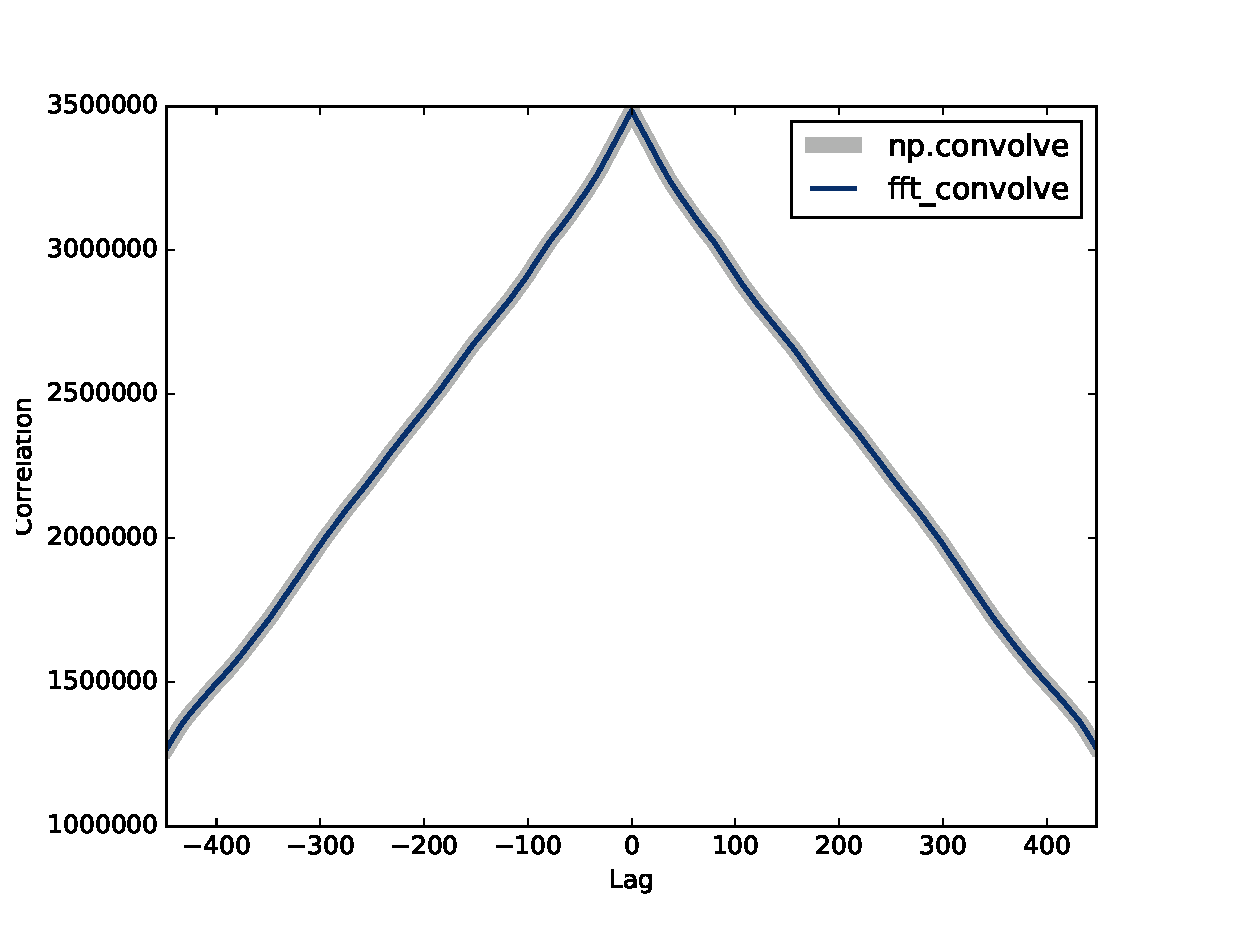
\includegraphics[height=2.5in]{figs/convolution9.eps}}
\caption{Autocorrelation functions computed by NumPy and
  {\tt fft\_correlate}.}
\label{fig.convolution9}
\end{figure}

In Section~\ref{convolution} I presented definitions of
cross-correlation and convolution, and we saw that they are
almost the same, except that in convolution the window is
reversed.

Now that we have an efficient algorithm for convolution, we
can also use it to compute cross-correlations and autocorrelations.
Using the data from the previous section, we can compute the
autocorrelation Facebook stock prices:

\begin{verbatim}
corrs = np.correlate(close, close, mode='same')
\end{verbatim}

With {\tt mode='same'}, the result has the same length as {\tt close},
corresponding to lags from $-N/2$ to $N/2-1$.  
The gray line in Figure~\ref{fig.convolution9} shows the result.
Except at {\tt lag=0}, there are no peaks, so there is no apparent
periodic behavior in this signal.  However, the autocorrelation
function drops off slowly, suggesting that this signal resembled
pink noise, as we saw in Section~\ref{autopink}.

To compute autocorrelation using convolution, 
have to zero-pad the signal to double the length. 
This trick is necessary because the FFT is based
on the assumption that the signal is periodic; that is, that it wraps
around from the end to the beginning.  With time-series data like
this, that assumption is invalid.  Adding zeros, and then trimming 
the results, removes the bogus values.

Also, remember that convolution reverse the direction of the window.
In order to cancel that effect, we reverse the direction of the
window before calling \verb"fft_convolve", using {\tt np.flipud},
which flips a NumPy array.  The result is a view of the array,
not a copy, so this operation is fast.

\begin{verbatim}
def fft_autocorr(signal):
    N = len(signal)
    signal = thinkdsp.zero_pad(signal, 2*N)
    window = np.flipud(signal)

    corrs = fft_convolve(signal, window)
    corrs = np.roll(corrs, N//2+1)[:N]
    return corrs
\end{verbatim}

The result from \verb"fft_convolve" has length $2N$.  Of those,
the first and last $N/2$ are valid; the rest are the result of
zero-padding.  To select the valid element, we roll the results
and select the first $N$, corresponding to lags from $-N/2$ to
$N/2-1$.

As shown in Figure~\ref{fig.convolution9} the results from
\verb"fft_autocorr" and {\tt np.correlate} are identical (with
about 9 digits of precision).

Notice that the correlations in Figure~\ref{fig.convolution9} are
large numbers; we could normalize them (between -1 and 1) as shown
in Section~\ref{correlate}.

The strategy we used here for auto-correlation also works for
cross-correlation.  Again, you have to prepare the signals by flipping
one and padding both, and then you have to trim the invalid parts of
the result.  This padding and trimming is a nuisance, but that's why
libraries like NumPy provide functions to do it for you.


\section{Exercises}

Solutions to these exercises are in {\tt chap08soln.ipynb}.

\begin{exercise}
The notebook for this chapter is {\tt chap08.ipynb}.
Read through it and run the code.

It contains an interactive widget that lets you
experiment with the parameters of the Gaussian window to see
what effect they have on the cutoff frequency.

What goes wrong when you increase the width of the Gaussian,
{\tt std}, without increasing the number of elements in the window,
{\tt M}?
\end{exercise}


\begin{exercise}
In this chapter I claimed that the Fourier transform of a Gaussian
curve is also a Gaussian curve.  For discrete Fourier transforms,
this relationship is approximately true.

Try it out for a few examples.  What happens to the Fourier transform
as you vary {\tt std}?
\end{exercise}


\begin{exercise}
If you did the exercises in Chapter~\ref{nonperiodic}, you saw the
effect of the Hamming window, and some of the other windows provided
by NumPy, on spectral leakage.  We can get some insight into the
effect of these windows by looking at their DFTs.

In addition to the Gaussian window we used in this window, create a
Hamming window with the same size.  Zero pad the windows and plot
their DFTs.  Which window acts as a better low-pass filter?  You might
find it useful to plot the DFTs on a log-$y$ scale.

Experiment with a few different windows and a few different sizes.
\end{exercise}



\chapter{Differentiation and Integration}
\label{diffint}

This chapter picks up where the previous chapter left off,
looking at the relationship between windows in the time domain
and filters in the frequency domain.

In particular, we'll look at the effect of a finite difference
window, which approximates differentiation, and the cumulative
sum operation, which approximates integration.

The code for this chapter is in {\tt chap09.ipynb}, which is in the
repository for this book (see Section~\ref{code}).
You can also view it at \url{http://tinyurl.com/thinkdsp09}.


\section{Finite differences}
\label{diffs}

In Section~\ref{smoothing}, we applied a smoothing window to
the stock price of Facebook and found that a smoothing
window in the time domain corresponds to a low-pass filter in
the frequency domain.

In this section, we'll look at daily price changes and
see that computing the difference between successive elements,
in the time domain, corresponds to a high-pass filter.

Here's the code to read the data, store it as a wave, and compute its
spectrum.

\begin{verbatim}
import pandas as pd

names = ['date', 'open', 'high', 'low', 'close', 'volume']
df = pd.read_csv('fb.csv', header=0, names=names)
ys = df.close.values[::-1]
close = thinkdsp.Wave(ys, framerate=1)
spectrum = wave.make_spectrum()
\end{verbatim}

This example uses Pandas to read the CSV file; the
result is a DataFrame, {\tt df}, with columns for the opening
price, closing price, and high and low prices.  I select the closing
prices and save them in a Wave object.
The framerate is 1 sample per day.  

Figure~\ref{fig.diff_int1} shows
this time series and its spectrum.
Visually, the time series resembles Brownian noise (see
Section~\ref{brownian}).
And the spectrum looks like a straight
line, albeit a noisy one.  The estimated slope is -1.9,
which is consistent with Brownian noise.

\begin{figure}
% diff_int.py
\centerline{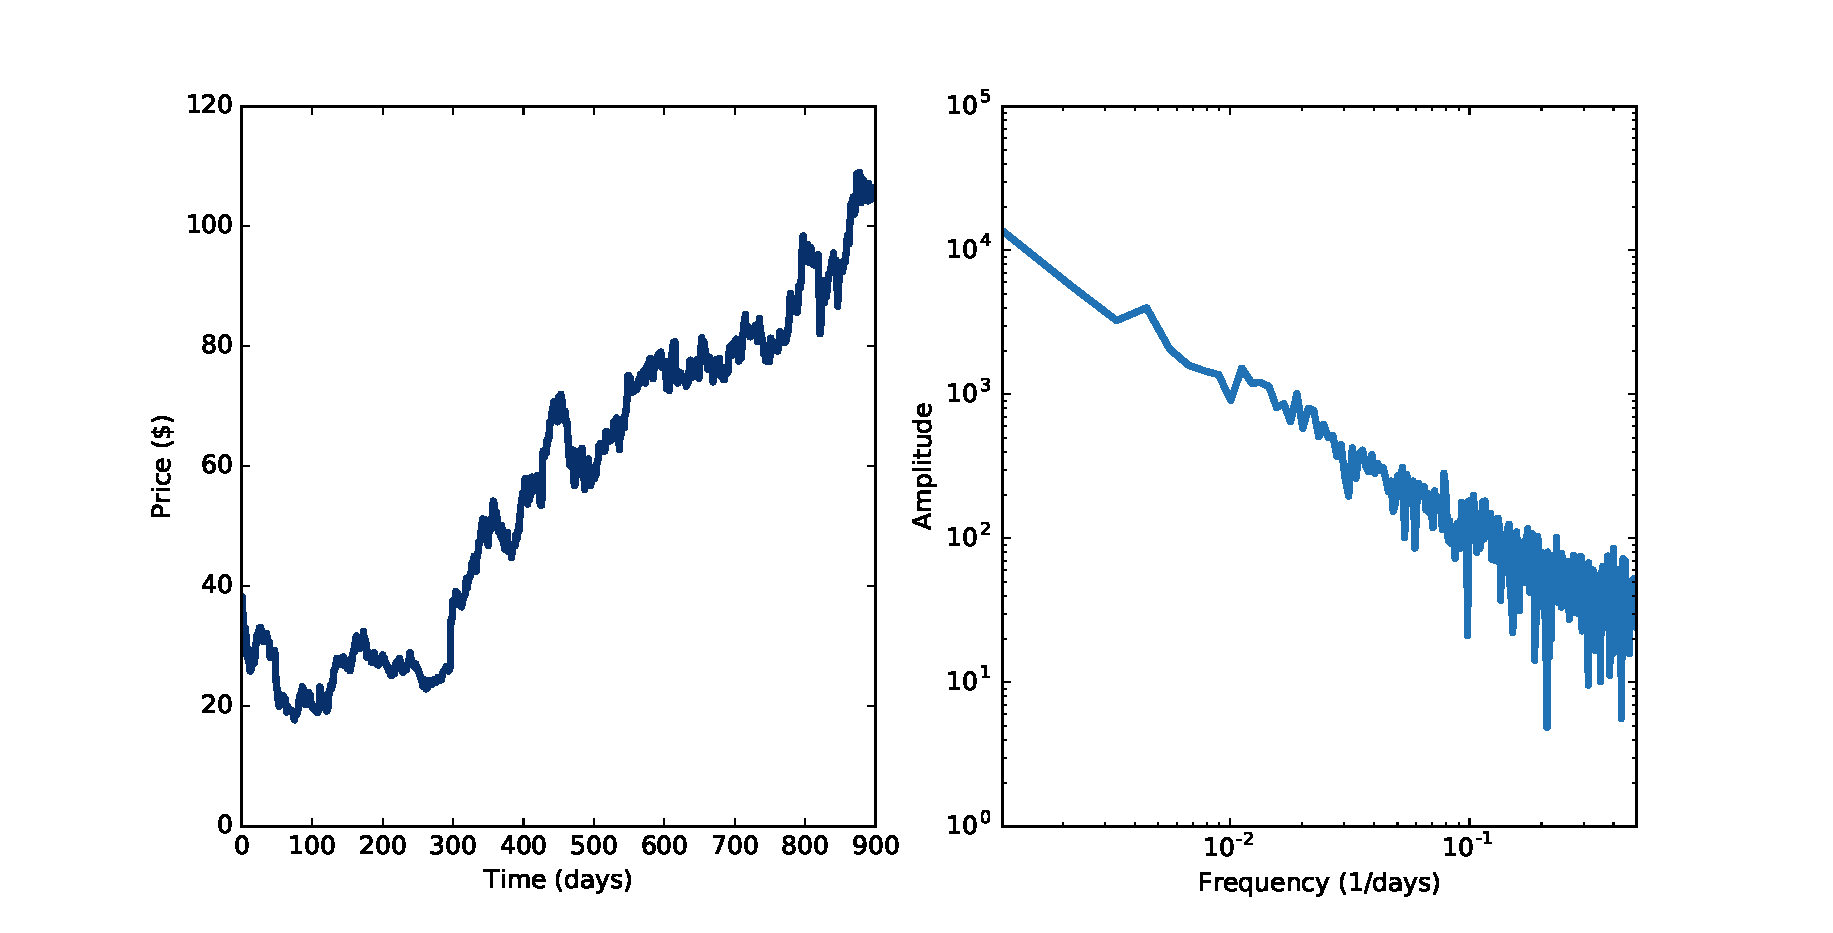
\includegraphics[height=2.5in]{figs/diff_int1.eps}}
\caption{Daily closing price of Facebook and the spectrum of this time
  series.}
\label{fig.diff_int1}
\end{figure}

Now let's compute the daily price change using {\tt np.diff}:

\begin{verbatim}
    diff = np.diff(ys)
    change = thinkdsp.Wave(diff, framerate=1)
    change_spectrum = change.make_spectrum()
\end{verbatim}

Figure~\ref{fig.diff_int2} shows the resulting wave and its spectrum.
The daily changes resemble white noise, and the estimated slope of the
spectrum, -0.06, is near zero, which is what we expect for white
noise.

\begin{figure}
% diff_int2.py
\centerline{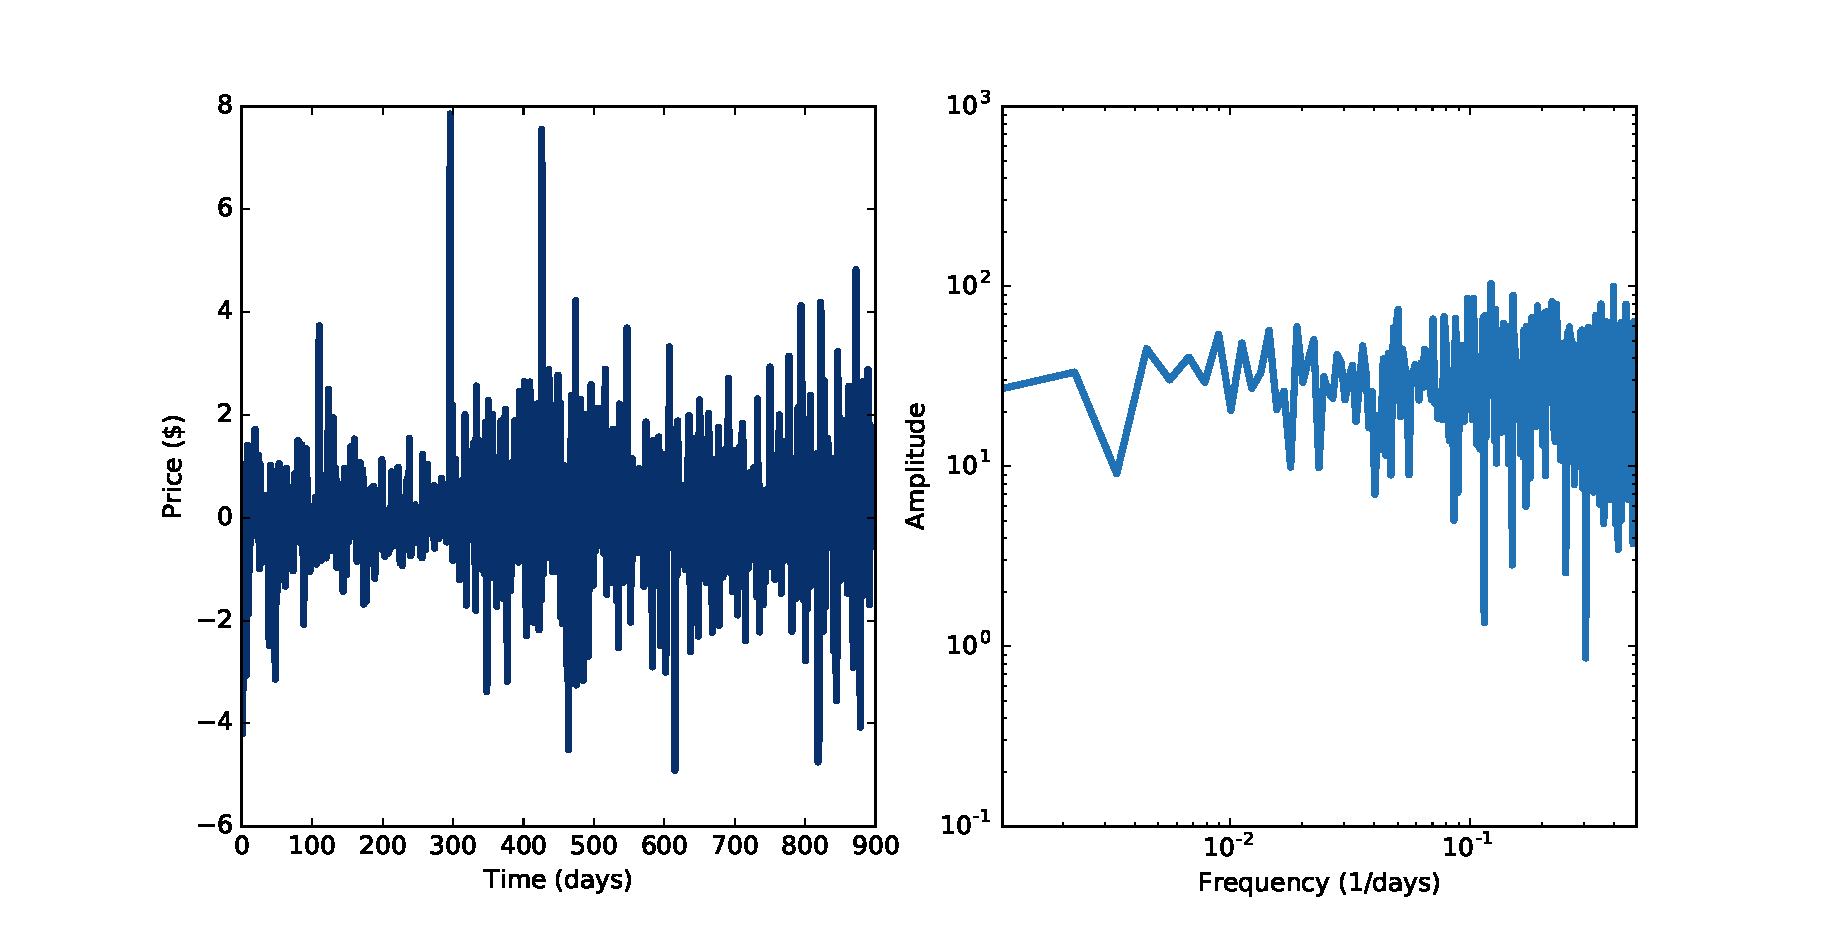
\includegraphics[height=2.5in]{figs/diff_int2.eps}}
\caption{Daily price change of Facebook and the spectrum of this time series.}
\label{fig.diff_int2}
\end{figure}


\section{The frequency domain}

Computing the difference
between successive elements is the same as convolution with
the window {\tt [1, -1]}.
If the order of those elements seems backward,
remember that convolution reverses the window before applying it
to the signal.

We can see the effect of this operation in the frequency domain
by computing the DFT of the window.  

\begin{verbatim}
    diff_window = np.array([1.0, -1.0])
    padded = thinkdsp.zero_pad(diff_window, len(close))
    diff_wave = thinkdsp.Wave(padded, framerate=close.framerate)
    diff_filter = diff_wave.make_spectrum()
\end{verbatim}

\begin{figure}
% diff_int.py
\centerline{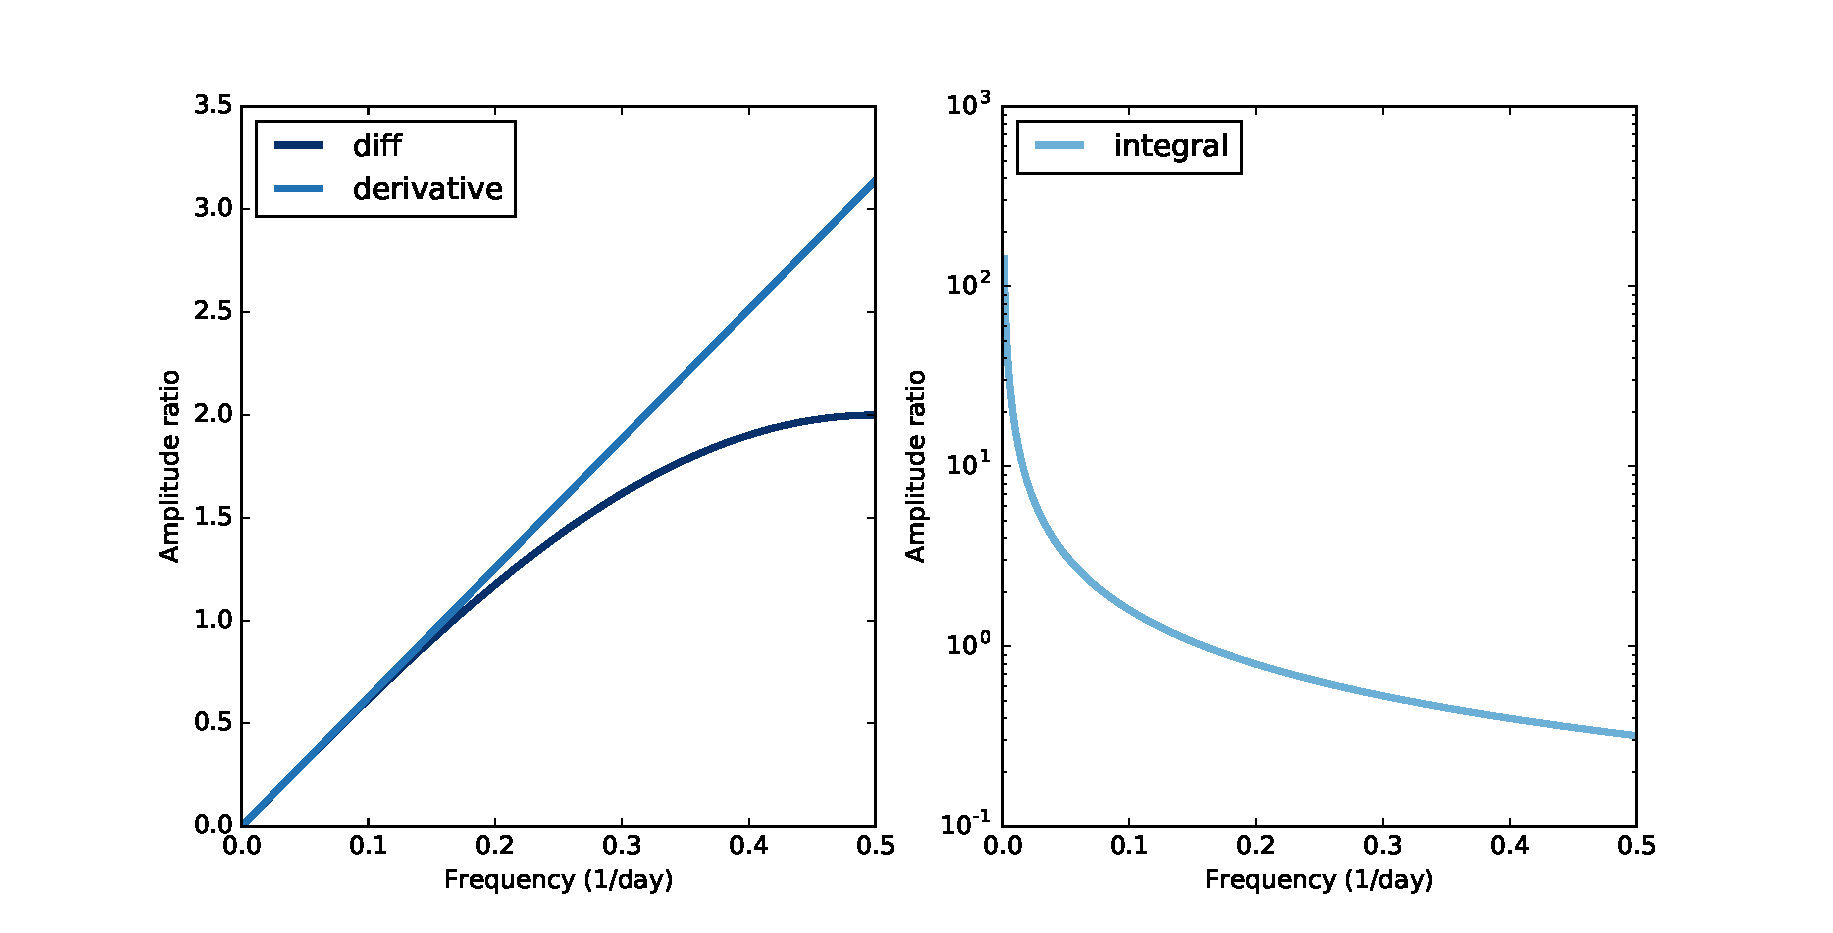
\includegraphics[height=2.5in]{figs/diff_int3.eps}}
\caption{Filters corresponding to the diff and differentiate operators (left) and integration operator (right, log-$y$ scale).}
\label{fig.diff_int3}
\end{figure}

Figure~\ref{fig.diff_int3} shows the result.  The finite difference
window corresponds to a high pass filter: its amplitude increases with
frequency, linearly for low frequencies, and then sublinearly after
that.  In the next section, we'll see why.


\section{Differentiation}
\label{effdiff}

The window we used in the previous section is a
numerical approximation of the first derivative, so the filter
approximates the effect of differentiation.

Differentiation in the time domain corresponds to a simple filter
in the frequency domain; we can figure out what it is with a little
math.

Suppose we have a complex sinusoid with frequency $f$:
%
\[ E_f(t) = e^{2 \pi i f t} \]
%
The first derivative of $E_f$ is
%
\[ \frac{d}{dt} E_f(t) = 2 \pi i f e^{2 \pi i f t} \]
%
which we can rewrite as
%
\[ \frac{d}{dt} E_f(t) = 2 \pi i f E_f(t) \]
%
In other words, taking the derivative of $E_f$ is the same
as multiplying by $2 \pi i f$, which is a complex number
with magnitude $2 \pi f$ and angle $\pi/2$.

We can compute the filter that corresponds to differentiation,
like this:

\begin{verbatim}
    deriv_filter = close.make_spectrum()
    deriv_filter.hs = PI2 * 1j * deriv_filter.fs
\end{verbatim}

I started with the spectrum of {\tt close}, which has the right
size and framerate, then replaced the {\tt hs} with $2 \pi i f$.
Figure~\ref{fig.diff_int3} (left) shows this filter; it is a straight line.

As we saw in Section~\ref{synthmat}, multiplying a complex sinusoid
by a complex number has two effects: it multiplies
the amplitude, in this case by $2 \pi f$, and shifts the phase
offset, in this case by $\pi/2$.

If you are familiar with the language of operators and eigenfunctions,
each $E_f$ is an eigenfunction of the differentiation operator, with the
corresponding eigenvalue $2 \pi i f$.  See
\url{http://en.wikipedia.org/wiki/Eigenfunction}.

If you are not familiar with that language, here's what it
means:

\newcommand{\op}{\mathcal{A}}

\begin{itemize}

\item An operator is a function that takes a function and returns
another function.  For example, differentiation is an operator.

\item A function, $g$, is an eigenfunction of an operator, $\op$, if
applying $\op$ to $g$ has the effect of multiplying the function by
a scalar.  That is, $\op g = \lambda g$.

\item In that case, the scalar $\lambda$ is the eigenvalue that
corresponds to the eigenfunction $g$.

\item A given operator might have many eigenfunctions, each with
a corresponding eigenvalue. 

\end{itemize}

Because complex sinusoids are eigenfunctions of the differentiation
operator, they are easy to differentiate.  All we have to do is
multiply by a complex scalar.

For signals with more than one
component, the process is only slightly harder:

\begin{enumerate}

\item Express the signal as the sum of complex sinusoids.

\item Compute the derivative of each component by multiplication.

\item Add up the differentiated components.

\end{enumerate}

If that process sounds familiar, that's because it is identical
to the algorithm for convolution in Section~\ref{effconv}: compute
the DFT, multiply by a filter, and compute the inverse DFT.

{\tt Spectrum} provides a method that applies the differentiation
filter:

\begin{verbatim}
# class Spectrum:

    def differentiate(self):
        self.hs *= PI2 * 1j * self.fs
\end{verbatim}

We can use it to compute the derivative of the Facebook time series:

\begin{verbatim}
    deriv_spectrum = close.make_spectrum()
    deriv_spectrum.differentiate()
    deriv = deriv_spectrum.make_wave()
\end{verbatim}

\begin{figure}
% diff_int.py
\centerline{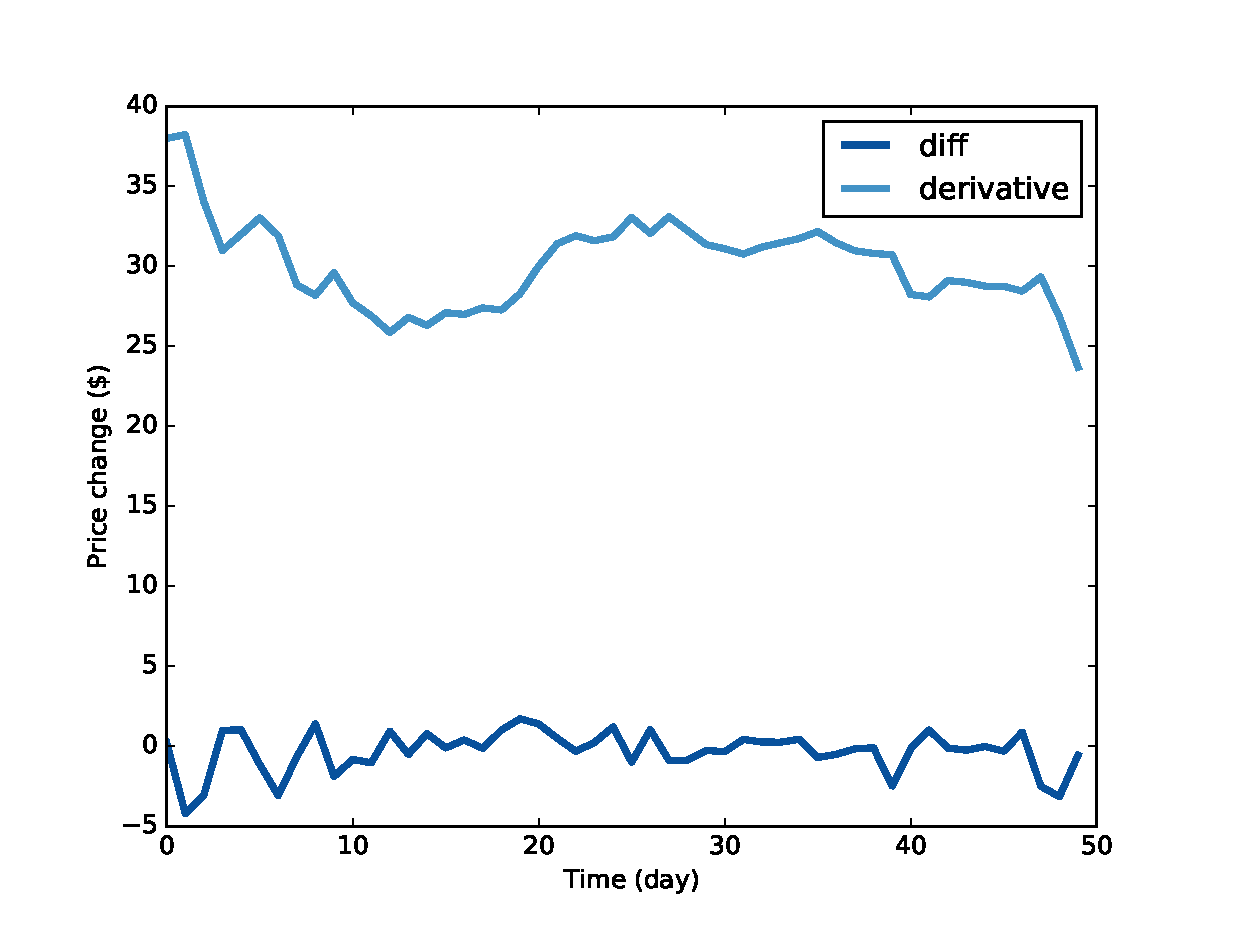
\includegraphics[height=2.5in]{figs/diff_int4.eps}}
\caption{Comparison of daily price changes computed by
{\tt np.diff} and by applying the differentiation filter.}
\label{fig.diff_int4}
\end{figure}

Figure~\ref{fig.diff_int4} compares the daily price changes computed by
{\tt np.diff} with the derivative we just computed.
I selected the first 50 values in the time series so we can see the
differences more clearly.

The derivative is noisier, because it amplifies the high frequency
components more, as shown in Figure~\ref{fig.diff_int3} (left).  Also, the
first few elements of the derivative are very noisy.  The problem
there is that the DFT-based derivative is based on the assumption that
the signal is periodic.  In effect, it connects the last element in
the time series back to the first element, which creates artifacts at
the boundaries.

To summarize, we have shown:

\begin{itemize} 

\item Computing the difference between successive values in a signal
  can be expressed as convolution with a simple window.  The result is
  an approximation of the first derivative.

\item Differentiation in the time domain corresponds to a simple
  filter in the frequency domain.  For periodic signals, the result is
  the first derivative, exactly.  For some non-periodic signals, it
  can approximate the derivative.

\end{itemize}

Using the DFT to compute derivatives is the basis of {\bf spectral
  methods} for solving differential equations (see
\url{http://en.wikipedia.org/wiki/Spectral_method}).

In particular, it is useful for the analysis of linear, time-invariant
systems, which is coming up in Chapter~\ref{systems}.


\section{Integration}

\begin{figure}
% diff_int.py
\centerline{\includegraphics[height=2.5in]{figs/diff_int5.eps}}
\caption{Comparison of the original time series and the integrated
derivative.}
\label{fig.diff_int5}
\end{figure}

In the previous section, we showed that differentiation in the time
domain corresponds to a simple filter in the frequency domain: it
multiplies each component by $2 \pi i f$.  Since integration is
the inverse of differentiation, it also corresponds to a simple
filter: it divides each component by $2 \pi i f$.

We can compute this filter like this:

\begin{verbatim}
    integ_filter = close.make_spectrum()
    integ_filter.hs = 1 / (PI2 * 1j * integ_filter.fs)
\end{verbatim}

Figure~\ref{fig.diff_int3} (right) shows this filter on a log-$y$ scale,
which makes it easier to see.

{\tt Spectrum} provides a method that applies the integration filter:

\begin{verbatim}
# class Spectrum:

    def integrate(self):
        self.hs /= PI2 * 1j * self.fs
\end{verbatim}

We can confirm that the integration filter is correct by applying it
to the spectrum of the derivative we just computed:

\begin{verbatim}
    integ_spectrum = deriv_spectrum.copy()
    integ_spectrum.integrate()
\end{verbatim}

But notice that at $f=0$, we are dividing by 0.  The result in
NumPy is NaN, which is a special floating-point value that
represents ``not a number''.  We can partially deal with this
problem by setting this value to 0 before converting the
spectrum back to a wave:

\begin{verbatim}
    integ_spectrum.hs[0] = 0
    integ_wave = integ_spectrum.make_wave()
\end{verbatim}

Figure~\ref{fig.diff_int5} shows this integrated derivative along with
the original time series.  They are almost identical, but the
integrated derivative has been shifted down.  The problem is that when
we clobbered the $f=0$ component, we set the bias of the signal to 0.
But that should not be surprising; in general, differentiation loses
information about the bias, and integration can't recover it.  In some
sense, the NaN at $f=0$ is telling us that this element is unknown.

\begin{figure}
% diff_int.py
\centerline{\includegraphics[height=2.5in]{figs/diff_int6.eps}}
\caption{A sawtooth wave and its spectrum.}
\label{fig.diff_int6}
\end{figure}

If we provide this ``constant of integration'', the results are
identical, which confirms that this integration filter is the correct
inverse of the differentiation filter.

\section{Cumulative sum}
\label{cumsum}

In the same way that the diff operator approximates differentiation,
the cumulative sum approximates integration.
I'll demonstrate with a Sawtooth signal.

\begin{verbatim}
    signal = thinkdsp.SawtoothSignal(freq=50)
    in_wave = signal.make_wave(duration=0.1, framerate=44100)
\end{verbatim}

Figure~\ref{fig.diff_int6} shows this wave and its spectrum.

{\tt Wave} provides a method that computes the cumulative sum of
a wave array and returns a new Wave object:

\begin{verbatim}
# class Wave:

    def cumsum(self):
        ys = np.cumsum(self.ys)
        ts = self.ts.copy()
        return Wave(ys, ts, self.framerate)
\end{verbatim}

We can use it to compute the cumulative sum of \verb"in_wave":

\begin{verbatim}
    out_wave = in_wave.cumsum()
    out_wave.unbias()
\end{verbatim}

\begin{figure}
% diff_int.py
\centerline{\includegraphics[height=2.5in]{figs/diff_int7.eps}}
\caption{A parabolic wave and its spectrum.}
\label{fig.diff_int7}
\end{figure}

Figure~\ref{fig.diff_int7} shows the resulting wave and its spectrum.
If you did the exercises in Chapter~\ref{harmonics}, this waveform should
look familiar: it's a parabolic signal.

Comparing the spectrum of the parabolic signal to the spectrum of the
sawtooth, the amplitudes of the components drop off more quickly.  In
Chapter~\ref{harmonics}, we saw that the components of the sawtooth
drop off in proportion to $1/f$.  Since the cumulative sum
approximates integration, and integration filters components in
proportion to $1/f$, the components of the parabolic wave drop off in
proportion to $1/f^2$.

We can see that graphically by computing the filter that corresponds
to the cumulative sum:

\begin{verbatim}
    cumsum_filter = diff_filter.copy()
    cumsum_filter.hs = 1 / cumsum_filter.hs
\end{verbatim}

Because {\tt cumsum} is the inverse operation of {\tt diff}, we
start with a copy of \verb"diff_filter", which is the filter
that corresponds to the {\tt diff} operation, and then invert the
{\tt hs}.

\begin{figure}
% diff_int.py
\centerline{\includegraphics[height=2.5in]{figs/diff_int8.eps}}
\caption{Filters corresponding to cumulative sum and integration.}
\label{fig.diff_int8}
\end{figure}

Figure~\ref{fig.diff_int8} shows the filters corresponding to
cumulative sum and integration.  The cumulative sum is a good
approximation of integration except at the highest frequencies,
where it drops off a little faster. 

To confirm that this is the correct filter for the cumulative
sum, we can compare it to the ratio of the spectrum
\verb"out_wave" to the spectrum of \verb"in_wave":

\begin{verbatim}
    in_spectrum = in_wave.make_spectrum()
    out_spectrum = out_wave.make_spectrum()
    ratio_spectrum = out_spectrum.ratio(in_spectrum, thresh=1)
\end{verbatim}

\begin{figure}
% diff_int.py
\centerline{\includegraphics[height=2.5in]{figs/diff_int9.eps}}
\caption{Filter corresponding to cumulative sum and actual ratios of
  the before-and-after spectrums.}
\label{fig.diff_int9}
\end{figure}

And here's the method that computes the ratios:

\begin{verbatim}
    def ratio(self, denom, thresh=1):
        ratio_spectrum = self.copy()
        ratio_spectrum.hs /= denom.hs
        ratio_spectrum.hs[denom.amps < thresh] = np.nan
        return ratio_spectrum
\end{verbatim}

When {\tt denom.amps} is small, the resulting ratio is noisy,
so I set those values to NaN.

Figure~\ref{fig.diff_int8} shows the ratios and the filter
corresponding to the cumulative sum.  They agree, which confirms that
inverting the filter for {\tt diff} yields the filter for {\tt
  cumsum}.

Finally, we can confirm that the Convolution Theorem applies by
applying the {\tt cumsum} filter in the frequency domain:

\begin{verbatim}
    out_wave2 = (in_spectrum * cumsum_filter).make_wave()
\end{verbatim}

Within the limits of floating-point error, \verb"out_wave2" is
identical to \verb"out_wave", which we computed using {\tt cumsum}, so
the Convolution Theorem works!  But note that this demonstration only
works with periodic signals.


\section{Integrating noise}

In Section~\ref{brownian}, we generated Brownian noise by computing the
cumulative sum of white noise.
Now that we understand the effect of {\tt cumsum} in the frequency
domain, we have some insight into the spectrum of Brownian noise.

White noise has equal power at all frequencies, on average.  When we
compute the cumulative sum, the amplitude of each component is divided
by $f$.  Since power is the square of magnitude, the power of each
component is divided by $f^2$.  So on average, the power at frequency
$f$ is proportional to $1 / f^2$:
%
\[ P_f = K / f^2 \]
%
where $K$ is a constant that's not important.
Taking the log of both sides yields:
%
\[ \log P_f = \log K - 2 \log f \]
%
And that's why, when we plot the spectrum of Brownian noise on a
log-log scale, we expect to see a straight line with slope -2, at
least approximately.

In Section~\ref{diffs} we plotted the spectrum of closing prices for
Facebook, and estimated that the slope is -1.9, which is consistent
with Brownian noise.  Many stock prices have similar spectrums.

When we use the {\tt diff} operator to compute daily changes, we
multiplied the {\em amplitude} of each component by a filter proportional to
$f$, which means we multiplied the {\em power} of each component by $f^2$.
On a log-log scale, this operation adds 2 to the slope of the
power spectrum, which is why the estimated slope of the result
is near 0.1 (but a little lower, because {\tt diff} only approximates
differentiation).



\section{Exercises}

Solutions to these exercises are in {\tt chap09soln.ipynb}.

\begin{exercise}
The notebook for this chapter is {\tt chap08.ipynb}.
Read through it and run the code.

In Section~\ref{cumsum}, I mentioned that some of the
examples don't work with non-periodic signals.  Try replacing the
sawtooth wave, which is periodic, with the Facebook data, which is
not, and see what goes wrong.
\end{exercise}

\begin{exercise}
The goal of this exercise is to explore the effect of {\tt diff} and
{\tt differentiate} on a signal. Create a triangle wave and plot
it. Apply {\tt diff} and plot the result. Compute the spectrum of the
triangle wave, apply {\tt differentiate}, and plot the result. Convert
the spectrum back to a wave and plot it. Are there differences between
the effect of {\tt diff} and {\tt differentiate} for this wave?
\end{exercise}

\begin{exercise}
The goal of this exercise is to explore the effect of {\tt cumsum} and
{\tt integrate} on a signal. Create a square wave and plot it. Apply
{\tt cumsum} and plot the result. Compute the spectrum of the square
wave, apply {\tt integrate}, and plot the result. Convert the spectrum
back to a wave and plot it. Are there differences between the effect
of {\tt cumsum} and {\tt integrate} for this wave?
\end{exercise}

\begin{exercise}
The goal of this exercise is the explore the effect of integrating
twice. Create a sawtooth wave, compute its spectrum, then apply {\tt
  integrate} twice. Plot the resulting wave and its spectrum. What is
the mathematical form of the wave? Why does it resemble a sinusoid?
\end{exercise}

\begin{exercise}
The goal of this exercise is to explore the effect of the 2nd
difference and 2nd derivative. Create a {\tt CubicSignal}, which is
defined in {\tt thinkdsp}. Compute the second difference by applying
{\tt diff} twice. What does the result look like?  Compute the second
derivative by applying {\tt differentiate} to the spectrum twice.
Does the result look the same?

Plot the filters that corresponds to the 2nd difference and the 2nd
derivative and compare them. Hint: In order to get the filters on the
same scale, use a wave with framerate 1.
\end{exercise}




\chapter{LTI systems}
\label{systems}

This chapter presents the theory of signals and systems, using
musical acoustics as an example.  And it explains an
important application of the Convolution Theorem, characterization
of linear, time-invariant systems (which I'll define soon).

The code for this chapter is in {\tt chap10.ipynb}, which is in the
repository for this book (see Section~\ref{code}).
You can also view it at \url{http://tinyurl.com/thinkdsp10}.



\section{Signals and systems}

In the context of signal processing, a {\bf system} is an abstract
representation of anything that takes a signal as input and produces
a signal as output.

For example, an electronic amplifier is a circuit that takes an
electrical signal as input and produces a (louder) signal as output.

As another example, when you listen to a musical performance, you
can think of the room as a system that takes the sound of the
performance at the location where it is produced and produces a
somewhat different sound at the location where you hear it.

A {\bf linear, time-invariant system}\footnote{My presentation here
  follows \url{http://en.wikipedia.org/wiki/LTI_system_theory}.} is a
system with these additional properties:

\begin{enumerate}

\item Linearity: If you put two inputs into the system at the same
  time, the result is the sum of their outputs.  Mathematically, if an
  input $x_1$ produces output $y_1$ and another input $x_2$ produces
  $y_2$, then $a x_1 + b x_2$ produces $a y_1 + b y_2$, where $a$ and
  $b$ are scalars.

\item Time invariance: The
  effect of the system doesn't vary over time, or depend on the state
  of the system.  So if inputs $x_1$ and $x_2$ differ by a shift in time,
  their outputs $y_1$ and $y_2$ differ by the same shift, but are otherwise
  identical.

\end{enumerate}

Many physical systems have these properties, at least approximately.

\begin{itemize}

\item Circuits that contain only resistors, capacitors and inductors are
LTI, to the degree that the components behave like their idealized
models.

\item Mechanical systems that contain springs, masses and
dashpots are also LTI, assuming linear springs (force proportional
to displacement) and dashpots (force proportional to velocity).

\item Also, and most relevant to applications in this book,
the media that transmit sounds (including air, water
and solids) are well-modeled by LTI systems.

\end{itemize}

LTI systems are described by linear differential equations, and
the solutions of those equations are complex sinusoids (see
\url{http://en.wikipedia.org/wiki/Linear_differential_equation}).

This result provides an algorithm for computing the effect of
an LTI system on an input signal:

\begin{enumerate}

\item Express the signal as the sum of complex sinusoid components.

\item For each input component, compute the corresponding output component.

\item Add up the output components.

\end{enumerate}

At this point, I hope this algorithm sounds familiar.  It's the
same algorithm we used for convolution in Section~\ref{effconv}, and
for differentiation in Section~\ref{effdiff}.  This process
is called {\bf spectral decomposition} because we ``decompose''
the input signal into its spectral components.

In order to apply this process to an LTI system, we have to {\bf
  characterize} the system by finding its effect on each component
of the input signal.  For mechanical systems, it turns out that there
is a simple and efficient way to do that: you kick it and record
the output.

Technically, the ``kick'' is called an {\bf impulse} and the
output is called the {\bf impulse response}.  You might wonder
how a single impulse can completely characterize a system.  You
can see the answer by computing the DFT of an impulse.  Here's
a wave array with an impulse at $t=0$:

\begin{verbatim}
>>> impulse = np.zeros(8)
>>> impulse[0] = 1
>>> impulse
[ 1.  0.  0.  0.  0.  0.  0.  0.]
\end{verbatim}

And here's its spectrum:

\begin{verbatim}
>>> spectrum = np.fft.fft(impulse)
>>> spectrum
[ 1.+0.j  1.+0.j  1.+0.j  1.+0.j  1.+0.j  1.+0.j  1.+0.j  1.+0.j]
\end{verbatim}

That's right: an impulse is the sum of components with equal
magnitudes at all frequencies\footnote{Not to be confused with white
  noise, which has the same average power at all frequencies, but
  varies around that average.} (and a phase offset of 0).

Therefore when you test a system by inputting
an impulse, you are testing the response of the 
system at all frequencies.  And you can test them all at the same
time because the system is linear, so simultaneous tests don't
interfere with each other.


\section{Transfer functions}

To characterize the acoustic response of a room or open space, a
simple way to generate an impulse is to pop a balloon or
fire a gun.  A gunshot puts an impulse into
the system; the sound you hear is the impulse response.

%TODO: update the numbers for the figures in this chapter
\begin{figure}
% systems.py
\centerline{\includegraphics[height=2.5in]{figs/systems6.eps}}
\caption{Waveform of a gunshot.}
\label{fig.systems6}
\end{figure}

As an example, I'll use a recording of a gunshot to characterize
the room where the gun was fired, then use the impulse response
to simulate the effect of that room on a violin recording.

This example is in {\tt chap10.ipynb}, which is in the repository
for this book; you can also view it, and listen to the examples,
at \url{http://tinyurl.com/thinkdsp10}.

Here's the gunshot:

\begin{verbatim}
    response = thinkdsp.read_wave('180961__kleeb__gunshots.wav')
    response = response.segment(start=0.26, duration=5.0)
    response.normalize()
    response.plot()
\end{verbatim}

I select a segment starting at 0.26 seconds to remove the silence
before the gunshot.  Figure~\ref{fig.systems6} (left) shows the
waveform of the gunshot.  Next we compute the DFT of {\tt response}:

\begin{verbatim}
    transfer = response.make_spectrum()
    transfer.plot()
\end{verbatim}

Figure~\ref{fig.systems6} (right) shows the result.  This spectrum
encodes the response of the room; for each frequency, the spectrum
contains a complex number that represents an amplitude multiplier and
a phase shift.  This spectrum is called a {\bf transfer
function} because it contains information about how the system transfers
the input to the output.

Now we can simulate the effect this room would have on the sound
of a violin.  Here is the violin recording we used in Section~\ref{violin}

\begin{verbatim}
    wave = thinkdsp.read_wave('92002__jcveliz__violin-origional.wav')
    wave.ys = wave.ys[:len(response)]
    wave.normalize()
\end{verbatim}

The violin and gunshot waves were sampled at the same framerate,
44,100 Hz.  And coincidentally, the duration of both is about the
same.  I trimmed the violin wave to the same length as the gunshot.

Next I compute the DFT of the violin wave:

\begin{verbatim}
    spectrum = wave.make_spectrum()
\end{verbatim}

Now I know the magnitude and phase of each component in the
input, and I know the transfer function of the system.  Their
product is the DFT of the output, which we can use to compute the
output wave:

\begin{verbatim}
    output = (spectrum * transfer).make_wave()
    output.normalize()
    output.plot()
\end{verbatim}

%TODO: Am I missing a figure here?
Figure~\ref{fig.systems7} shows the output of the system superimposed
on the input.  The overall shape is similar, but there are substantial
differences.  And those differences are clearly audible.  Load
{\tt chap10.ipynb} and listen to them.  One thing I find striking
about this example is that you can get a sense of what the room
was like; to me, it sounds like a long, narrow room with hard floors
and ceilings.  That is, like a firing range.

There's one things I glossed over in this example that I'll mention
in case it bothers anyone.  The violin recording I started with
has already been transformed by one system: the room where it was
recorded.  So what I really computed in my example is the sound
of the violin after two transformations.  To properly simulate
the sound of a violin in a different room, I should have characterized
the room where the violin was recorded and applied the inverse
of that transfer function first.


\section{Systems and convolution}

\begin{figure}
% systems.py
\centerline{\includegraphics[height=2.5in]{figs/systems8.eps}}
\caption{Sum of a gunshot waveform with a shifted, scaled version of
itself.}
\label{fig.systems8}
\end{figure}

If you think the previous example is black magic,
you are not alone.  I've been thinking about it for a while and it
still makes my head hurt.

In the previous section, I suggested one way to think about it:

\begin{itemize}

\item An impulse is made up of components with amplitude 1 at all
  frequencies.

\item The impulse response contains the sum of the responses of the
  system to all of these components.

\item The transfer function, which is the DFT of the impulse response,
  encodes the effect of the system on each frequency component in the form
  of an amplitude multiplier and a phase shift.

\item For any input, we can compute the response of the system
  by breaking the input into components, computing the response to
  each component, and adding them up.

\end{itemize}

But if you don't like that, there's another way to think about
it altogether: convolution!

Suppose that instead of firing one gun, you fire two guns:
a big one with amplitude 1 at $t=0$ and a smaller one with
amplitude 0.5 at $t=1$.

We can compute the response of the system by adding up
the original impulse response and a scaled, shifted version of itself.
Here's a function that makes a shifted, scaled version of
a wave:

\begin{verbatim}
def shifted_scaled(wave, shift, factor):
    res = wave.copy()
    res.shift(shift)
    res.scale(factor)
    return res
\end{verbatim}

Here's how we use it to compute the response to a two-gun salute:

\begin{verbatim}
dt = 1
shift = dt * response.framerate
factor = 0.5
response2 = response + shifted_scaled(response, shift, factor)
\end{verbatim}

Figure~\ref{fig.systems8} shows the result.  You can hear what
it sounds like in {\tt chap10.ipynb}.  Not surprisingly, it
sounds like two gunshots, the first one louder than the second.

Now suppose instead of two guns, you add up 100 guns, with
a shift of 100 between them.  This loop computes the result:

\begin{verbatim}
    total = 0
    for j in range(100):
        total += shifted_scaled(response, j*100, 1.0)
\end{verbatim}

At a framerate of 44,100 Hz, there are 441 gunshots per second,
so you don't hear the individual shots.  Instead, it sounds
like a periodic signal at 441 Hz.  If you play this example, it
sounds like a car horn in a garage.

And that brings us to a key insight: you can think of any wave as a
series of samples, where each sample is an impulse with a different
magnitude.

As a example, I'll generate a sawtooth signal at 410 Hz:

\begin{verbatim}
    signal = thinkdsp.SawtoothSignal(freq=410)
    wave = signal.make_wave(duration=0.1,
                            framerate=response.framerate)
\end{verbatim}

Now I'll loop through the series of impulses that make up the
sawtooth, and add up the impulse responses:

\begin{verbatim}
    total = 0
    for j, y in enumerate(wave.ys):
        total += shifted_scaled(response, j, y)
\end{verbatim}

The result is what it would sound like to play a sawtooth wave in a
firing range.  Again, you can listen to it in {\tt chap10.ipynb}.

\begin{figure}
% LaTeX source for ``Think DSP: Digital Signal Processing for Programmers''
% Copyright 2013  Allen B. Downey.

% License: Creative Commons Attribution-NonCommercial 3.0 Unported License.
% http://creativecommons.org/licenses/by-nc/3.0/
%

\[ 
\begin{matrix}
f[0]     & [ & g[0] & g[1] & g[2] & ... &     &    & ] \\
f[1]     & [ &     & g[0] & g[1] & g[2] & ... &    & ] \\   
f[2]     & [ &     &     & g[0] & g[1] & g[2] & ...& ] \\ 
\noalign{\vskip 2mm}
\hline
\noalign{\vskip 2mm}
        & [ &     &     & h[2] &     &    &    & ] \\
\end{matrix}
\]


 

\caption{Diagram of the sum of scaled and shifted copies of $g$.}
\label{fig.convolution}
\end{figure}

Figure~\ref{fig.convolution} shows a diagram of this computation,
where $f$ is the sawtooth, $g$ is the impulse response, and $h$
is the sum of the shifted, scaled copies of $g$.

For the example shown:

\[ h[2] = f[0]g[2] + f[1]g[1] + f[2]g[0]  \]

And more generally,

\[ h[n] = \sum_{m=0}^{N-1} f[m] g[n-m]  \]

You might recognize this equation from Section~\ref{convolution}.  It
is the convolution of $f$ and $g$.  This shows that if the input is $f$
and the impulse response of the system is $g$, the output is the
convolution of $f$ and $g$.

In summary, there are two ways to think about the effect of a system
on a signal:

\begin{enumerate}

\item The input is a sequence of impulses, so the output is the sum of
  scaled, shifted copies of the impulse response; that sum is the
  convolution of the input and the impulse response.

\item The DFT of the impulse response is a transfer function that
  encodes the effect of the system on each frequency component as a
  magnitude and phase offset.  The DFT of the input encodes the
  magnitude and phase offset of the frequency components it contains.
  Multiplying the DFT of the input by the transfer function yields
  the DFT of the output.

\end{enumerate}

The equivalence of these two descriptions should not be a surprise;
it is basically a statement of the Convolution Theorem:
convolution of $f$ and $g$ in the time
domain corresponds to multiplication in the frequency domain.
And if you wondered why convolution is defined as it is, which
seemed backwards when we talked about smoothing and difference
windows, now you know the reason: the definition of convolution
appears naturally in the response of an LTI system to a signal.


\section{Proof of the Convolution Theorem}

Well, I've put it off long enough.  It's time to prove the Convolution
Theorem (CT), which states:

\[ \DFT(f \conv g) = \DFT(f) \DFT(g) \]

where $f$ and $g$ are vectors with the same length, $N$.

I'll proceed in two steps:

\begin{enumerate}

\item I'll show that in the special case where $f$ is a complex
exponential, convolution with $g$ has the effect of multiplying
$f$ by a scalar.  

\item In the more general case where $f$ is not a complex exponential,
we can use the DFT to express it as a sum of exponential components,
compute the convolution of each component (by multiplication) and
then add up the results.

\end{enumerate}

Together these steps prove the Convolution Theorem.  But first, let's
assemble the pieces we'll need.  The DFT of $g$ is:
%
\[ DFT(g) = G[k] = \sum_n g[n] \exp(-2 \pi i n k / N) \]
%
where $k$ is an index of frequency from
0 to $N-1$ and $n$ is an index of time from 0 to $N-1$.
The result, $G$, is a vector of $N$ complex numbers.

The inverse DFT of $F$, which I'll call $f$, is:
%
\[ IDFT(F) = f[n] = \sum_k F[k] \exp(2 \pi i n k / N) \]
%
And here's the definition of convolution:
%
\[ (f \conv g)[n] = \sum_m f[m] g[n-m] \]
%
where $m$ is another index of time from 0 to $N-1$.
Convolution is commutative, so I could equivalently write:
%
\[ (f \conv g)[n] = \sum_m f[n-m] g[m] \]
%
Now let's consider the special case where $f$ is a complex
exponential with frequency $k$, which I'll call $e_k$:
%
\[ f[n] = e_k[n] = \exp(2 \pi i n k / N) \]
%
where $k$ is an index of frequency and $n$ is an index of time.

Plugging $e_k$ into the second definition of convolution yields
%
\[ (e_k \conv g)[n] = \sum_m \exp(2 \pi i (n-m) k / N) g[m]  \]
%
We can split the first term into a product:
%
\[ (e_k \conv g)[n] = \sum_m \exp(2 \pi i n k / N) \exp(-2 \pi i m k / N) g[m]  \]
%
The first half does not depend on $m$, so we can pull it out of the
summation:
%
\[ (e_k \conv g)[n] = \exp(2 \pi i n k / N) \sum_m \exp(-2 \pi i m k / N) g[m]  \]
%
Now we recognize that the first term is $e_k$, and the summation is
$G[k]$ (using $m$ as the index of time).  So we can write:
%
\[ (e_k \conv g)[n] = e_k[n] G[k] \]
%
which shows that for each complex exponential, $e_k$, convolution
with $g$ has the effect of multiplying $e_k$ by $G[k]$.  In mathematical
terms, each $e_k$ is an eigenvector of this operation, and
$G[k]$ is the corresponding eigenvalue.

Now for the second part of the proof.  If the input signal, $f$, doesn't
happen to be a complex exponential, we can express it as a sum of
complex exponentials by computing its DFT, $F$.
For each value of $k$ from 0 to $N-1$, $F[k]$ is the complex
magnitude of the component with frequency $k$.

Each input component is a complex exponential with magnitude
$F[k]$, so each output component is a complex
exponential with magnitude $F[k]G[k]$, based on the first part of
the proof.

Because the system is linear, the output is just the sum of the
output components:
%
\[ (f \conv g)[n] = \sum_k F[k] G[k] e_k[n] \]
%
Plugging in the definition of $e_k$ yields
%
\[ (f \conv g)[n] = \sum_k F[k] G[k] \exp(2 \pi i n k / N) \]
%
The right hand side is the inverse DFT of the product $F G$.  Thus:
%
\[ (f \conv g) = \IDFT( F G ) \]
%
Substituting $F = \DFT(f)$ and $G = \DFT(g)$:
%
\[ (f \conv g) = \IDFT( \DFT(f) \DFT(g) ) \]
%
Finally, taking the DFT of both sides yields the Convolution Theorem:
%
\[ \DFT(f \conv g) = \DFT(f) \DFT(g) \]
%
QED


\section{Exercises}

% TODO: make exercises
\begin{exercise}
\end{exercise}

\begin{exercise}
\end{exercise}

Solutions to these exercises are in {\tt chap10soln.ipynb}.


\chapter{Modulation and sampling}

In Section~\ref{aliasing} I defined the folding frequency, also called
the Nyquist frequency, and I claimed that ???

This chapter presents the theory of signals and systems, using
musical acoustics as an example.  And it explains an
important application of the Convolution Theorem, characterization
of linear, time-invariant systems (which I'll define soon).

The code for this chapter is in {\tt chap11.ipynb}, which is in the
repository for this book (see Section~\ref{code}).
You can also view it at \url{http://tinyurl.com/thinkdsp11}.


\section{Convolution with impulses}

\begin{figure}
% sampling.py
\centerline{\includegraphics[height=2.5in]{figs/sampling1.eps}}
\caption{.}
\label{fig.sampling1}
\end{figure}

Figure~\ref{fig.sampling1} shows 







\end{document}



Case study ideas:

\begin{itemize}

\item Pitch tracking in Rock Band

\item Auto-Tune

\item JPEG compression

\item Image recognition in Fourier space (money)

\item Application of cepstrum?

\item Application of z transform -- digital control systems

\item tilt shift effect on a photo



\end{itemize}
